\documentclass{fei}

\usepackage[utf8]{inputenc}
\usepackage{amsthm}
\usepackage{caption}
\usepackage{subcaption}

\newtheorem{mydef}{Definição}

\hypersetup{
pdftitle={Aprendizado da Aproximação Física do Robô para Interagir com Ser Humano},
pdfauthor={Andrey Araujo Masiero},
pdfkeywords={\emph{Proxemics};}{Aprendizado de Máquina;},
}

\author{Andrey Araujo Masiero}
\title{Aprendizado da Aproximação Física do Robô para Interagir com Ser Humano}

\begin{document}

%!TEX root=Principal.tex
\maketitle{}

\begin{folhaderosto}
Tese de Doutorado apresentada ao Centro Universitário da FEI para obtenção do título de Doutor em Engenharia Elétrica, orientado pelo Prof. Dr. Plinio Thomaz Aquino Junior e coorientado pelo Prof. Dr. Flavio Tonidandel.
\end{folhaderosto}

%\fichacatalografica
%\folhadeaprovacao

%%%%%%%%%%%%%%%%%%%%%%%%%%%%%%%%%%%%%%%%%%%%%%%%%%%%%%%%%

\dedicatoria{A Deus e a minha família que são o alicerce de minha vida.}

%%%%%%%%%%%%%%%%%%%%%%%%%%%%%%%%%%%%%%%%%%%%%%%%%%%%%%%%%
\begin{agradecimentos}
Em primeiro lugar gostaria de agradecer a Deus, que sempre me trouxe sabedoria e luz, mesmo nos momentos difíceis dessa jornada e de tantas outras.

À minha mãe Kathia, que desde o primeiro momento me apoiou e incentivou, mesmo quando tudo parecia impossível e eu não conseguia ver a luz no fim do túnel.

À minha irmã Andressa, que me suportou quando fiquei exaltado de felicidade ou tristeza perante as dificuldades.

À minha companheira Marília, que sem seu apoio, compreensão, dedicação à nós durante todo o período mais difícil dessa tese esteve ao meu lado sem se quer reclamar.

Aos meus avós, Hélio e Rachel, que mesmo não presentes em carne, continuam iluminando minha vida e me guiam pelos caminhos que percorro deixando a sensação de sempre estar seguro.

Ao professor e orientador Plinio Thomaz Aquino Junior, que me auxilia a direcionar nos caminhos ao longo da jornada acadêmica e pessoal, com seus sábios conselhos e cumplicidade, fortalecendo a parceira a cada momento nesses últimos anos.

Ao professor e coorientador Flavio Tonidandel, que ajudou a tornar esse trabalho possível, com seus conselhos e ensinamentos, além de sempre puxar a minha orelha quando algo estava estranho ou elogiar sempre que eu conseguia um bom resultado. Tudo isso faz com que nossa parceria seja majestosa, desde a época do mestrado.

Aos professores da FEI, que compartilharam ao longo desse período seus conhecimentos e amizade, ajudando na evolução desse trabalho e também a minha como pessoa.

Aos meus amigos, que sem esse laço seria impossível avançar mais um passo neste caminho cheio de curvas. Os momentos de descontração, de discussão, almoços e principalmente cafés foram e são de extrema importância para nos ajudar a andar no caminho chamado vida.

E por fim a todos que de alguma maneira contribuíram para mais essa conquista.

\end{agradecimentos}

%%%%%%%%%%%%%%%%%%%%%%%%%%%%%%%%%%%%%%%%%%%%%%%%%%%%%%%%%
\epigrafe{In life, unlike chess, the game continues after checkmate.}{Isaac Asimov, 1988}

%%%%%%%%%%%%%%%%%%%%%%%%%%%%%%%%%%%%%%%%%%%%%%%%%%%%%%%%%
\begin{resumo}
A evolução da tecnologia torna-se cada vez mais evidente com o passar dos anos. As pessoas possuem computadores portáteis menores e com melhor configuração, \emph{tablets}, aparelhos de telefonia móvel inteligentes interligados com relógios e também robôs que possuem tarefas específicas como aspirar o pó da casa ou monitorar o ambiente a partir de um determinado ponto. Contudo, o robô inserido no ambiente doméstico ou pessoal atual, é apenas mais um dispositivo tecnológico que a pessoa possui. Caso um robô autônomo capaz de realizar diversas tarefas domésticas e de cuidados pessoais médicos seja inserido nesse ambiente e ainda ele realize interações através de voz, gestos e toque com o ser humano, o sentimento a partir desse momento não seria mais de um dispositivo tecnológico no ambiente. Existe uma possibilidade do ser humano ficar de uma certa maneira desconfortável com a presença do robô. Considerando a situação de desconforto do ser humano com o robô, essa tese propõem uma metodologia que mapeia o conjunto de ações que o robô é capaz de executar visando a maximização da probabilidade de uma interação humano-robô com maior qualidade, baseando-se no comportamento e características do indivíduo. A partir do mapeamento de comportamento da pessoa é possível determinar o comportamento que o robô deve ter para proporcionar uma situação confortável para a interação com o ser humano. Como resultado espera-se um \emph{framework} que possa aprender e analisar o comportamento do ser humano e que também seja capaz de transferir esse conhecimento com o robô inserido no ambiente, aumentando a eficácia da interação entre humanos e robôs.

\palavraschave{Robótica Social, Proxemics, Aprendizado de Máquina, Interação Humano-Robô}
\end{resumo}
%%%%%%%%%%%%%%%%%%%%%%%%%%%%%%%%%%%%%%%%%%%%%%%%%%%%%%%%%
\begin{abstract}
The technology's evolution has increased over the years. People have smaller laptops with better set up, tablets, smartphones interconnected with watches and also robots, which have specific tasks such as vacuuming or monitoring the environment from a certain point. However, the robot inserted into the current household or staff, is just another technological device that the person has. If an autonomous robot, able to perform various household chores and personal care doctors to be entered in this environment and still perform it interactions via voice, gestures and touch with the human being, the feeling would be no more than a technological device into the environment. There is a possibility of human beings in a way become uncomfortable with the presence of the robot. Considering the uncomfortable situation of the human being with the robot, this thesis proposes a methodology that maps the set of actions that the robot is able to perform in order to maximize the likelihood of human-robot interaction with higher quality, based on behavior and characteristics of the individual. From the behavior of the person mapping you can determine the behavior that the robot should have to provide a comfortable situation for interaction with humans. As a result we expect a framework that can learn and analyze the human behavior and also be able to transfer this knowledge to the robot inserted in the environment, increasing the effectiveness of the interaction between humans and robots.

\keywords{Social Robotic, Proxemics, Machine Learning, Human-Robot Interaction}
\end{abstract}



%%%%%%%%%%%%%%%%%%%%%%%%%%%%%%%%%%%%%%%%%%%%%%%%%%%%%%%%%
\listoffigures
% \listoftables
%\listofalgorithms
%\printglossaries

\tableofcontents

%%%%%%%%%%%%%%%%%%%%%%%%%%%%%%%%%%%%%%%%%%%%%%%%%%%%%%%%%

% %!TEX root=Principal.tex
\chapter{INTRODUÇÃO}
\label{cap:introducao}
Com o passar dos anos é possível acompanhar a evolução dos sistemas computacionais, como por exemplo os telefones móveis, os computadores pessoais e portáteis, as televisões, e também os robôs pessoais, como o aspirador de pó iRobot Roomba\footnote{http://www.irobot.com/For-the-Home/Vacuum-Cleaning/Roomba.aspx} e o assistente pessoal JIBO\footnote{https://www.jibo.com/}. A evolução dos telefones móveis inteligentes mostra uma alta capacidade na realização de processamento de informações para executar diversas tarefas no dia a dia. Os componentes eletrônicos que compõem os aparelhos também diminuiram o tamanho. Isso permite que os aparelhos sejam mais finos, leves e com maior capacidade de processamento. Há também a inserção de robôs móveis em ambientes sociais, como as casas, hospitais e hotéis, unidos ao cenário da \emph{internet} das coisas. Entretanto, os robôs Roomba e JIBO possuem tarefas específicas e o nível de interação com as pessoas é limitado. Não existe uma diferença significativa entre esses robôs e outros \emph{gadgets} no mercado~\cite{heenan:2014}.

A popularização da robótica tem crescido e isso ocorre principalmente a depreciasão de componenentes comuns de tecnologia, como câmeras, computadores, sensores de distância, e \emph{tablets}. Esse fenômeno faz com que pesquisadores e fabricantes investiguem a necessidade de robôs inteligentes, que possuam a habilidade de interagir com as pessoas. Com a popularização do contato na interação humano-robô aumentará a necessidade de criar projetos com robôs que atendam as necessidades de cada usuário~\cite{looi:2012}. Isso torna a interação entre robôs e seres humanos importante, não apenas pela questão social, mas também porque uma boa interação passa a ser uma questão essencial para a convivência entre eles. Ao considerar que robôs encontram-se em ambientes sociais inteligentes como casas, hospitais, escolas, hotéis, investigar o desenvolvimento de robôs sociais é fundamental~\cite{albo-canals:2013, brown:2013}.

Um robô móvel inteligente possui várias maneiras de interagir. É capaz de identificar alguns padrões e ainda ter um nível de autonomia para tomada de decisões. O robô realiza as tarefas de interação através de sensores e atuadores espalhados em sua estrutura. Alguns sensores são câmeras, infravermelhos, \emph{laser}, de profundidade, térmicos, entre outros. Os atuadores são todos os dispositivos que possam gerar interação, externando algo para o indivíduo, seja através de um movimento, uma imagem ou até mesmo algum sinal sonoro. Alguns exemplos de atuadores são: \emph{tablets}, caixas de som, manipuladores e motores. O robô deve ser capaz de realizar a leitura de padrões do indivíduo para auxiliá-lo nas tarefas que seja necessárias~\cite{looi:2012, choi:2014, dobra:2014}.

Para isso, é necessário que o robô tenha um comportamento que atenda as necessidades de cada usuário durante a interação. Diversos fatores podem influenciar em um projeto de interação humano-robô. Alguns desses fatores são: cultura do indivíduo, o quão próximo ocorre a interação, o estado emocional, o cenário da interação, entre outros~\cite{hall:1969, argyle:1988, jung:1991}. Seres humanos conseguem tratar a questão da interação social de maneira natural e intuitiva. Todavia, as pessoas possuem diferentes perfis e podem reagir ainda de maneira diferente de acordo com a tarefa que estão executando ou o ambiente em que estão inseridos~\cite{jung:1991}. Dessa forma, há a necessidade de, em muitos casos, adaptar a forma de interação para conseguir ganhar a confiança do indivíduo e conseguir se aproximar para manter a interação por um período de tempo maior.

O primeiro passo para uma boa interação é estabelecer um nível de confiança com um indivíduo onde a aproximação dele chegue a um nível pessoal. E a partir desse ponto é possível realizar novas tarefas em colaboração ou até em benefício para o próprio indivíduo, como no caso de cuidados pessoais. Porém, deve-se fazer com que o robô consiga interagir de forma intuitiva e natural como a apresentada na interação entre os seres humanos. Essa naturalidade na interação não ocorre de maneira imediata entre os seres humanos, ela é aprendida ao longo de sua vida~\cite{hall:1969, argyle:1988}.

Porém, construir um robô que possua a capacidade de interagir com o ser humano, nas mais diversas tarefas, é complexo. Essa tarefa exige uma demanda no projeto que, por muitas vezes, não são consideradas de maneira adequada~\cite{alenljung:2017}. Em muitos projetos, o foco é a construção do comportamento do robô para uma determinada tarefa, sem preocupcação com a experiência que o usuário irá ter. Em trabalhos que a preocupação com a experiência é tratado com uma certa importância, não existe uma especificação sistêmica sobre o projeto. Esses pontos tornam o projeto difícil de ser replicado, pois exigem o mesmo equipamento e muitas vezes o mesmo cenário de aplicação~\cite{meerbeek:2009, ruckert:2013, alenljung:2017}.

Técnicas de especifícação de sistemas e experiência do usuário, podem auxiliar na construção de um robô que possa atender as necessidades do usuário. Com o uso das técnicas adequadas é possível estabelecer passos para construção de robôs, com uma boa especifícação, podendo reproduzi-lo e reaproveitar o projeto em diversos cenários. Quando é analisado cenários de interação social, o ponto chave é manter as pessoas na interação confortáveis e sem medo de uma aproximação de qualquer um envolvido. Neste caso, é necessário conhecer o perfil do usuário em questão, e estabelecer ações que auxiliem a manter o seu nível de conforto. Projetos de interação humano-robô não possuem um nível de detalhe e preocupação para que o robô seja melhor aceito pela sociedade~\cite{alenljung:2017}.

Para aumentar a aceitação desses projetos é necessário, criar de maneira sistemica, toda a especificação do robô (\emph{hardware e software}) deve ser documentada. Sendo assim, essa tese apresenta a criação de um projeto de interação humano-robô com uma documentação sistemica que pode auxiliar outros projetos e a melhoria de interações com robô. Questões que são abordadas durante a construção do projeto são: \emph{hardware}, \emph{software}, contexto de uso e cenário de interação, participantes de testes, funcionalidades do robô, entre outros. É apresentado também, um classificador do perfil do usuário para auxiliar na tomada de decisão da interação.

Identificar o perfil do usuário é importante para saber como o robô deve se comportar na interação. Ao se aproximar de uma pessoa, o robô deve realizar uma classificação de seu perfil baseando-se em seu comportamento e algumas informações de linguagem corporal, expressão facial, esteriótipos e vai ajustando essa classificação de acordo com as reações da outra pessoa. Em inteligência artificial, existem muitos algoritmos que são capazes de realizar a classificação de pessoas e de diversas maneiras. Porém, o uso de técnicas determinísticas não são aconselhadas, pois tratando de seres humanos existem muitas variáveis internas a ele que geram muita incerteza. Assim, classificadores probabilísticos são mais adequados para utilizar na tarefa com variáveis humanas~\cite{faceli:2011, hartson:2012}.

O classificador utilizado nessa tese, é um classificador bayesiano que utiliza informações sobre as ações do robô, comportamentais, cenário e de percepção sobre heurísticas de avaliação de usabilidade, para identificar o perfil do usuário definido como Personas. A partir da classificação é possível identificar ações que o robô deverá realizar para melhorar a interação com o usuário. Outro ponto importante é o uso do perfil como Persona, que auxilia a atender um público maior do que apenas os mapeados como Personas. Por fim, é discutido as tomadas de decisões que são feitas a partir da classificação do usuário e como é possível expandir o projeto de interação humano-robô apresentado.

%%%%%%%%%%%%%%%%%%%%%
\section{Objetivos}
Nessa seção são apresentados o objetivo principal e os objetivos secundários defendidos por essa tese.

%%%%%%%%%%%%%%%%%%%%%%%%%%%%%%
\subsection{Objetivo Principal}
Como objetivo principal, esta tese propõem um classificador bayesiano construído com base nas ações do robô e informações de comportamento e percepção do usuário para identificar grupos de perfis de usuários, no formato de Personas, durante a aproximação do robô.

%%%%%%%%%%%%%%%%%%%%%%%%%%%%%%
\subsection{Objetivos Secundários}
Os objetivos secundários almejados nessa tese são:

\begin{itemize}
    \item Entregar de um pacote funcional do ROS~\footnote{www.ros.org}, para utilização em qualquer robô que possua o conjunto de sensores e atuadores utilizados durante o processo.
    \item Apresentar uma metodologia de desenvolvimento de sistemas para construir um projeto de interação humano-robô, de maneira que fique escalável e de fácil manutenção. A metodologia demonstra o uso e consumo do classificador bayesiano no ciclo de vida do proejto.
\end{itemize}

%%%%%%%%%%%%%%%%%%%%%
\section{Hipóteses}
Como hipóteses de comprovação essa tese apresenta:

\begin{itemize}
    \item Durante a interação social, informações sobre a percepção do usuário e ações do robô são importantes para determinar o perfil do indivíduo;
    \item A experiência de vida do indivíduo aumenta as possibilidades de interação humano-robô. Ela auxilia no contexto de experiência do usuário, porém não sobrepõe sua cultura.
\end{itemize}

%%%%%%%%%%%%%%%%%%%%%
\section{Motivação}
O crescente número de pesquisas em robótica aplicados em ambiente sociais como casas, hospitais e escolas fazem com que seja um tópico de atenção entre os pesquisadores. Esse é um tópico importante, pois os diferentes formatos existentes de robôs podem gerar problemas de confiabilidade. Esse é um ponto que pode determinar o conforto do usuário ao estar em mesmo ambiente que o robô. Por consequência, a questão da confiabilidade pode determinar a aceitação do robô.

Para mitigar esse problema, vários fatores devem ser analisados. Fatores como o perfil do usuário na interação social e também as características do projeto do robô. Todas essas informações são consideradas para que o robô possa predizer quais são as melhores ações de interação com um determinado indivíduo. Encontrar uma solução  para esse problema é uma tarefa complexa. Deve-se considerar a coleta e o processamento dessas informações para a tomada de decisão correta, o que em muitas vezes é necessário de sensores dedicados a uma tarefa especifíca, como sensor de profundidade.

O custo de processamento dessas informações pode ser alto para o robô pois, sua infraestrutura tem uma capacidade computacional e eletrônica que limita a tarefa. Sendo assim, é necessário que exista uma arquitetura de sistema capaz de considerar a complexibilidade e expansão dos equipamentos utilizados na construção do robô. Assim, é possível fazer com que o robô evolua ao longo do tempo.

%%%%%%%%%%%%%%%%%%%%%%%%%
\section{Justificativa}
Durante os estudos de trabalhos que realizam a análise de comportamento humano através de robôs aplicados principalmente em robótica social, notou-se que existem poucos estudos voltados ao projeto de interação humano-robô e aplicações que atendam as necessidades do usuário de maneira sistemica. Além disso, alguns trabalhos utilizam a técnica de \emph{Wizard of OZ} (WoZ) para realizar os testes com humnaos. Essa técnica condiz com o controle do robô de maneira remota, como se este fosse totalmente autonomo. Esse tipo de técnica, não consegue transmitir de maneira adequada o comportamento do robô.

Assim, a criação de um processo que seja capaz de fazer com que o robô possa, de maneira autônoma, classificar o perfil do usuário durante interação, e tomar a decisão sobre como interagir é necessário. Essa pesquisa é importante para que haja uma evolução dos ambientes inteligentes, principalmente os que consideram o robô como um agente. Além da evolução dos ambientes inteligentes, manter o indivíduo com a melhor experiência de interação com o robô, e também faze-lo confortável com a presença do robô.

%%%%%%%%%%%%%%%%%%%%%%
\section{Metodologia}
A fundamentação do trabalho é realizada em pesquisas de cada uma das áreas abrangentes, Interação Humano-Robô (IHR), conceito de \emph{proxemics}, experiência de usuário aplicado a IHR, agrupamento de dados e redes bayesianas para classificação, onde identificou-se a necessidade da criação de um projeto sistêmico para IHR. A partir desse projeto é possível determinar os passos para a construção do robô, especificação do contexto de uso, perfil de usuários para interação, e ferramentas de testes. Com tudo isso em mãos, foi submetido ao comitê de ética um projeto para aprovação dos testes.

A primeira bateria de testes foi realizada. A partir dos resultados dos testes iniciais, é aplicado o algoritmo QG-SIM para construção dos grupos de perfis similares. Com cada grupo identificado, são criadas as Personas que auxiliaram na tomada de decisão que, o robô deve ter durante a interação, para manter o usuário confortável. A partir desse ponto, as variáveis e observações dos testes são utilizadas para determinar as variáveis que compõem o classificador. Para o classificador é utilizado a técnica probabilística, rede bayesiana. O objetivo é eliminar repetição das dependências condicionais apresentadas na construção da estrutura da rede.

Na sequência novos testes são realizados, para que seja possível a validação do classificador e das questões referentes ao perfil do usuário. O cenário de teste utilizado é uma residência, onde o robô habita com mais uma pessoa. Realizados os testes, os resultados são analisados e discutidos, apresentando as estatísticas e observações obtidas durante o processo. Por fim, os próximos passos para o projeto são apresentados.

%%%%%%%%%%%%%%%%%%%%%%%%%%%%%%
\section{Estrutura do Trabalho}
Esta tese é composta por um total de 10 capítulos discriminados a seguir.

O capítulo \ref{cap:introducao} apresenta a \textbf{introdução} do trabalho conduzindo o leitor ao problema que a pesquisa desta tese deve contribuir.

O capítulo \ref{cap:ihr} introduz a área de \textbf{Interação Humano-Robô}, contando um pouco da história e sua importância para o futuro.

O capítulo \ref{cap:ux} introduz a área de \textbf{Experiência do Usuário}, apresentando os principais conceitos para o desenvolvimento de um sistema centrado no usuário. Também é apresentado trabalhos que aplicam as técnicas em cenários de interação humano-robô.

O capítulo \ref{cap:proxemics} apresenta o conceito de análise comportamental chamado \emph{\textbf{Proxemics}}, que tem como objetivo o estudo do espaço social durante a interação.

O capítulo \ref{cap:ai} apresenta os \textbf{conceitos de inteligência artificial} utilizados nessas tese. Duas técnicas são apresentadas em detalhes, algoritmos de agrupamento de dados para construção do perfil do usuário. E redes bayesianas que é utilizada como classificador do perfil do usuário.

O capítulo \ref{cap:projetoihr} apresenta a \textbf{especificação do projeto de interação humano-robô} apresentado para a construção do robô e cenário contemplado por esta tese.

O capítulo \ref{cap:proposta} apresenta as \textbf{Personas} e o \textbf{classificador} construídos para auxiliar no problema apresentado por esta tese.

O capítulo \ref{cap:evolucao} apresenta como realizar \textbf{expansões} em cada parte do projeto contemplado por esta tese.

O capítulo \ref{cap:resultados} apresenta os \textbf{resultados e discussões} desta tese.

O capítulo \ref{cap:conclusoes} apresenta as \textbf{conclusões e trabalho futuros} obtivdos ao longo dos estudos e testes dessa tese.

%!TEX root=Principal.tex
\chapter{\emph{Proxemcics}}
\label{sec:proxemics}

As pessoas, quando convivem em sociedade, tendem a respeitar o espaço existente entre cada individuo. Esse fenômeno é determinado como espaço social, sendo este medido através da distância social que é um dos princípios fundamentais para uma interação social com qualidade~\cite{Hall:1969, Henkel:2014}. A análise do comportamento das pessoas e a relação entre a distância social entre os indivíduos foi definido por~\citeonline{Hall:1969} como \emph{Proxemics}. \emph{Proxemics} então pode ser definido com o processo dinâmico de interação entre dois agentes de tal forma, que eles fiquem posicionados frente a frente e de maneira próxima~\cite{Mead:2011b}.

Durante os estudos de~\citeonline{Hall:1969}, observou-se que a questão da distância social está diretamente ligada a cultura de cada individuo. Isso quer dizer que a percepção dessa distância entre pessoas que viveram em regiões distintas poderá ser diferente. Por exemplo, uma pessoa que vive no Brasil pode não se importar com o indivíduos muito próximos a ele. Em contra partida, a pessoa que vive no Japão talvez tenha preferência por manter uma distância maior entre ele e as demais pessoas durante o processo interação.

Apesar da observação sobre a questão cultural, \citeonline{Hall:1969} não formalizou nenhuma regra sobre a distância social para interações entre indivíduos. Com o intuito de formalizar regras sobre a distância social para interações entre indivíduos, \citeonline{Argyle:1988} definiu quatro zonas de proximidades, são elas: (I) Zona de Proximidade Pública; (II) Zona de Proximidade Social; (III) Zona de Proximidade Pessoal; e (IV) Zona de Proximidade Íntima. A figura~\ref{fig:proximityzones} ilustra a definição de~\citeonline{Argyle:1988} para formalizar o espaço social.

\begin{figure}[ht!]
	\centering
	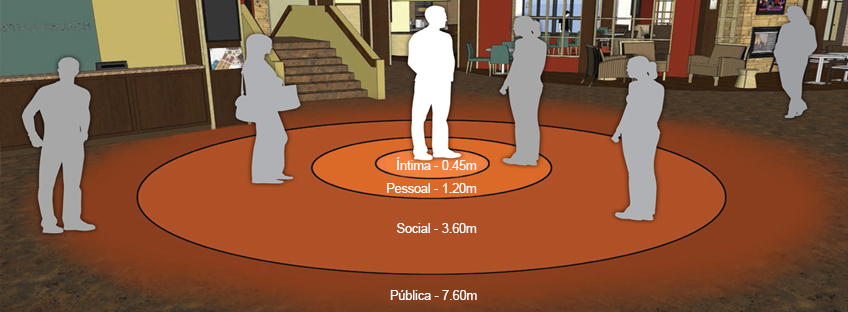
\includegraphics[width=\textwidth]{images/proxemicszones.png}
	\caption{Zonas de Proximidades definido por \citeonline{Argyle:1988}.}
	\label{fig:proximityzones}
\end{figure}

Cada uma das zonas de proximidades apresentadas na figura~\ref{fig:proximityzones} possui características particulares que pode guiar como ocorrerão as interações sociais. Na zona de proximidade social, o individuo pode emitir sons com um volume maior do que a zona de proximidade íntima que, por estarem muito próximos os indivíduos acabam se comunicando quase com sussurros. Interações na zona íntima são esperadas normalmente entre amigos muito próximos ou entre casais~\cite{Hall:1969, Argyle:1988}. O comportamento aceitável em zonas de proximidades mais distantes, como a social e a pública, é a comunicação com uma intensidade dos movimentos mais amplos e com uma força física maior que nas regiões mais próximas, onde há uma probabilidade maior de assustar o individuo com esse tipo de comportamento~\cite{Henkel:2014}.

Além dos comportamentos diferentes em cada zona de proximidade, existe um outro fator que pode atrapalhar a interação exclusiva entre duas pessoas nas regiões mais distantes. A existência de muitas pessoas ao redor das regiões mais distantes pode dificultar o estabelecimento uma interação exclusiva devido ao excesso de ruído no cenário. O ruído para esse cenário pode ser considerado através do volume excessivo de pessoas no local, junto com a altura dos sons emitidos e além da quantidade de gestos que cada individuo realiza simultaneamente~\cite{Walters:2009, Henkel:2014}.

Entretanto, não é apenas o espaço social que as \emph{Proxemics} se referem na análise comportamental. Algumas variáveis que são utilizadas para a leitura corporal também são utilizadas para a análise comportamental através das \emph{Proxemics}. \citeonline{Mead:2013} lista algumas variáveis consideradas em seu trabalho, além da distância social, são elas: (I) orientação da postura; (II) orientação do quadril; (III) orientação dos ombros; (IV) posicionamento e orientação da cabeça; e (V) fixação do olhar entre os indivíduos. Todas as variáveis apresentadas por~\citeonline{Mead:2013} auxiliam a determinar a qualidade da interação social entre dois indivíduos, agentes ou entre robôs e humanos.

\emph{Proxemics} tem sido explorado em trabalhos de interação humano-robô~(IHR) desde 1997, somando aproximadamente 25 trabalhos ao todo~\cite{Henkel:2014}. Assim, a próxima seção apresentará os trabalhos relacionados que abordam o tema da \emph{Proxemics} e as discussões sobre como eles auxiliam o trabalho apresentado nessa tese.

\section{\emph{Proxemics} e Interação Humano-Robô}
\label{sec:proxemicsihr}

Nessa seção são apresentados os trabalhos de \emph{Proxemics} aplicados a interação humano-robô~(IHR), como o trabalho de \citeonline{Walters:2009} que propõem um \emph{framework} empírico com o objetivo de auxiliar a detecção da distância real, ou seja, a distância considerando fatores diversos da IHR.

Alguns fatores de impacto na IHR foram apresentados por \citeonline{Walters:2009} na discussão de seu trabalho. Um dos fatores explorados foi o impacto dos sons emitidos pelo robô durante a interação, ou seja, a voz do robô. A voz não causa impacto apenas pelo volume que é emitida, mas também o estilo dela que pode influenciar uma vez que é possível inferir emoções a partir do estilo em que a voz é emitida. Além disso, a voz também pode influenciar no tempo de aproximação entre o robô e o individuo, pois dependendo de como o som é emitido pode gerar insegurança ao individuo que está interagindo com o robô~\cite{Walters:2009}.

Fatores como a aparência do robô e informações demográficas como idade, gênero, grau de instrução, personalidade, carisma, entre outros também podem interferir na IHR. Por exemplo, as pessoas preferem manter uma distância maior dos robôs que possuem uma aparência humanoide, pois ela causa um pouco de preocupação sobre as ações dele, quando comparado a um robô com aparência mais mecânica. Entretanto, a altura do robô não é um fator que apresenta grande relevância para IHR~\cite{Walters:2009}.

Outro trabalho, apresentado por \citeonline{Torta:2011}, tem como objetivo a apresentação de um arquitetura para robótica baseada em comportamento que permite ao robô navegar em segurança por um ambiente doméstico mutável e consiga codificar interações não verbais de maneira embarcada. Dessa maneira, é possível fazer com que o robô possa apresentar o comportamento de aproximação adequado ao seu objetivo, utilizando um novo modelo de espaço pessoal.

Esse novo modelo considera a relação entre a orientação do robô em conjunto com a distância do objetivo e ainda a avaliação do individuo para a orientação de aproximação do robô~\cite{Torta:2011}. Para alcançar esse objetivo \citeonline{Torta:2011} utilizaram um filtro Bayesiano para inferir a localização do objetivo a partir da posição do robô de maneira dinâmica. O filtro Bayesiano é utilizado como guia para o robô em seu algoritmo de navegação. 

Nos testes utilizou-se o robô NAO e obteve a validação de que a inclusão do espaço pessoal no algoritmo de navegação trouxe resultados positivos ao modelo implementado. Em estudos futuros, \citeonline{Torta:2011} incluirão outros fatores ao cenário de IHR, como a altura do robô, a aparência e o propósito da interação, e a partir dessas novas variáveis identificar como é possível melhorar a interação de tal forma, que esse modelo obtenha uma qualidade maior em sua aplicação~\cite{Torta:2011}.

A aplicação de \emph{Proxemics} não é exclusiva a robótica social ou doméstica, \citeonline{Srinivasan:2012} aplicam o conceito para o cenário de resgate de vítimas. O trabalho apresentado tem como objetivo avaliar a utilização do olhar social com movimentos de cabeça e funções escalares de \emph{Proxemics} para auxiliar na aproximação e trabalho em regaste de vítimas em centros urbanos.

Nesse cenário o robô deve manter a vítima calma, tranquila, com pensamentos positivos e cuidar dela, na medida do possível, até que o resgate consiga acesso ao local para que o trabalho de extração seja realizado com sucesso~\cite{Srinivasan:2012}. Dois cenários de simulação foram utilizados para validar o método proposto por \citeonline{Srinivasan:2012}. No primeiro cenário observou-se como a vítima correspondia a medida que o robô gesticulava com a cabeça durante a interação comparado ao robô totalmente estático. O movimento da cabeça foi programado para ficar sincronizado com a fala do robô de tal forma, que seu comportamento ficasse próximo a um comportamento natural. Neste primeiro cenário, foi validado a hipótese de que o usuário prefere o robô que tem o movimento social (gesticulação da cabeça) ao invés do robô que permanece totalmente estático durante a interação.

No segundo cenário de simulação, utilizou-se funções escalares para definir a aproximação do robô junto à vítima. Nessa aproximação são consideradas as quatro regiões de proximidades, apresentadas na figura~\ref{fig:proximityzones}, para determinar a interação com a vítima. Foram comparadas três tipos de funções: (I) Logarítmica; (II) Linear; (III) Não escalar. Nos testes os melhores resultados foram obtidos através da função logarítmica, seguida pela função linear e depois a função não escalar~\cite{Srinivasan:2012}. Dessa forma, \citeonline{Srinivasan:2012} esperam melhorar a abordagem com robôs à vítimas de desastres em cenários de centros urbanos.

\citeonline{Okita:2012} realizaram um estudo para identificar quais fatores mais auxiliam na redução da distância física entre o robô e o ser humano. Foram utilizados dois tipos de abordagem para os testes realizados: (I) Robô com a iniciativa de se aproximar do ser humano; e (II) Humano com a iniciativa de se aproximar do robô.

Para o teste de ambos cenários foram utilizados dois tipos de indivíduos, separados em dois grupos diferentes, crianças e adultos. Na execução do teste, \citeonline{Okita:2012} utilizaram o método chamado de \emph{Wizard of Oz} (WOZ) que permite operar o robô através de um controle remoto distante da vista do indivíduo em interação. Dessa forma, é possível passar a impressão de que o robô é autônomo e ao mesmo tempo ter o controle dele para que não ocorra nenhum acidente durante a interação.

O experimento foi executado de duas maneiras diferentes sendo uma o robô aproximar-se sem nenhum tipo de aviso prévio e a outra maneira era exatamente avisar sua aproximação. Observou-se que quando o robô solicitava a permissão para aproximar do individuo o resultado sempre era positivo para a interação, quando comparado à aproximação sem aviso ou com aviso posterior a ação do robô~\cite{Okita:2012}.

Muitos trabalhos apontam maneiras de aplicar o estudo de \emph{Proxemics} em interações sociais. Algumas variáveis que podem afetar a interação são funções interpessoais de relacionamento, fatores fisiológicos moldados pela cultura de origem de um indivíduo, perspectivas etnológicas, além de informações sobre o ambiente de interação, como a luz ambiente, localização e ocupação física do agente, tamanho, entre outros fatores~\cite{Mead:2011b}.

Com a facilidade de compra dos sensores de captura de movimento não invasivo como o Microsoft\textregistered\ Kinect\textregistered ou o PrimeSensor\textregistered, os pesquisadores \citeonline{Mead:2011b} apresentam em seu trabalho um conjunto de métricas que são capazes de auxiliar na automatização do processo de análise do comportamento para distância social. As métricas por eles estabelecidas são: postura, posição do quadril, do ombro, do torso, dos braços, distâncias entre os agentes, gênero, entre outros.

Com base nas métricas definidas foi realizado um estudo conceitual para verificar se o cenário com um Kinect\textregistered\ inserido no ambiente, fosse capaz de capturar todas essas informações para que a partir delas torna-se possível a criação de um mecanismo de análise automática do comportamento de agentes em um ambiente de interação social. Os testes preliminares ocorreram conforme o esperado, possibilitando a validação do cenário apresentado por \citeonline{Mead:2011b}.

Um cenário e ferramenta para coleta de informações sobre indivíduos em interação social são apresentados também por \citeonline{Mead:2011}. O principal objetivo é utilizar as informações coletadas em estudos futuros. Essas informações serviram para a criação de um modelo oculto de Markov (\emph{Hidden Markov Model} (HMM), em inglês) com seis classes para auxiliar na predição das \emph{Proxemics} de interação face a face. Nesse estudo, o HMM demonstrou-se com um desempenho superior para a tarefa de predição, quando comparado com um classificador aleatório ponderado por pesos~\cite{Mead:2011}.

\citeonline{Mead:2012} apresenta uma discussão sobre os tipos de representações para \emph{Proxemics}. Essas representações são: física e psicológica. Além desses dois tipos é proposto uma representação psicofísica que apresenta uma abordagem permitindo unir melhor as qualidades dos outros dois tipos de representação. A representação física tem como objetivo analisar como o espaço social é ocupado por dois indivíduos e é a abordagem mais comum em estudos de \emph{Proxemics}, tanto para interações humano-humano quanto para interações humano-robô. A representação psicológica mantém o foco em fatores de relacionamento interpessoal de alto nível entre dois ou mais indivíduos. Esse fatores estão relacionados a teoria de conflito afiliativo~\cite{Argyle:1965} e também a teoria de adaptação interpessoal~\cite{Burgoon:2007}. 

Porém, com as lacunas existentes nesses dois tipos de representação de \emph{Proxemics}, foi proposto o tipo psicofísico. Esse tipo de representação tem como objetivo principal analisar a percepção e a produção de estímulo social entre dois ou mais indivíduos interagindo. A abordagem psicofísica é discutida também por~\citeonline{Hall:1969}. Essa representação está diretamente ligada com a experiência sensorial do estímulo social até os parâmetros espaciais de maneira física. A partir da representação psicofísica é realizado um estudo para capturar informações que servirão de base para treinamento de dois HMM. Cada HMM é responsável por uma exclusiva tarefa, início da interação ou término da interação. Essa representação deve auxiliar nas pesquisas de interação humano-robô, no intuito de que seja possível realizar uma análise para a interação ocorrer com maior qualidade~\cite{Mead:2012}.

Outro trabalho de \citeonline{Mead:2012b} apresenta um mecanismo de análise comportamental através da \emph{Proxemics}. Utiliza-se modelos probabilísticos de tal forma, que seja possível determinar alguns comportamentos dos indivíduos durante uma interação. Como métrica de proximidade utilizou-se a estratégia do mundo de grades para predizer a distância aproximada entre o robô e o individuo. Esse trabalho é implementado através de uma rede Bayesiana dinâmica como uma melhora para o mecanismo~\cite{Mead:2012b}.

Conforme tem sido discutido ao longo dessa seção, para que a interação entre um humano e um robô possa ocorrer de maneira confortável e com qualidade, é necessário que o robô entenda as variáveis de espaço social. Além disso, é necessário também que ele possua o controle sobre essas variáveis de tal forma, que ele consiga tomar decisões sobre as ações que executará~\cite{Mead:2013b}.

\citeonline{Mead:2013b} apresentam um estudo baseado principalmente com variáveis de voz e gestos, utilizando um método de amostragem que tem como entrada a postura do indivíduo ao interagir com o robô. A maior contribuição esperada por \citeonline{Mead:2013b} é a apresentação do entendimento obtido através das interações pré culturais que estão inseridas junto ao estudo de \emph{Proxemics}. O resultado apresentado é apenas uma base de dados para investigar todos os aspectos da interação humano-robô apresentadas no trabalho (voz e gestos).

A partir da base de dados gerada por \citeonline{Mead:2013b}, é apresentado outro trabalho onde \citeonline{Mead:2013} discutem a utilização de um HMM para extração de características comportamentais espaciais do ser humano, em outras palavras, \emph{Proxemics}. Alguns fabricantes de sensores de movimentos, como o Microsoft\textregistered\ Kinect\textregistered\ e o ASUS\textregistered\ Xtion, têm pesquisado técnicas para aprimorar o estudo das distâncias sociais e também seus significados.

Com base nesses estudos, \citeonline{Mead:2013} analisam a possibilidade de automatizar o processo de análise das \emph{Proxemics}. A intenção do trabalho é extrair variáveis para que seja, então, possível determinar o início e o fim de uma interação social através de um HMM. Para realizar os experimentos foram necessários dois indivíduos e um robô aplicados a um cenário de interação, onde os indivíduos se aproximam do robô sendo que os indíviduos estão separados por uma parede. Os resultados são apresentados em relação ao ponto de vista físico e psicológico. Na detecção das variáveis que representam as \emph{Proxemics} de maneira dinâmica, \citeonline{Mead:2013} consideram os resultados satisfatórios e como sequência do trabalho é mantido o foco em interações com fatores psicológicos complexos, para aprimorar a precisão do \emph{framework} criado.

\citeonline{Mead:2014} direcionam o foco de seu trabalho para a análise de conversa social e gestos, tanto na questão de produção das conversas e gestos de maneira automática quanto para o reconhecimento, aplicados em interações humano-humano e humano-robô. Todo o trabalho realizado está relacionado com o estudo de \emph{Proxemics} na interações sociais, uma vez que essas tem o objetivo de não só identificar as variáveis, mas também de interpretar, manipular e compreender a dinâmica do comportamento espacial dentro do cenário das interações sociais.

Os estudos e experimentos sociais realizados por \citeonline{Mead:2014} auxiliaram na coleta de informações sobre o volume da fala de acordo com a distância, além dos gestos que necessitam de espaços maiores para execução sem prejudicar a interação. Os resultados apresentados apontam que a distância de interações entre humanos é menor que a distância da interação entre um humano e um robô. Além disso, os resultados obtidos não são aplicados à múltiplas culturas (nesse caso origem dos indivíduos), e isso deve ser realizado em outros trabalhos segundo \citeonline{Mead:2014}. Um mecanismo para personalizar o tratamento que o robô terá com o indivíduo durante a interação também é algo de deve ser construído ao longo dos trabalhos futuros.

Analisando a diferença de cultura para variáveis de \emph{Proxemics}, \citeonline{Eresha:2013} apresentam como objetivo do trabalho a avaliação do comportamento de indivíduos ao se encontrarem com dois robôs interagindo entre si e caminhando em direção ao individuo de tal forma que este possa também interagir ou não com os robôs conforme se aproximam. Além de avaliar o comportamento dos indivíduos durante a interação com os robôs, \citeonline{Eresha:2013} adicionaram a variável de cultura ao estudo. O objetivo é identificar como é a diferença de comportamento entre culturas diferentes. Foram escolhidos participantes de origem árabe e alemã para o estudo.

Nos experimentos, \citeonline{Eresha:2013} utilizaram dois robôs NAO que se posicionavam a 40 cm de distância entre eles e caminhavam até ficarem a uma distância diagonal de 85 cm do indivíduo. Para o experimento houve a participação de 24 indivíduos, 12 árabes e 12 alemães, sendo metade do gênero feminino e a outra metade do gênero masculino. Os testes apresentaram resultados interessantes, pois alguns indivíduos não reagiram como o esperado para pessoas de sua origem e muitas vezes o comportamento social na interação era idêntico entre alemães e árabes. Outro ponto apresentado por \citeonline{Eresha:2013} é que durante os testes dois alemães apresentaram o sentimento de medo de serem atacados fisicamente pelos robôs.

O trabalho de \citeonline{Eresha:2013} apresenta indícios de que as variáveis de \emph{Proxemics} não estão ligadas a cultura do indivíduo, como origem, mas sim na experiência cultural que este teve ao longo de sua vida. Dessa maneira, pode-se dizer que \emph{Proxemics} são variáveis extraculturais, porém é necessário realizar um tratamento para esse tipo de condição de tal forma, que o robô possa interagir com mais qualidade com pessoas que possuem diferentes experiências culturais.

\citeonline{Henkel:2012} investigam características entre diversas plataformas de teste para interação humano-robô, e com base no resultado deste estudo é realizado a proposta de uma nova plataforma de testes. A nova plataforma foi desenvolvida, pois \citeonline{Henkel:2012} alegam que não existe nenhuma plataforma de teste capaz de atender aos seis atributos de dependência das \emph{Proxemics}. Os atributos são: (I) movimento afetivo; (II) leitura das \emph{Proxemics}; (III) interação de voz; (IV) manipulação do estilo de áudio; (V) controle do olhar; e (VI) apresentação de conteúdo através de mídia, por exemplo, monitor ou leds.

A plataforma é constituída por uma cabeça feita com um monitor de 7'', junto com um encaixe construído para ser acoplado em qualquer base de robôs já existentes no mercado. Alguns testes que foram realizados no cenário de resgate à vítimas demonstram que as pessoas que tinham a zona de espaço social íntimo invadida por qualquer parte do robô sem uma interação prévia ficavam em situação de \emph{stress} elevado. Essa reação foi totalmente oposta quando o robô iniciava com qualquer tipo de interação antes de realizar a aproximação do indivíduo~\cite{Henkel:2012}. O primeiro contato antes da aproximação para uma interação maior é importante, pois esse comportamento pode definir o quão confortável a interação entre os agentes será e esse comportamento deve ser explorado durante a execução dessa tese. 

Em outro trabalho, \citeonline{Henkel:2014} apresentam duas funções escalares para avaliar os valores de proximidade entre humanos e robôs. As funções escalares são comparadas com outras funções não-escalares e também entre si de tal forma, que seja possível uma tomada de decisão em tempo de execução da ação/interação. As duas funções escalares apresentadas são: (I) logarítmica; e (II) linear.

Os testes foram executados no cenário de regaste à vitimas. Quando a função logarítmica foi aplicada, os resultados apresentados foram melhores do que os obtidos com as demais funções. Como o principal objetivo de \citeonline{Henkel:2014} é generalizar o método para outros cenários, eles pretendem realizar testes do modelo em outras situações e também utilizando outros tipos de robôs para sustentar melhor a hipótese. Os estudos prévios realizados demonstram que a generalização do modelo é possível.

A integração social do robô com os ambientes que envolvem cenários de cuidados médicos, construção, educação, serviço públicos, entre outros pode ser a chave de sua aceitação por parte dos seres humanos. Um dos caminhos para conseguir esse objetivo é fazer com que o robô saiba ter um comportamento adequado de interação em cada um desses cenários, assim como o que já é demonstrado em filmes de ficção científica. Dessa maneira, é possível fazer com que os seres humanos utilizem o próprio senso social para identificar essas habilidades no robô, quebrando um pouco o medo de interagir com ele~\cite{Heenan:2014}.

Como primeiro passo para que a interação ocorra naturalmente entre o ser humano e o robô, \citeonline{Heenan:2014} acreditam que deve haver sempre uma saudação entre ambas partes logo ao primeiro contato. Esse tipo de comportamento pode ser fundamental para que haja uma aceitação social do robô entre as pessoas. Durante uma saudação existem diversos fatores que são analisados implicitamente pelo ser humano, como nuanças de comunicação não verbal, vocalização das palavras e a distância inter pessoal. Esses fatores devem ser considerados ao projetar uma saudação por parte do robô, fazendo com que seja possível o robô iniciar a interação.

Fazer com que um robô realize uma saudação natural não é uma tarefa muito fácil. Deve ser considerado que um robô não tem a mesma capacidade de identificar as nuanças sociais com a mesma velocidade de um ser humano. Outro ponto negativo é que o robô possui o lado mecânico limitado, quando comparado a musculatura do ser humano. Assim, o primeiro objetivo do trabalho de \citeonline{Heenan:2014} é definir um subconjunto exato de elementos de uma saudação social que possa ser articulado pelo robô durante a tarefa e ainda como implementar as sutilezas do comportamento da interação de saudação social.

Os testes executados demonstram que a saudação é um ponto importante para o resultado com sucesso da interação com o ser humano. O robô NAO utilizado nos testes foi capaz de implementar ações de comportamento como o contato visual, linguagem corporal e distância social para comunicação efetiva. Apesar de algumas restrições do modelo de saudação ocorrerem devido a limitação do NAO, é possível realizar a generalização do mesmo para outros robôs~\cite{Heenan:2014}.

Percebeu-se que o contato visual se apresentou como um elemento de interação social bem natural, contudo deve-se tomar cuidado para que o robô não fique encarando a pessoa constantemente, pois é gerado um desconforto para a pessoa durante o contato. \citeonline{Heenan:2014} dizem que é possível afirmar que utilizar a saudação é importante no primeiro contato de dois agentes, além de aumentar a capacidade da interação social entre o robô e o ser humano.

\citeonline{Vazquez:2014} apresentam um robô móvel no formato de mobília, chamado Chester, construído para realizar interações com crianças. Como o Chester é muito grande optou-se por usar um segundo robô não móvel, ao qual \citeonline{Vazquez:2014} denominam \emph{sidekick}. O \emph{sidekick} é como um parceiro ou personagem secundário que auxilia as pessoas em volta a prestarem atenção no personagem principal, como por exemplo o burro da animação Shrek. O \emph{sidekick} criado é um abajur chamado Blink. Ele fica acoplado em cima do Chester. A figura~\ref{fig:vazquez} apresenta a combinação dos robôs Chester e Blink.

\begin{figure}[ht!]
	\centering
	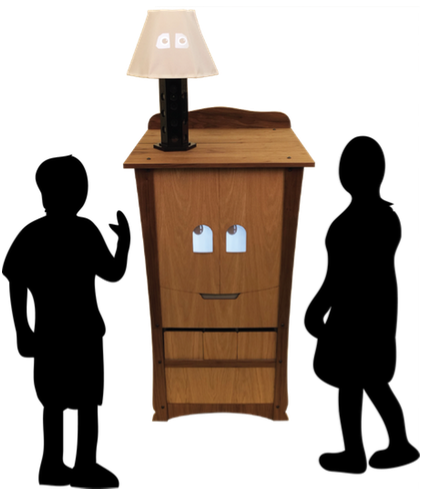
\includegraphics[width=0.4\textwidth]{images/vazquez2014.png}
	\caption{Chester e Blink os robôs apresentados por \citeonline{Vazquez:2014}.}
	\label{fig:vazquez}
\end{figure}

Blink tem uma linguagem própria e apenas o Chester é capaz de entender. É como o R2D2 em Star Wars que apenas alguns personagens são capazes de compreende-lo e falar com ele diretamente. Os resultados obtidos mostram que a inserção de um \emph{sidekick} não altera a questão de proximidade das crianças em relação ao robô, mas melhora a atenção com os elementos falantes do cenário~\cite{Vazquez:2014}.

Foi possível caracterizar alguns comportamentos das crianças ao interagir com os robôs. É afirmado por \citeonline{Vazquez:2014} que o formato de mobília para robôs é plausível para utilizar em robôs que interagem com crianças, pois elas se sentem mais empáticas aos robôs. Contudo, é questionável essa afirmação. Será que o que realmente influenciou esse resultado foi o formato do robô ou foi seu comportamento durante o contato com as crianças? Provavelmente, esse é um resultado que pode ser obtido com a mistura desses dois fatores, aparência e comportamento.

Por questões de segurança os testes foram executados utilizando o método \emph{Wizard of Oz} (WoZ), onde existe um especialista controlando o robô através de um controle de videogame, por exemplo. Foram conduzidos duas variantes do teste, são elas: (I) com o \emph{sidekick} ativo; e (II) com o \emph{sidekick} inativo. O especialista que controla o robô encontrava-se na mesma sala de teste, mas algumas precauções foram consideradas para que não houvesse ruído nos resultados do teste. Uma dessas precauções foi inseri-lo na sala do teste antes do mesmo iniciar para que aparenta-se que ele estava apenas trabalhando normalmente. Além disso, o controle do robô foi posicionado embaixo da mesa para facilitar a oclusão do objeto e ainda fez com que nenhuma criança notasse que o robô era teleoperado por um especialista~\cite{Vazquez:2014}.

Para capturar as informações de distância foi acoplado ao teto um sensor Microsoft Kinect. Ele é responsável por capturar as informações de distância entre o robô e a criança interagindo com ele. Notou-se que na maioria das vezes a criança ficava sempre de frente a face do robô e não ao seu lado ou atrás dele. Variáveis como o tempo de resposta para se afastar enquanto o robô dizia ``recue'' também foi considerado para identificar os resultados~\cite{Vazquez:2014}.

Nos resultados finais, \citeonline{Vazquez:2014} encontraram algumas limitações do robô e também do experimento, como por exemplo, o pouco conteúdo de linguagem que o robô possui implementado para dar respostas aos participantes do teste. Outro problema encontrado foi no início e no final de interação onde outros pontos do cenário e tarefa atrapalharam a coleta de informações ou melhor o foco do caso de estudo. Devido a esse problema, a utilização de um \emph{sidekick} deverá ser estuda com mais detalhes e realizar os testes novamente para que possa ser comprovado o real benefício dele nos resultados da interação. Resultados preliminares confirmam que o \emph{sidekick} não atrapalha na interação entre o robô principal e as pessoas e ainda auxilia a aumentar a atenção das pessoas o que auxilia em um melhor comportamento reativo dos participantes~\cite{Vazquez:2014}.

Alguns estudos utilizando robôs para interagir com crianças com autismo apontam que pode apresentar reações positivas e negativas para o âmbito social. Especialistas são capazes de identificar esse tipo de avaliação através da análise dos vídeos gravados entre sessões. O objetivo do trabalho de \citeonline{Feil-Seifer:2010} é automatizar esse processo de análise através do uso de robôs. Para isso foi desenvolvido um classificador heurístico para discretizar as crianças que conseguem interagir com o robô daquelas que não conseguem.

O cenário de teste é composto de uma sala, um robô totalmente autônomo com o objetivo de incentivar a interação, uma criança diagnosticada com autismo e um familiar mais próximo. Para incentivar a interação o robô deve se aproximar apresentando vocalizações de sons felizes e também esboçar um sorriso para a criança, por exemplo. Caso alguma criança se afaste do robô, ele deve esboçar uma face triste e emitir sons que demonstre a sua não felicidade~\cite{Feil-Seifer:2010}.

Durante os testes foram gravados vídeos e algumas marcações foram realizadas no robô, e nos pais, com o intuito de auxiliar na medida das distâncias entre a criança e o robô ou seus pais. Para realizar uma avaliação sobre esse cenário foi utilizada a seguinte heurística: Para cada trecho de tempo se a criança encontrar-se a 0,85 m dos pais ela é considerada próxima à eles. Caso ela encontra-se a 0,5 m de uma parede ela é considerada próxima a parede. Para ser considerada atrás do robô ela deveria estar a qualquer distância, mas entre uma angulação maior que 135º e menor que -135º~\cite{Feil-Seifer:2010}.

A partir das informações capturadas é possível gerar o classificador onde ele análise se pelo menos 50\% do tempo gasto é com as informações de comportamento negativo (mapeado pelas heurísticas), então é considerado que a criança não deseja interagir com o robô. Caso contrário, menos de 50\% do tempo gasto, a criança deseja interagir com o robô. Apesar dos resultados positivos, esse classificador não deve ser considerado como regra para que haja uma maior escalabilidade do projeto e sua aplicação~\cite{Feil-Seifer:2010}. Esses tipos de parâmetros podem auxiliar na determinação de interação ou não interação. Dessa forma, pode-se fazer com que o robô recue ou tente uma nova abordagem, para quando a reação do indivíduo for negativa.

Outros estudos confirmam a existência de uma relação de distância social entre o robô e o ser humano, entretanto nenhum método foi proposto computacionalmente para que haja uma geração do comportamento em relação a essa distância~\cite{Henkel:2012b}. Assim, é apresentado um método escalar do comportamento do robô de tal forma, que esse comportamento baseado na distância social tenha como suporte uma lei física e duas psicológicas: \emph{inverse-square law}, \emph{Weber-Fechner law} e \emph{Steven's Power law}~\cite{Henkel:2012b}.

O cenário de teste é um ambiente de desastre no qual o robô deve localizar a vítima. A interação ocorre por meio de voz sintetizada, caminhos pre definidos e controle segundo o módulo de teste WoZ. Como meio de avaliação questionários pré e pós interação são aplicados aos usuários que participam do teste~\cite{Henkel:2012b}.

Atributos primários foram determinados para que possam ser identificados alguns níveis de consistências sociais: conforto, movimentos naturais, consideração do espaço pessoal, segurança e controle próprio. Atributos secundários também foram considerados nos estudos de \citeonline{Henkel:2012b}, são eles: atenciosidade, empatia, felicidade, similaridade, inteligência, sensibilidade, submissão e confiança. Os resultados demonstram que todos atributos primários e apenas três secundários provaram que apresentam melhor significância para o processo. O sistema de percepção escalar provou ser melhor do que o não escalar. O modelo escalar linear apresentou o mesmo resultado que o não escalar~\cite{Henkel:2012b}.

\citeonline{Hemmert:2013} apresentam um trabalho que tem como objetivo a aplicação dessa técnica em aparelhos de telefonia móvel. A ideia principal é fazer com que o telefone reaja de acordo com a aproximação do aparelho pela voz da pessoa. O foco principal dentre as oito variáveis de \emph{Proxemics} é a postura do usuário. Interações de \emph{Proxemics} tem sido um dos modelos gerais em interação humano-computador (IHC). Entretanto, é um tema pouco explorado em telefonia móvel~\cite{Hemmert:2013}.

O projeto utilizado no caso de estudo apresenta uma nova maneira de interagir com dispositivos móveis, em especial telefones, tendo como base variáveis de linguagem corporal e proximidade do indivíduo para com o aparelho. Como trabalho futuro \citeonline{Hemmert:2013} querem apresentar um modelo que faça a leitura de diversas variáveis com o intuito de entender por completo como elas funcionam no comportamento do ser humano.

Um ponto interessante abordado por \citeonline{Hemmert:2013} é quando ele faz refêrencia ao uso de \emph{Proxemics} em IHR. Geralmente os trabalhos de \emph{Proxemics} são voltados ao comportamento de ser humano, e nenhum possui foco na reação do robô, ou seja, como esse robô reagirá caso um ser humano invada o espaço íntimo do robô sem consentimento. Esse é um ponto interessante que deve ser explorado ao longo dessa tese. 

Outro ponto chave dos trabalhos apresentados ao longo dessa seção é que sempre utilizam sensores no ambiente para medir as variáveis de \emph{Proxemics} entre a pessoa e o robô. Contudo, acredita-se que esse tipo de abordagem não é natural ao robô móvel, pois os seres humanos não tem o auxílio sendo assim o robô também não deve utilizar desses recursos. Contudo, as variáveis de \emph{Proxemics} se mostram essenciais para determinar o sucesso de uma interação ou não, e devem ser consideradas ao longo da proposta desta tese de doutorado.

Dessa forma, todas as variáveis apresentadas nos trabalhos dessa seção são importantes para avaliar o comportamneto de um indivíduo durante uma interação com robôs e até outros dispositivos tecnológicos. Na seção~\ref{sec:extracaocaracteristicas} são apresentados as variáveis consideradas para o desenvolvimento desse trabalho. Além das variáveis, também são avaliados os meios de captura das informações visando a aplicação do trabalho desenvolvido na tese inserido em um ambiente inteligente.
% %!TEX root=Principal.tex
\chapter{INTERAÇÃO HUMANO-ROBÔ}
\label{cap:ihr}
Interação Humano-Robô (IHR) é a área de estudo que procura compreender, avaliar e implementar robôs para que possam trabalhar em conjunto ou executar uma determinada tarefa onde a interação com o ser humano ocorra. A interação deve ser menos invasiva e mais colaborativa. O primeiro guia da IHR apareceu no conjunto de trabalhos de ficção científica de Isaac Asimov, que é apresentado como as primeiras leis da robótica por diversos prioneiros no tema. A primeira lei fala que um robô não pode ferir um ser humano e também deve proteje-lo para que nenhum mal o seja causado. A segunda lei diz que um robô deve obedecer as ordens dadas por seres humanos exceto nos casos que as ordens entrem em conflito com a primeira lei. E por fim a terceira lei diz um robô deve proteger sua própria existência desde que não entre em conflito com a primeira e/ou segunda leis. Essas leis regem os trabalhos em IHR até os dias atuais~\cite{goodrich:2007, weiss:2010}.

Qualquer tipo de robô possui um nível de interação, mesmo os completamente autônomos. A interação pode ocorrer de duas maneiras específicas: Interações Remotas (robôs e humanos em diferentes locais espaço-temporais), por exemplo, a operação do robô Curiosity\footnote{https://www.nasa.gov/mission\_pages/msl/index.html} em Marte e a NASA no planeta Terra; Interações Próximas (robôs e humanos estão no mesmo local, compartilhando o mesmo espaço), por exemplo, em indústrias ou residências como o robô Roomba~\cite{goodrich:2007}.

Robôs teleoperados são guiados por controles, como por exemplo \emph{joysticks} de video games. Já os robôs completamente autônomos devem consistir o ambiente, o cenário de atuação, agentes existentes no ambiente e os que estão direcionando-o para o seu objetivo final, além de atualizar constantemente esses dados e as restrições competentes. Muitos trabalhos são direcionados a interação através de um controle ou central de comando com a operação de um ser humano, mas a quantidade de trabalhos com robôs autônomos vêem crescendo principalmente em pesquisas de robótica assistiva e robótica para resgate em catástrofes, onde existem riscos a vida~\cite{goodrich:2007, weiss:2010}.

IHR é um estudo que necessita da participação de diversas outras áreas de pesquisa, como Ciências Cognitivas, Linguística, Psicologia, Antropologia, Engenharia, Ciências da Computação, Matemática, Engenharia dos Fatores Humanos e Design. É importante também, o estudo de padrões de interação adotadando pequenas perspectivas sobre soluções de problemas condizentes com a pesquisa, tornando mais fácil encontrar meios de corrigir um problema recorrente~\cite{goodrich:2007}.

Uma definição para interação é a atividade de trabalhar em conjunto para o mesmo objetivo. A IHR é afetada por cinco fatores de interação, que são: (I) Nível e comportamento de autonomia; (II) Troca natural de informação; (III) Estrutura do time; (IV) Adaptação, aprendizado e treinamento de pessoas e robôs; e (V) Definir as tarefas. Um robô que possui um grau de autonomia, consegue manter-se desatento por um período de continuar sua tarefa no mesmo ponto que parou. Contudo, em IHR a autonomia não é considerada com um resultado final, mas sim um meio que auxilia o processo de interação~\cite{goodrich:2007, weiss:2010}.

O nível de autonomia de um robô determina o quanto esse pode agir por conta própria. Existem diversas formas de medir e analisar esse nível. O mais utilizado é a escala de Sheridan~\cite{sheridan:1978} que apresenta um intervalo continuo desde de um robô que não realiza nenhuma tarefa por conta própria, ou seja, um robô teleoperado, até um robô totalmente independente e autônomo. Apesar do grande uso da escala de Sheridan, sua aplicabilidade ao cenário completo não é muito eficiente. Aconselha-se utilizar a escala dividindo o cenário em subtarefas~\cite{goodrich:2007, weiss:2010}.

Em IHR o nível de autonomia é melhor determinado por uma combinação entre o nível de interação com o humano e o quanto ambos, robô e pessoa, conseguem realizar tarefas de forma independente. O desenvolvimento de habilidades cognitivas é importante para o robô interagir com o humano de maneira natural e eficiente. Nos anos 80, Brooks apresentou um novo paradigma para autonomia de robôs, conhecida como robôs baseados em comportamento~\cite{brooks:1986, brooks:1991}. Outro modelo chamado de sinta-pense-aja também é apresentado na literatura como uma arquitetura híbrida que apresenta um problema de desenvolver comportamentos naturais e atividades robustas para robôs humanoides. Devido a isso, as áreas que trabalham no modelo cognitivo de aprendizagem e tomada de decisão tem crescido cada vez mais~\cite{goodrich:2007}.

Estudos de interação entre humanos e robôs não se limitam apenas ao nível de autonomia do robô. Modelos cognitivos, aplicações em ambientes sociais e principalmente em ambientes de cuidados pessoais, têm se tornado cada vez mais frequentes em novos estudos.

% Computação Afetiva
O tratamento de inteligência emocional em trabalho de IHR tendem a tornar as tarefas realizadas mais naturais. \citeonline{rani:2006} apresentam um modelo dos efeitos fisiológicos e correlaciona com os psicofisiológicos para que o robô seja capaz de inferir sobre o efeito da ansiedade nas pessoas. A partir desse modelo foi possível incentivar a melhora no desempenho de pessoas que tentavam fazer cestas em um jogo de basquete.

% IHC
Outro ponto fundamental é a utilização de técnicas sólidas em Interação Humano Computador (IHC) como base para solucionar problemas em IHR. A técnica de GOMS (\emph{Goals, Operators, Methods and Selections}) foi adaptada para entender projetos de IHR como modelos de processamento humano. Assim, a modelagem de tarefas do robô em diversos cenários pode ter benefícios e maior efeciência na execução~\cite{drury:2007}.

% Aprendizado por demonstração
\citeonline{giovannangeli:2007} apresentam um modelo de IHR onde o robô é capaz de aprender tarefas a partir de uma pessoa realizando o papel de treinador, onde o robô reproduz seus movimentos e consegue armazená-lo para situações futuras. No mesmo sentido, um trabalho com o robô Pepper da Softbank é apresentado por \citeonline{kitagawa:2016}. Nesse trabalho é realizado um controle de \emph{sleep} antes da reprodução dos gestos. Esse controle auxiliou na naturalidade da execução dos gestos e também um fato curioso, foi que a pessoa reproduzindo os gestos muitas vezes acabava por imitar o robô.

% Aparência
Outro fator importante para IHR é a aparência do robô em conjunto com a capacidade de execução de tarefas esperada para àquela aparência. Dessa maneira, \citeonline{minato:2007} apresentam uma plataforma robótica em formato de uma criança, mais precisamente um bebê, para realizar estudos de interação e principalmente a capacidade da cognição do robô durante a interação.

% Teorias de Psicologia (mente, ação)
Diversas teorias de psicologia também são aplicadas em trabalhos de IHR. Um exemplo é a teoria da mente que auxilia o robô na análise do comportamento de um indivíduo e possibilita a tomada de decisão para uma interação próxima a natural~\cite{hiatt:2011}. Assim como a teoria de ação, definida por Norman, que auxilia na definição de emoções humanas com base em ações tornando o comportamento do robô mais natural ao do ser humano~\cite{toumi:2013}.

% Plataformas de Teste
Utilizando um sensor de movimento Kinect foi criado uma plataforma de teste para interação humano-robô, onde o ser humano pode treinar o robô a distância e sem necessidade de contato físico. A idéia é poder fazer com que o robô não cause dano físico à pessoa e por consequência diminuir o medo de interação em participação de testes. A plataforma apresentada por \citeonline{rossmann:2013} transmite em tempo real o conhecimento dos gestos para o robô e este é reproduzido fielmente.

% Assistência Médica
Aplicações em serviços médicos também são explorados em IHR. \citeonline{briggs:2015} apresentam um estudo para auxiliar o tratamento de pessoas com a doença de Parkinson. Com essa doença o paciente pode perder a funcionalidade dos muscúlos faciais, levando assim a perda das expressões faciais. Quando um enfermeiro ou médico vai realizar o tratamento do paciente, pode interpretar que ele está desdenhando ou com nojo do profissional. A utilização do robô soluciona esse problema, já que o robô é capaz de filtrar as expressões faciais. Nos testes apresentados, os pacientes sentiram-se confortáveis com a interação junto ao robô NAO da Aldebaran.

% Colaboração
Trabalhos colaborativos são amplamente explorados entre os trabalhos de IHR. Muitos trabalhos vem promovendo debates sobre o assunto~\cite{strohkorb:2016,lampe:2016}. Alguns trabalhos já apresentam a integração com outros tipos de técnicas para desmontrar como que o robô pode assumir a liderança na tarefa ou apenas seguir as instruções da pessoa. Um trabalho nessa direção é apresentado por \citeonline{li:2015} que utiliza a teoria de jogos para solucionar o problema de lider ou seguidor na IHR.

% Casa Inteligente
Sistemas de detecção de anomalias com o propósito de servir idosos e pessoas com problemas físicos que vivem sozinhos é outro tema explorado. Após a detecção da anomalia com base no padrão de interação com o ambiente dessa pessoa, as entidades de assistência domésticas são acionadas e o processo de socorro da pessoa é iniciado. Para que esse trabalho atingisse uma boa acurácia (entre 80\% e 85\%), um robô móvel é utilizado em conjunto com senhores no ambiente de uma casa inteligente para detecção das anomalias~\cite{lundstrom:2015}.

% Educação
Como pode-se observar, a IHR tem sido aplicada em diversas áreas de atuação e uma que cresceu o número de trabalhos dedicados é a área da educação. \citeonline{martelaro:2016} investigam métodos para criação de comportamento do robô em função de aumentar a confiança entre humanos que interagem com robôs. Dois meios de medida para o aumento da confiança são aplicados, vulnerabilidade vs expressividade. Notou-se nos testes que robôs mais vulneráveis aumentam mais a confiança do que robôs mais expressivos. Os testes foram realizados com base em um robô tutor.

Outra proposta é identificar se crianças conseguem aprender melhor com o um tutor humano ou um robô. Estatisticamente, não houve significância considerável entre os dois resultados. Porém, o índice de Carson mostrou que o humano conseguiu ser melhor que o robô, principalmente na questão social. Um dos pontos que mais faltaram ao robô durante a interação com as crianças foi a questão de olhar mútuo. Apesar do estudo feito, não existe a ideia de substituir o ser humano com o robô, mas sim utilizar o robô como uma ferramenta complementar na sala de aula~\cite{kennedy:2016}.

% Robótica de Serviço
Um questionário é conduzido dentro de um hotel no Japão que utiliza de robôs para realizar alguns serviços. O objetivo é identificar se o robô é capaz de substituir uma pessoa nas tarefas. Entrevistaram em primeiro lugar o gerente do hotel e depois direcionaram as entrevistas às pessoas que tinham maior contato com o robô no dia-a-dia. Chegou-se a conclusão de que robôs podem substituir o ser humano nas tarefas, porém esse é um trabalho que deve ser realizado de maneira bem planejada~\cite{osawa:2017}.

Um robô com aspecto de humanoide foi desenvolvido para fazer a patrulha de um shopping durante a noite e durante o dia servir de apoio ao visitantes. A área de segurança deve ser muito explorada, pois a quantidade de pessoas treinadas para executar esse trabalho tem diminuído e as empresas não estão conseguindo repor a necessidade do mercado. Como patrulha, o robô teve um desempenho esperado, só que a atuação como cartão de boas vindas ao shopping foi além do esperado. Os resultados mostraram que as pessoas tiveram empatia pelo robô e acabou fazendo com que ele atraísse mais consumidores ao shopping~\cite{lopez:2017}. Isso demonstra que o robô pode apresentar múltiplas aplicações, apenas trocando as funções de seu programa.

% Aprendizado
Para que o robô seja capaz de realizar todas essas atividades, várias técnicas devem ser empregadas. Para realizar a personalização da interação do robô para cada pessoa, \citeonline{suga:2006} aplicam uma técnica de computação evolucionária interativa. Essa técnica funciona como um algoritmo evolucionário qualquer, porém a função \emph{fitness} é dada pela avaliação direta da pessoa. Como meio de melhorar essa função, é apresentado uma função híbrida onde uma parte dos genes são modificadas pelo usuário e outra parte modificada pelo próprio algoritmo usando como base as modificações manuais. Os resultados apontaram que o robô foi capaz de adaptar o comportamento de cada sujeito de teste.

Outro algoritmo evolucionário é aplicado para melhorar a aparência do robô com a ajuda e retorno sobre o gosto da pessoa. A fase de seleção do algoritmo era feita sobre a preferência do usuário que avaliava uma versão digital da morfologia do robô. Após o estacionamento da aparência do robô na otimização feita pelo algoritmo, o robô era confeccionado~\cite{debeir:2016}.

% Eyetracking
O uso da percepção sobre o olhar em uma interação entre humanos é comum e auxilia a melhorar a comunicação entre os indivíduos. A abordagem dessa característica é pouco utilizada em interação humano robô e geralmente é realizado com base na orientação da cabeça apenas. Utilizar a orientação da cabeça pode gerar um erro grande e uma noção de comunicação falha. Por isso, \citeonline{palinko:2016} desenvolveram um algoritmo de rastreamento do olho com baixo custo passivo para um robô humanoide. Os resultados apresentaram um bom rastreamento do movimento do olho. Agora estudos tendem a evoluir para o rastreamento da pupila e da posição da cabeça para melhorar a robustez do algoritmo.

% Contato físico
Tratando-se de IHR é impossível não tratar a questão do contato físico entre os agentes. Com base nessa premissa, foi criado um modelo de controle de impedância, para reduzir e controlar a força do robô após o contato com qualquer superfície. É utilizado um sensor de RGB-D (Kinect) para identificar o ponto de contato e em seguida o planejamento do movimento é feito. Caso haja um contato não planejado durante sua trajetória, o robô é capaz de identificar a pressão exercida, regulando assim a força exercida sobre a superfície mantendo a segurança na interação~\cite{magrini:2015}.

Outra questão investigada na interação com contato físico é o efeito de um abraço dado por um robô de pelúcia gigante sobre a vontade de fazer caridade das pessoas abraçadas. Resultados não foram estatisticamente significantes, porém acreditasse que é necessário realizar uma investigação melhor sobre essa questão~\cite{nakata:2017}.

% Falha de Sistema
É investigado também a questão sobre a preocupação com a segurança pessoal ou o custo financeiro dos danos causados pelo robô em caso de falha. Para conduzir o experimento alguns videos de situações e tarefas de interação humano-robô foram apresentados para pessoas. Após o video elas avaliavam o grau de criticidade de cada situação.
Os resultados apresentados são interessantes, pois as pessoas deram um nível maior de criticidade para o robô derrubando líquido no laptop do que ele esbarrar e machucar uma pessoa. Contudo, estudos mais realísticos devem ser efetuados~\cite{adubor:2017}.

% UX
O aumento de trabalhos com IHR vêem tomando uma proporção grande. Dessa maneira, pesquisadores em experiência de usuário tem se mobilizado para entender com as pessoas estão se sentindo em relação a essa nova tecnologia e como melhorar a experiência com ela. \citeonline{lindblom:2016} defendem essa ideia e falam que é o melhor caminho para o desenvolvimento de robôs sociais com maior aceitação. Utilizar tais técnicas torna-se importante, pois auxiliam em aspectos que aumentam a aceitação, usabilidade e credibilidade dos sistemas robóticos em âmbito social. Para auxiliar os futuros projetos de robótica, os autores informam sobre 3 desafios que devem ser vencidos ao longo dos próximos anos:

\begin{itemize}
    \item Adoção de um processo iterativo de UX design;
    \item Incorporar metas de UX para garantir uma boa experiência;
    \item Projetistas de robótica devem adquirir o conhecimento adequado para a avaliação de UX.
\end{itemize}

É importante olhar cada um desses desafios, pois a aplicação de UX em HRI fará com que os robôs sociais sejam melhor aceitos em diversos ambientes e por pessoas dos mais diferentes perfis~\cite{lindblom:2016}.

% Privacidade, Segurança e Ética
Outras discussões também tem sido endereçadas na questão de robótica social, assistiva e de serviço. Com robôs entrando em nosso dia-a-dia começa a preocupação sobre questões de invasão de privacidade das pessoas por parte destes agentes. Questões éticas sobre a aplicação dos robôs no dia-a-dia. Essas linhas de pesquisa têm ganhado força em debates da comunidade~\cite{rueben:2017}.

Ao observar os trabalhos relacionados a IHR, pode-se perceber que quando existe uma interação social, o primeiro passo é a aproximação entre dois agentes. Dessa forma, existe a necessidade do robô aprender como se comportar, de acordo com algumas normas sociais, durante a aproximação de um ser humano. Assim, um modelo é apresentado com o objetivo principal voltado para o mapeamento do espaço social e também a análise do comportamento humano. Este modelo tem como sua essência um conceito apresentado por \citeonline{hall:1969}, chamado de \emph{Proxemics}. O modelo serve de base para essa tese e é apresentada em detalhes no capítulo~\ref{cap:proxemics}.

% %!TEX root=Principal.tex
\chapter{RACIOCÍNIO BASEADO EM CASOS}
\label{cap:rbc}

Raciocínio Baseado em Casos (RBC) é uma metodologia utilizada em Inteligência Artificial que constrói e utiliza um sistema de base de conhecimento criado a partir de experiências passadas. Esse tipo de comportamento é basicamente o comportamento que os seres humanos têm ao solucionar problemas similares com diferentes experiências obtidas ao longo de suas vida~\cite{Lopez:2013}.

O RBC tenta encontrar sempre uma solução, igual ou parecida com a situação atual, em sua base de conhecimento. Ao encontrar essa solução ou possível solução, o RBC tenta adapta-la da melhor maneira à tarefa atual. Caso não seja identificado nenhum caso similar ao atual sendo a situação totalmente nova é possível inferir uma sequência de ações para o caso e armazena-la para que possa ser consultado ao longo do seu ciclo de vida~\cite{Lopez:2013}.

A metodologia do RBC apresenta quatro fases principais. Essas fases são apresentadas na figura~\ref{fig:rbcciclo}~\cite{Lopez:2013}.

\begin{figure}[h!]
	\centering
	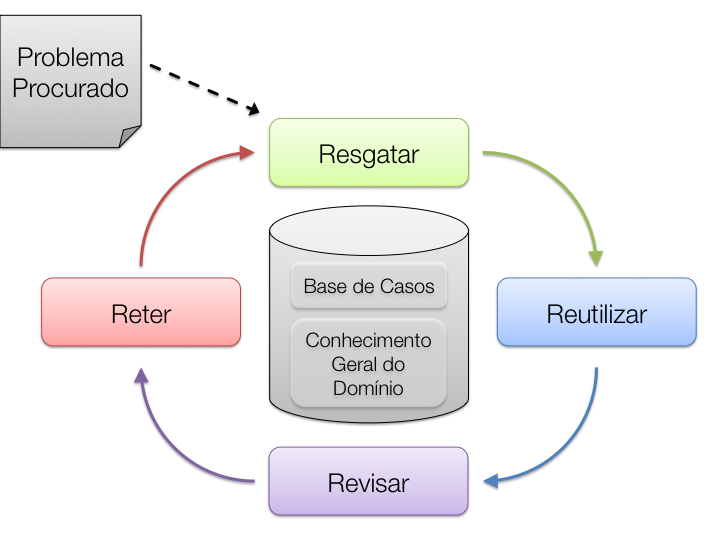
\includegraphics[scale=0.5]{images/cbr-cycle.png}
	\caption{Ciclo da Metodologia de um sistema de RBC.}
	\label{fig:rbcciclo}
\end{figure}

A seguir são apresentadas as fases da figura~\ref{fig:rbcciclo} em detalhes:

\begin{enumerate}
	\item \textbf{Resgatar}: Nessa fase são resgatados casos passados similares ao caso procurado. Métodos indutivos são aplicados normalmente para encontrar os casos armazenados em memória.
	\item \textbf{Reutilizar}: A partir de um conjunto de soluções similares resgatadas formam a base para a construção de uma solução ao problema procurado. A transformação que pode ser obtida nessa fase, ocorre através de generalização e especialização dos casos resgatados.
	\item \textbf{Revisar}: Verificar se a solução apresentada para o problema procurado provem ou não a saída desejada.
	\item \textbf{Reter}: Quando a solução apresenta ao problema gera uma nova experiência, esta pode ser ou não armazenada na base de casos. Para que o armazenamento seja realizado, é confrontado o valor obtido como resposta no processo de revisão do caso, junto com a política de retenção implementada no sistema.
\end{enumerate}

O modelo apresentado na figura~\ref{fig:rbcciclo} é baseado no nível de conhecimento que sistema pode representar. Ele identifica todo o ciclo da metodologia de RBC, do começo ao fim. Esse modelo também é conhecido como 4R’s, pois os nomes dados para cada uma das fases são iniciados com a letra R~\cite{Lopez:2013}.

%%%%%%%%%%%%%%%%%%%%%%%%%%%%%%%%%%%%%%%
\section{Classificação de sistemas de RBC}
\label{sec:classificacaorbc}

Para que sejam construídos, os sistemas de RBC consideram quatro critérios básicos que definem sua topologia~\cite{Lopez:2013}: Fonte de Conhecimento, Função, Organização e Maneira de Distribuição. A tabela~\ref{tab:classificaorbc} apresenta os possíveis tipos para cada um dos critérios.

\begin{table}[h!]
	\centering
	\caption{Classificação de Sistemas de RBC de acordo com sua topologia}
	\begin{tabular}{c | c | c | c} \hline
		Fonte de & Função & Organização & Maneira de \\ 
		Conhecimento & & & Distribuição \\ \hline
		- Textual & - Classificação & - Exclusivo & - Memória Única \\ 
		- Estrutural & - Recomendação & - Níveis Múltiplos & - Memória Múltipla \\
		- Conversacional & - Tutoria & - RBC Híbrido & - Agente Único \\
		- Temporal & - Planejamento & - Meta RBC & - Agente Múltiplo \\
		- Imagens & - Monitoramento & & \\
		& - Gerenciamento de & & \\ 
		& Conhecimento & & \\ \hline
	\end{tabular}
	\label{tab:classificaorbc}
\end{table}

O primeiro atributo apresentado na tabela~\ref{tab:classificaorbc}, Fonte de Conhecimento, refere-se em como é estrutura ou armazenamento do conhecimento passado no sistema. São eles~\cite{Lopez:2013}:

\begin{enumerate}
	\item \textbf{Textual}: É uma coleção de informações em formato de texto, que devem ser lidas pelo sistema afim de identificar a solução do problema. Um exemplo são sistemas do tipo FAQ, que podem ser encontrados em diversas ferramentas e aplicativos.
	\item \textbf{Estrutural}: É definido através de um vocabulário pré definido do problema. Cada caso pode englobar uma quantidade n de variáveis, como por exemplo, um sistema médico que possui informações como idade, histórico de atendimento, índice de massa corpórea, entre outros.
	\item \textbf{Conversacional}: Nesse tipo de RBC o caso é definido maneira iterativa através de um sistema de conversa entre usuários e/ou usuário-sistema, como por exemplo, um sistema de help-desk.
	\item \textbf{Temporal}: Quando os casos possuem uma relação temporal entre si, seja essa relação implícita ou explicita. Um exemplo desse tipo de sistema é o histórico de jogo de um usuário.
	\item \textbf{Imagens}: Cada caso é obtido através do conhecimento extraído na análise das imagens armazenadas no banco de dados. Essa análise ocorre de acordo com alguns fatores relevantes ao domínio do problema e encontrados nas imagens.
\end{enumerate}

O atributo Função refere-se ao objetivo de aplicação do RBC, ou seja, qual o tipo de problema que ele procura resolver. Abaixo a descrição detalhada de cada uma das funções que um sistema de RBC pode apresentar~\cite{Lopez:2013}:

\begin{enumerate}
	\item \textbf{Classificação}: Utilizado geralmente em aplicações onde existe a necessidade de predizer uma classe ou rótulo. Pode ocorrer de duas maneiras: (I) Através da prognosis sendo feita por duas classes, uma positiva e outra negativa; ou (II) Através do diagnóstico sendo feita por um número discreto de classes para predição.
	\item \textbf{Recomendação}: Utilizado para recomendar algum tipo de produto baseado na similaridade das escolhas passadas do usuário.
	\item \textbf{Tutoria}: Utilizado para buscar uma coleção de exercícios de uma determinada disciplina e assim auxiliar o usuário.
	\item \textbf{Planejamento}: Utilizado em duas tarefas normalmente.  A primeira é deixar o planejamento de um processo ou sistema mais eficiente e a segunda tarefa é realizar o raciocínio e aprendizado a nível de planejamento e não a nível da ação de execução como os demais RBC's.
	\item \textbf{Monitoramento}: Utilizado para predizer anomalias de comportamento durante a supervisão de sistemas, principalmente.
	\item \textbf{Gerenciamento do Conhecimento}: Utilizado para fontes de informação e avaliação do conhecimento, não só lembrando da experiência obtida, mas também aplicando esse conhecimento na solução de tarefas.
\end{enumerate}

O atributo Organização refere-se a combinação de RBC para solução de problemas em um mesmo domínio. A Organização também pode ser encontrada como arquitetura do sistema de RBC. As quatro principais são~\cite{Lopez:2013}:

\begin{enumerate}
	\item \textbf{Exclusivo}: Nessa configuração um único RBC é considerado para resolver o problema.
	\item \textbf{Níveis Múltiplos}: Nessa configuração é considerado um determinado número de RBC para solucionar o problema. Uma aplicação desse tipo de arquitetura é a interpretação de imagens.
	\item \textbf{RBC Híbrido}: Essa configuração é aplicada em problemas que necessitam de soluções híbridas ou complementares. Um exemplo de aplicação é o sistema que realiza o diagnóstico de uma doença combinado com outro sistema que realiza o planejamento para o tratamento dessa doença.
	\item \textbf{Meta RBC}: Essa configuração é utilizada quando existe vários sistemas de RBC que necessitam ser aplicados à um único domínio e é utilizado um segundo sistema RBC que verifica qual é o melhor sistema para ser aplicado dado um determinado caso.
\end{enumerate}

É importante ressaltar que o RBC é uma metodologia e não uma tecnologia. Portanto, cada fase dele pode ser resolvida por diversas técnicas de Inteligência Artificial~\cite{Lopez:2013}.

O último atributo que é apresentado na tabela~\ref{tab:classificaorbc} chama-se Maneira de Distribuição. Ele é caracterizado pela maneira como será feita o processamento dos casos. São classificados em dois critérios apenas: (I) Memória ou o número de casos existentes na base de conhecimento; e (II) Forma de distribuição do processamento, sendo possível em um único sistema ou em múltiplos sistemas. Dessa maneira, é obtido quatro possíveis combinações, são elas~\cite{Lopez:2013}:

\begin{enumerate}
	\item Memória Única, Agente Único;
	\item Memória Única, Agente Múltiplo;
	\item Memória Múltipla, Agente Único;
	\item Memória Múltipla, Agente Múltiplo.
\end{enumerate}

%%%%%%%%%%%%%%%%%%%%%%%%%%%%%%%%%%%%%%%
\section{A Base de Casos ou Conhecimento}
\label{sec:basecasos}

A base de casos é formada por quatro fatores principais: (I) Vocabulário; (II) Casos; (III) Medida de Similaridade; e (IV) Adaptação da Solução. Outros fatores podem ser incluídos na base de conhecimento de acordo com a necessidade do projeto ou aplicação. Ao longo dessa seção será discutido como modelar e organizar o caso na base de conhecimento~\cite{Lopez:2013}.

%%%%%%%%%%%%%%%%%%%%%%%%%%%%%%%%%%%%%%%
\subsection{Vocabulário}
\label{sec:vocabulario}

O vocabulário é um conjunto de termos que servem como base na formulação do caso que será inserido na base de conhecimento. Cada termo do vocabulário mantém o mesmo significado, independente da maneira como foi mapeado, para o domínio da aplicação. Em trabalhos mais recentes, verifica-se que não existe uma maneira de compreender um vocabulário sem a utilização de ontologias. Uma ontologia nada mais é que o relacionamento entre as palavras do vocabulário. Esse recurso auxilia a metodologia de RBC de tal forma, que seja possível identificar o relacionamentos entre os elementos de um caso a nível semântico~\cite{Lopez:2013}.

%%%%%%%%%%%%%%%%%%%%%%%%%%%%%%%%%%%%%%%
\subsection{Modelando um Caso}
\label{sec:casemodeling}

Um caso é a instância da descrição do processo que envolve o problema e a solução. Ele precisa descrever de maneira clara o problema e a sua solução de maneira separada e detalhada. Um maneira de representar um caso é através de uma tupla formada por $<p, s, o>$, onde $p$ é a descrição do problema, $s$ representa a descrição da solução e $o$ é a saída espera da aplicação do processo. Existem diversas maneiras de descrever um problema, as principais são através de um modelo atributo-valor ou através do relacionamento entre os objetos. O modelo atributo-valor é mais simples e permite, de acordo com o peso especificado, ignorar alguns atributos na hora do cálculo da similaridade~\cite{Lopez:2013}.

No modelo de relacionamento entre os objetos, os casos são visualizados como um grafo ou uma árvore mostrando a similaridade entre os casos de acordo com o grau do relacionamento. Modelos mais complexos também podem ser utilizados para determinar o caminho do relacionamento. Além disso, séries e sequências também podem ser utilizadas fazendo com que o modelo fique dependente da variável tempo. Quanto aos mapeamentos referentes a solução, geralmente são utilizados algoritmos de predição ou classificação para essa tarefa~\cite{Lopez:2013}.

%%%%%%%%%%%%%%%%%%%%%%%%%%%%%%%%%%%%%%%
\subsection{Medida de Similaridade}
\label{sec:medidasimilaridade}

Geralmente, utiliza-se um algoritmo que efetua a comparação de características de tal forma, que seja possível gerar um grau de similaridade, onde os valores se mantenham entre 0.0 e 1.0. Cada caso armazenado deve possuir um grau de similaridade quando comparado a outro caso da base. Para que o algoritmo chegue a esse valor de similaridade é necessário utilizar duas medidas de similaridade. A primeira medida de similaridade, conhecida como Similaridade Local, refere-se à comparação de uma única característica dos casos. Alguns dos métodos que podem ser usados aqui são~\cite{Gresse:2003}:

\begin{enumerate}
	\item \textbf{Correspondência exata}: Caso as strings sejam escritas da mesma forma. Por exemplo, ``\emph{e-commerce}'' e ``\emph{e-commerce}'' retorna 1.0, enquanto ``\emph{e-business}'' e ``\emph{e-commerce}'' retorna 0.0.
	\item \textbf{Correção ortográfica}: Ponderação entre o número de caracteres que são iguais pelo número total de caracteres. Por exemplo, ``menino'' e ``menina'', a quantidade de caracteres idênticos: 5. Quantidade total de caracteres: 6. Portanto, a similaridade é dada por: 5/6 = 0,83.
	\item \textbf{Contagem de palavras}: Utilizado em textos maiores. Faz um contagem por palavras idênticas nos casos comparados.
	\item \textbf{Taxa do maior \emph{substring} comum}: Taxa entre a maior sequência de caracteres entre os dois casos pelo número total da consulta.
\end{enumerate}

A outra medida de similaridade é conhecida como Similaridade Global. Essa similaridade gera um valor único referente à comparação de todas as características dos casos. Essas características, ou atributos, podem ter pesos, classificando-o como maior importância ou significância no domínio aplicado. Para ter maior eficiência, a busca pode ser feita em uma base de casos indexada o que auxilia os algoritmos de busca dos casos. A equação~\ref{eq:simglobal} apresenta o cálculo do algoritmo \emph{Nearest Neighbour} (vizinho mais próximo)~\cite{Gresse:2003}:

\begin{equation}
	Sim (X, Y) = \cfrac{\sum W_i * sim(q_i, c_i)}{\sum W_i}
	\label{eq:simglobal}
\end{equation}

\begin{flushleft}
	Aonde:
	\begin{enumerate}
		\item $W_i$ é o peso do atributo.
		\item $Sim (X, Y)$ é a similaridade global entre os casos $X$ e $Y$.
		\item $sim (q_i, c_i)$ é a similaridade local entre o atributo $q_i$ de $X$ e o atributo $c_i$ de $Y$.
	\end{enumerate}
\end{flushleft}

Além das medidas de similaridade apresentadas por \citeonline{Gresse:2003}, pode ser utilizados diversos outros métodos para calcular a similaridade local e global entre os casos. Uma medida de similaridade utilizada entre os algoritmos é a distância euclidiana~\cite{Masiero:2013}. Outras medidas de distância também são utilizadas para essa tarefa como a distância de Mahalanobis~\cite{Mahalanobis:1936}. Contudo, outras técnicas também são capazes de determinar o valor da similaridade entre os casos, como no caso da Lógica Nebulosa ou Lógica Fuzzy~\cite{Lopez:2013}.


%%%%%%%%%%%%%%%%%%%%%%%%%%%%%%%%%%%%%%%
\subsection{Adaptação da Solução}
\label{sec:adaptacaosolucao}

Após a definição do caso com a melhor solução de acordo com a similaridade entre os problemas apresentados, é necessário realizar a adaptação da solução do caso. Existem diversas técnicas de adaptação para a metodologia do RBC. \citeonline{Gresse:2003} apresentam a lista a seguir como as principais existentes:

\begin{enumerate}
	\item \textbf{Adaptação Nula}: quando a solução do caso selecionado é a solução do caso buscado.
 	\item \textbf{Adaptação Transformacional Substitutiva}: Quando o caso possui a mesma estrutura, esta adaptação substitui informações baseadas em regras pré-definidas.
	\item \textbf{Adaptação Derivacional}: Obtém informações sobre como um caso foi construído para que outro seja elaborado. Ou seja, nesta adaptação não se utiliza sua solução.
\end{enumerate}

%%%%%%%%%%%%%%%%%%%%%%%%%%%%%%%%%%%%%%%
\section{Revisão dos Casos}
\label{sec:revisaocasos}

Uma solução resgatada não reflete o sucesso do caso, então inicia-se o processo de revisão desta para que seja decidido se essa irá permanecer na base de casos ou se deverá ser descartada. Para que o processo de revisão ocorra são necessárias duas tarefas. A primeira tarefa consiste na avaliação criteriosa da solução dada a partir do processo de reuso. Nessa etapa, caso seja considerada correta, a solução é armazenada na base de casos através do processo de retenção, que será discutido mais a frente~\cite{Gresse:2003}.

A segunda tarefa da fase de revisão é a tentativa de aprimorar a solução para que ela seja correta para o caso em questão. Para que isso seja possível, o sistema ou até mesmo o especialista deve utilizar o conhecimento específico sobre aquele domínio para alterar a solução. Dessa forma, é possível manter os casos dentro da base com todas as possíveis soluções~\cite{Gresse:2003}.

%%%%%%%%%%%%%%%%%%%%%%%%%%%%%%%%%%%%%%%
\subsection{Avaliando a Solução}
\label{sec:avaliandosolucao}

O processo de avaliação de uma determinada solução é dada a partir do uso parcial ou total dela no processo de aplicação em um novo caso similar. Esse processo pode ser realizado pela monitoração dos resultados da aplicação da solução no caso do mundo real, sendo a monitoração automática (através de sensores) ou através da interação do usuário a partir de um retorno sobre o quão válida é a solução para àquele caso~\cite{Gresse:2003}.

Como a avaliação depende da observação da solução aplicada ao novo caso, ela geralmente ocorre em um processo apartado do sistema de RBC como um todo. Isso ocorre, pois, dependendo da situação, a avaliação pode levar alguns meses para que seja totalmente concluída. Um dos motivos é que a avaliação pode depender de um parecer especializado para ser concluída. Nessa situação, o sistema pode manter a solução na base de casos sendo que este deva permanecer com um indicador dizendo que ainda não foi avaliado~\cite{Gresse:2003}.

Um exemplo para a situação onde a solução demora para ser realizada é quando existe um sistema de tratamento médico onde é necessário esperar que a terapia seja concluída para dizer se a solução foi ou não adequada. Esse período pode levar alguns meses para que o resultado final seja alcançado, impactando diretamente no processo de avaliação da solução~\cite{Gresse:2003}.

%%%%%%%%%%%%%%%%%%%%%%%%%%%%%%%%%%%%%%%
\subsection{Corrigindo as Falhas}
\label{sec:corrigindofalhas}

Após o processo de avaliação é possível saber quais pontos da solução que falharam na aplicação ao mundo real ou em uma simulação. Sendo assim, torna-se factível a correção dessas falhas na solução para o caso em questão. A correção das falhas é dada através da explicação extraída no processo de avaliação da solução~\cite{Gresse:2003}.

As explicações das falhas ainda auxiliam na maneira como o sistema irá corrigi-las de acordo com o conhecimento sobre o domínio. No caso das falhas serem corrigidas por um especialista de maneira manual, é recomendado que este realize uma análise de todos os casos com soluções similares para que a falha não ocorra novamente no sistema. Se a correção for realizada automaticamente pelo sistema, esse deve estar programado para revisar todos os casos armazenados na base de conhecimento~\cite{Gresse:2003}.

%%%%%%%%%%%%%%%%%%%%%%%%%%%%%%%%%%%%%%%
\section{Retenção dos Casos}
\label{sec:retencaocasos} 
O processo de retenção de casos nada mais é do que a inclusão de um caso novo na base de conhecimento. A ideia por trás do processo de retenção é sempre armazenar a solução de um novo problema fazendo com que a base de dados esteja sempre atualizada e em constante crescimento. Quanto maior o número de casos armazenados dentro da base, maior é considerado o poder do sistema de RBC na solução de problemas. Essa etapa é dada através de algoritmos de aprendizado de máquina. Um dos algoritmos mais utilizados são os relacionados ao aprendizado baseado em instâncias~\cite{Gresse:2003}. 

O processo de retenção pode ser implementados em um sistema de RBC de três principais maneiras, são elas~\cite{Gresse:2003}:

\begin{enumerate}
	\item \textbf{Sem retenção de casos}: Esse é a implementação mais simples para um sistema de RBC, pois ela não possui a inclusão automática de novos casos na base de dados. Para que seja possível aplicar essa implementação é necessário possuir um conhecimento sólido sobre o domínio da aplicação do sistema. Dessa forma, o sistema não apresentará nenhum problema que já não esteja bem mapeado pelos especialistas. Um exemplo para esse tipo de sistema é uma linha de produção de um determinado modelo de veículo.
	\item \textbf{Retenção de soluções de problemas}: O tipo de aprendizado gerado por essa maneira de retenção é a mais clássica entre os sistemas de RBC. Nesse tipo de implementação toda vez que um problema é solucionado com sucesso, este é transformado em um caso da base de conhecimento. Dessa maneira, é possível expandir o conhecimento sobre um determinado domínio de aplicação do sistema de RBC. A retenção de soluções de problemas pode também armazenar as soluções que não foram satisfatórias para que essas não sejam utilizadas novamente para os problemas similares.
	\item \textbf{Retenção de documentos}: Nesse tipo de retenção o processo ocorre independentemente de um problema estar ou não solucionado. Na retenção de documentos o aprendizado e, consequentemente, a inclusão de novos casos da base ocorre sempre que um novo conhecimento sobre o domínio torna-se disponível ao sistema de alguma maneira. Por exemplo, toda vez que a descrição sobre um novo produto é disponibilizada pelo fabricante ou quando uma agência de viagens recebe informações de novos pacotes para viagens.
\end{enumerate}

O aprendizado gerado através da fase de retenção de casos  é considerada efetiva para o RBC, caso haja um conjunto de métodos bem trabalhado. Esse conjunto de métodos deve ser capaz de extrair conhecimento relevante sobre as experiências passadas, indexar o conhecimento para que seja possível utiliza-lo em um momento futuro e ainda integrar o conhecimento em uma estrutura existente~\cite{Gresse:2003}. Pode-se considerar os principais aspectos da fase de retenção os seguintes tópicos~\cite{Gresse:2003}:

\begin{enumerate}
	\item seleção adequada da informação armazenada em conjunto com os casos;
	\item seleção da estrutura da informação;
	\item seleção da estrutura de índices para buscas futuras na base;
	\item seleção do tipo de integração a ser realizado na estrutura de conhecimento.
\end{enumerate}

Com os principais conceitos de RBC apresentados, serão discutidos na seção~\ref{sec:rbcaplicado} as aplicações de RBC em diversas áreas de pesquisa. Contudo, o principal foco das aplicações estão em Interação Humano-Robô e Robótica em Geral.

%%%%%%%%%%%%%%%%%%%%%%%%%%%%%%%%%%%%%%%
\section{Raciocínio Baseado em Casos aplicado em Robótica}
\label{sec:rbcaplicado}

O desenvolvimento de aplicações para mundos reais são complexas, não sendo possíveis de uma observação completa do cenário e do ambiente explorado, e ainda as decisões, que devem ser tomadas em tempo real pelo agente em tarefa. Além disso, as tarefas executadas pelos agentes podem mudar a qualquer momento fazendo com que este deva mudar e ainda aprender com os novos comportamentos~\cite{Floyd:2011}.

Assim é proposto um \emph{framework} chamado jLOAF (Java Learning by ObservAtion Framework) permitindo que os agentes possam aprender as tarefas no mundo real através da observação do comportamento dos especialistas. Esse \emph{framework} permite a evolução dos agentes em diversos tipos de ambiente e aplicações. Ele faz com que os agentes aprendam o comportamento na execução de uma tarefa sem que se diga qual tarefa deve ser executada~\cite{Floyd:2011}.

Todas as observações realizadas pelo agente durante a interação do especialista com o ambiente são armazenadas com um caso dentro de uma base de conhecimento. Cada caso é representado por um conjunto de ações e reações entre o ambiente e o especialista que será recuperado pelo agente de acordo com a situação que ele irá encontrar no ambiente real~\cite{Floyd:2011}.

Para testar o \emph{framework} foram realizados testes em quatro casos de estudo diferentes aplicados em tarefas como controle de um braço robótico, jogo de futebol simulado e o jogo de Tetris. Os resultados apresentados são interessantes, pois com o \emph{framework} foi possível fazer com que o mesmo agente fosse capaz de aprender os diferentes domínios sem realizar nenhuma alteração no módulo de raciocínio do agente. Entretanto, existem algumas limitações no \emph{framework}, principalmente quando a tarefa é simples e não existe mudança de domínio. Esse tipo de situação inviabiliza o uso dele, que foi preparado para ambientes e tarefas mais complexas~\cite{Floyd:2011}.

Em outro trabalho um algoritmo para jogos baseado em Raciocínio Baseado em Casos para auxiliar no tratamento de fisioterapia para idosos é apresentado por \citeonline{Hansen:2012}. O jogo utiliza um robô móvel que deve desviar-se de uma bolinha que é jogada por uma pessoa. O robô adapta seu comportamento de acordo com as habilidades apresentadas pela pessoa durante o jogo. As habilidades da pessoa são medidas através do comportamento espaço-temporal dela, ou seja, a dificuldade de deslocamento até a bolinha ou o robô.

Os resultados apresentados durante os testes foram robustos e fazem com que o robô seja uma ótima ferramenta para esse tipo de tarefa. A adaptação do algoritmo utilizando RBC demonstrou boas soluções para ajustar os desafios do jogo. Entretanto, quando a pessoa não mantém um padrão de locomoção faz com que o algoritmo falhe na tomada de decisão. Esse é o um ponto que dever ser melhorado para trabalhos futuros~\cite{Hansen:2012}.

\citeonline{Srinivasan:2006} propõem um sistema para gerar estratégias de comportamentos ofensivos e defensivos em um time de futebol de robôs. O sistema é desenvolvido utilizando a metodologia de RBC unido a um classificador Bayesiano. Cada caso da base de conhecimento é descrito como um conjunto de movimentos que representam uma jogada do time. A jogada que será realizada é escolhida com base na similaridade entre a situação de jogo atual com as armazenadas na base de casos.

No trabalho de \citeonline{Srinivasan:2006} a composição dos casos é feita através de um vetor de características composto pela quantidade de jogadores da equipe, e também do oponente, dentro do quadrante onde a bola é localizada, além do fator que determina distância da bola até o gol. O vetor de características é comparado com os casos armazenados na base através do classificador Bayesiano que irá maximizar a escolha da melhor estratégia para o time. O classificador Naïve Bayes assume que existe uma independência condicional entre as características consideradas no vetor de características para realizar a tarefa de escolha de estratégia.

Quando a análise é feita sobre o cenário de serviço domésticos executados por robôs, pode ser obtido um intervalo amplo de tarefas no ambiente. Assim, para que os robôs sejam capazes de realizar as tarefas domésticas com destreza é necessário um mecanismo capaz de planejar com precisão cada passo a ser executado. Com esse objetivo em foco foi construído um sistema utilizando a abordagem da metodologia de RBC para um robô de serviço doméstico que torna capaz o aprendizado e ainda possui um mecanismo cognitivo de Interação Humano-Robô. O mecanismo cognitivo inclui quatro modelos para adaptação dos casos de acordo com a situação da tarefa. Os quatro modelos são: necessidades, tarefas, interações e modelo de usuários~\cite{Jung:2007}.

Entretanto, para que fosse possível reutilizar e flexibilizar o uso dos casos em diversas tarefas foi necessário o desenvolvimento de uma linguagem de descrição de tarefas para o robô. O objetivo de linguagem é chegar a um nível atômico de decisão de tal forma, que seja mais robusta o caminho escolhido pelo robô. Contudo, a aplicação de serviços domésticos é uma pequena parte na gerência de uma residência de maneira completa, mas \citeonline{Jung:2007} acreditam que o mecanismo desenvolvido será capaz de adaptar-se de maneira precisa para as demais tarefas a serem executadas em um residência.

Tratamentos realizados para reabilitação de pacientes e também para auxiliar em programas de educação, têm utilizado cada vez mais \emph{tablets} como ferramenta de apoio através dos aplicativos disponíveis. Entretanto as pessoas próximas dos principais usuários desses aplicativos, como pais de crianças, muitas vezes não possuem uma experiência e também não dispõem de paciência para auxiliar e encorajar o uso do aplicativo. Terapeutas especializados, que são mais indicados a acompanhar os pacientes, fazem com que seja necessário um alto nível de investimento que acaba sendo um pouco desvantajoso para os pais do paciente. Dessa forma, \citeonline{Park:2013} apresentam um robô que é capaz de realizar a tarefa de encorajar e auxiliar o uso de aplicativos voltados para terapia em \emph{tablets} disponíveis no cenário mercadológico atual.

Para que isso se torne possível é utilizado a metodologia de RBC, fazendo com que o robô aprenda interagir com o aplicativo e auxilie a pessoa através de uma tela compartilhada. Os casos do RBC são armazenados e criados através de um modelo estatístico que leva em consideração as ações tomadas para realizar a tarefa. Essas ações são contabilizadas através da quantidade de eventos que são acionados na aplicação~\cite{Park:2013}.

Ao longo dos testes percebeu-se que a quantidade de casos armazenados fazia com que fosse uma atividade complexa recuperar esses casos. Assim, eles foram agrupados de acordo com a tarefa que seria executada pelo robô. O desempenho do robô em relação ao tempo de execução da tarefa não foi considerado. O objetivo era fazer apenas com que o robô fosse possível de aprender as tarefas e auxiliar as pessoas. Agora como trabalho futuro deve ser melhorado o desempenho na interação social do robô e ainda transformar essa implementação em uma ferramenta que possa ser utilizada em diversos outros lugares para aplicação~\cite{Park:2013}.

O trabalho de \citeonline{Park:2013} apresenta uma possibilidade de trabalhar com diversos meios de entrada para um caso de interação, principalmente quando considera-se que o robô é apenas mais um agente dentro de ambientes inteligentes. Isso torna-se interessante para essa tese, pois é dado como uma premissa que o robô irá consumir informações providas de sensores espalhados em uma residência para ajudá-lo a entender o comportamento do indivíduo.

Ao realizar o planejamento de um caminho que o robô deve seguir até o objetivo evitando os obstáculos é uma tarefa complexa. Esse tópico ainda é uma das principais discussões existentes em robótica móvel. Entretanto, a complexidade dessa tarefa pode ser minimizada caso exista um conhecimento a priori sobre o ambiente ou pelo menos algumas dicas sobre como proceder em situações similares~\cite{Wang:2013}.

As abordagens mais clássicas para o problema de planejamento de trajetória não consideram nenhum conhecimento pré existente sobre o caminho a seguir. Dessa maneira, \citeonline{Wang:2013} resolveram unir o algoritmo \emph{modified artificial potential field} (MAPF) com a metodologia RBC para que assim fosse possível utilizar o conhecimento anterior em tarefas de exploração futuras.

Os resultados apresentados nos mostram que a técnica é capaz de encontrar o caminho ótimo, evitando os obstáculos, e o processamento computacional é simples e rápido. Contudo, ainda é necessário verificar se o mecanismo com RBC funciona corretamente em tempo real. Além disso, os mecanismos de busca dos casos devem ser aprimorados, pois estão com uma defasagem de processamento podendo gerar uma falha do RBC~\cite{Wang:2013}.

Imaginando a necessidade de ferramentas que implementam a metodologia de RBC pode-se citar uma linha de produção industrial. Nessa linha de produção existem diversos tipos de robôs que necessitam de manutenção em horas críticas. Caso isso não ocorra há um grande risco de acarretar um prejuízo caso exista a paralisação da indústria. Para que as manutenções sejam realizadas adequadamente existem diversos procedimentos, que devem ser executados, descritos nos manuais de cada equipamento. Existem milhares de manuais em cada linha de produção e para os mais diversos tipos de robô. Identificar o procedimento adequado de acordo com o problema apresentado muitas vezes é uma tarefa difícil, ainda mais levando em consideração o tempo para a tomada de decisão~\cite{Crowder:2000}.

Dessa forma, \citeonline{Crowder:2000} construíram um sistema de hipermídia unido a metodologia de RBC para que a partir de uma falha do robô ou até mesmo de sintomas prévios apresentados por ele, seja possível a execução da devida manutenção em tempo hábil para não existir prejuízo à empresa.

Em outro trabalho, \cite{CelibertoJr:2012} propõem a combinação do uso de RBC e Aprendizado por Reforço com Heurísticas para que possa otimizar o processo de aprendizagem durante a transferência de conhecimento entre robô em domínios diferentes porém similares. Para isso, é realizado um processo de armazenagem da política aprendida em forma de casos para alimentar a base de conhecimento. Os casos armazenados são como heurística, dependendo a situação da tarefa, para acelerar o aprendizado por reforço dos robôs em uma liga de simulação de futebol. Os testes foram executados em um jogo de futebol chamado Littman e na sequência, os casos extraídos foram utilizados no RoboCup Soccer Keepway para verificar o quão acelerado seria o aprendizado a partir do transferido. O novo algoritmo mesclando RBC e Aprendizado por Reforço Heurístico acelerou de forma significativa o aprendizado dos agentes entre os diferentes jogos.

Pode-se perceber ao longo dos projetos apresentados na seção~\ref{sec:rbcaplicado} que RBC é uma metodologia que tem a possibilidade de ser aplicado tanto áreas de pequisa e quanto na indústria. Nessa tese, o RBC tem o objetivo de armazenar características das interações entre os seres humanos e o robô, formando os casos de conhecimento. A partir dos casos é possível realizar um processo de aprendizagem para que o robô interaja de tal forma, que o ser humano fique confortável com sua aproximação e também com a execução de tarefas em conjunto com o robô. Além disso, o RBC pode ser utilizado como uma ferramenta para planejar os movimentos e navegação do robô e realizar a transferência de conhecimento entre robôs, o que será muito útil para o domínio de interação humano-robô apresentado como aplicação dessa tese.

% %!TEX root=Principal.tex
\chapter{PROPOSTA}
\label{cap:proposta}

Este trabalho apresenta uma metodologia que mapeia o conjunto de ações que o robô é capaz de executar visando a maximização a qualidade da interação humano-robô, baseando-se no comportamento e características do indivíduo. Como observado ao longo dos trabalhos da literatura apresentados até agora, o comportamento do indivíduo possui dependência da origem ou cultura dele. Assim, algumas reações apresentadas por uma pessoa podem ser influenciadas pelo local de nascimento, pelos locais que o indivíduo viveu e também pela sua experiência de vida. Contudo, fatores como a experiência de vida e cultura são difíceis de avaliar apenas com a observação de uma determina pessoa.

Dessa forma, a técnica de Raciocínio baseado em Casos (RBC) foi escolhida como apoio a essa tese, para que seja possível armazenar as experiências de interações entre robô e as pessoas, e a partir da informação gerada com base nos casos, identificar a melhor forma de interagir com novas pessoas de acordo com seu perfil comportamental. Entretanto, o número de informação gerada no processo de interação com diversas pessoas é consideravelmente alto, isso dificulta a consulta dos casos para reutilizar a solução em tempo de interação entre o ser humano e o robô. Com o intuito de minimizar a quantidade de casos para encontrar a provável melhor interação tendo como base um determinado perfil e otimizar o tempo de procura dessa solução é utilizado um algoritmo de agrupamento que será capaz de gerar grupos de perfis comportamentais. É a partir desses perfis que o mecanismo de classificação identifica o melhor conjunto de ações para o robô executar referente àquele caso. 

Essa seção apresenta em detalhes os passos da metodologia proposta por esta tese. Ao final do capítulo é apresentado a visão completa da metodologia onde é realizado uma síntese do processo como um todo e das técnicas aplicadas nele. Antes de entrar em detalhes na metodologia, é apresentado o robô que será utilizado para o desenvolvimento do estudo proposto nessa tese.

\section{O Robô}
\label{sec:robo}
O robô utilizado no desenvolvimento dessa tese é o PeopleBot~\footnote{PeopleBot - http://www.mobilerobots.com/researchRobots/PeopleBot.aspx} fabricado pela ActivMedia Robotics. Ele é um robô móvel com direção diferencial, ou seja, possui duas rodas motorizadas e uma roda castor que auxilia no equilíbrio do robô. O projeto do PeopleBot tem foco em pesquisas e serviços que envolvem interação humano-robô, devido a isso ele possui uma altura de 112 cm (centímetros). Além disso, o PeopleBot também possui uma garra pequena que tem sua movimentação apenas na vertical. A figura~\ref{fig:peoplebot} apresenta o robô PeopleBot.

\begin{figure}[ht!]
	\centering
	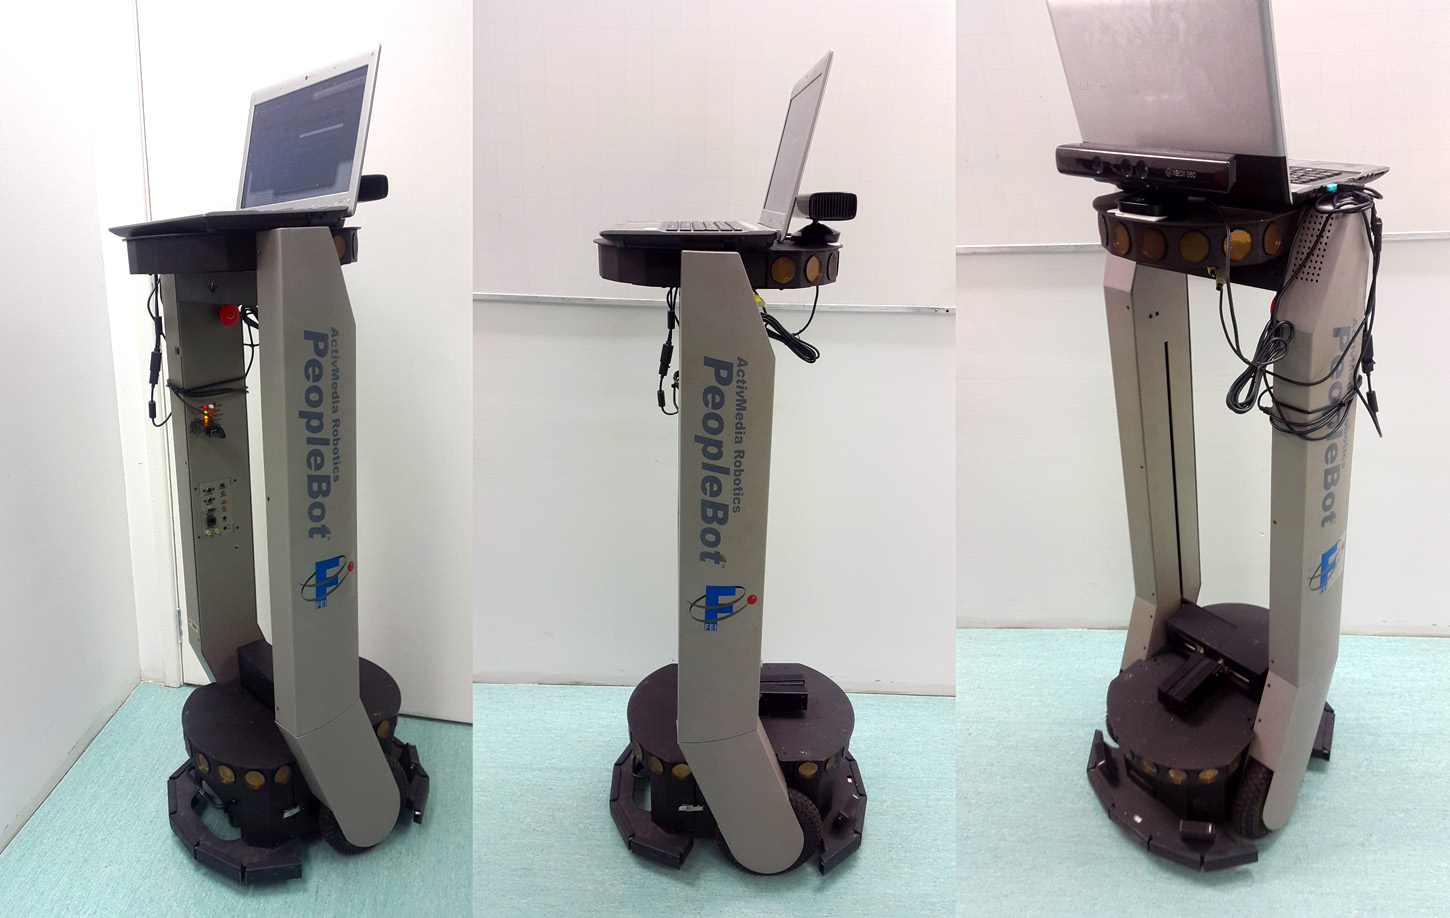
\includegraphics[width=\textwidth]{images/peoplebot.jpg}
	\caption{Robô ActivMedia Robotics PeopleBot.}
	\label{fig:peoplebot}
\end{figure}

Como a garra do PeopleBot é curta e não permite muitos movimentos, foi adicionado um manipulador para auxiliar na manipulação de objetos durante a interação com as pessoas e também na prestação de serviços domésticos e de cuidados pessoais. O projeto de construção do manipulador é apresentado através da figura~\ref{fig:manipulador}.

\begin{figure}[ht!]
	\centering
	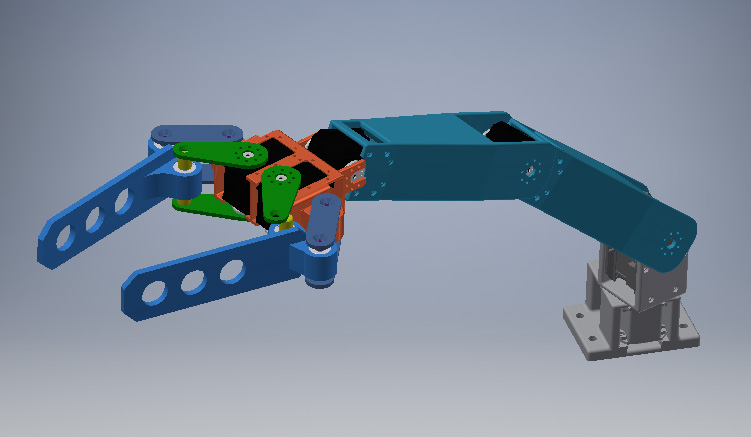
\includegraphics[width=0.6\textwidth]{images/manipulador.jpg}
	\caption{Projeto do Novo Manipulador do PeopleBot.}
	\label{fig:manipulador}
\end{figure}

O novo manipulador foi construído de maneira que os movimentos sejam parecidos com o braço humano. Além do manipulador, também será acoplado um \emph{tablet} para que seja possível atribuir faces ao robôs e deixar a interação mais amigável. Alguns sensores como o Microsoft\textregistered\ Kinect\textregistered\ e o ASUS\textregistered\ Xtion\textregistered\ também foram instalados para melhorar a captura das informações que são apresentadas na seção~\ref{sec:extracaocaracteristicas}, a seguir.

\section{Extração das Características para o RBC}
\label{sec:extracaocaracteristicas}

Como apresentado na seção \ref{cap:ihr}, existem diversas variáveis que podem auxiliar na extração de um perfil comportamental do individuo. \emph{Proxemics} tornam possível a extração de fatores sobre a distância social entre o individuo e o robô. Esses fatores podem variar não só entre a posição física dos dois agentes, mas também na posição do corpo dos indivíduos, como por exemplo, a orientação dos ombros e troco em relação a posição do robô. Outro fator também significante é a fixação entre olhares, este pode determinar o início e o fim de uma interação, além dos principais indivíduos na interação. Além disso, pode ser também empregado o reconhecimento de expressões faciais que auxiliam na análise do quanto a situação é confortável para o individuo, ou seja, o quanto ele está apreciando a interação, de tal forma, que possa existir uma avaliação em tempo real das reações deste durante todo o processo de interação. Outra técnica que pode ser utilizada na análise do conforto do individuo durante a interação é a avaliação da emoção através da voz da pessoa.

Dessa forma, é possível empregar diversos sensores que auxiliam a leitura e quantificação dessas variáveis. Sensores de captura de marcações de movimento, como Microsoft\textregistered\ Kinect\textregistered\ ou o ASUS\textregistered\ Xtion\textregistered, são utilizados para quantificar os valores obtidos através da \emph{Proxemic}, que envolvem distância entre agentes e orientação de membros do individuo. Para realizar o reconhecimento de expressões faciais utiliza-se uma câmera de video, podendo assim executar uma leitura da face do individuo em tempo de execução na interação entre o humano e o robô. As variáveis referentes a questão da fixação dos olhares dos agentes para identificar o início e o fim da interação, podem ser obtidas através de ambos sensores de tal forma, que seja possível determinar a orientação da cabeça e torso do individuo e também a direção do olhar deste para com o robô. A voz do individuo para análise da emoção na interação é obtida através de um microfone. A figura \ref{fig:capturacaracteristicas} apresenta a ilustração do processo de extração das características do individuo.

\begin{figure}[ht!]
	\centering
	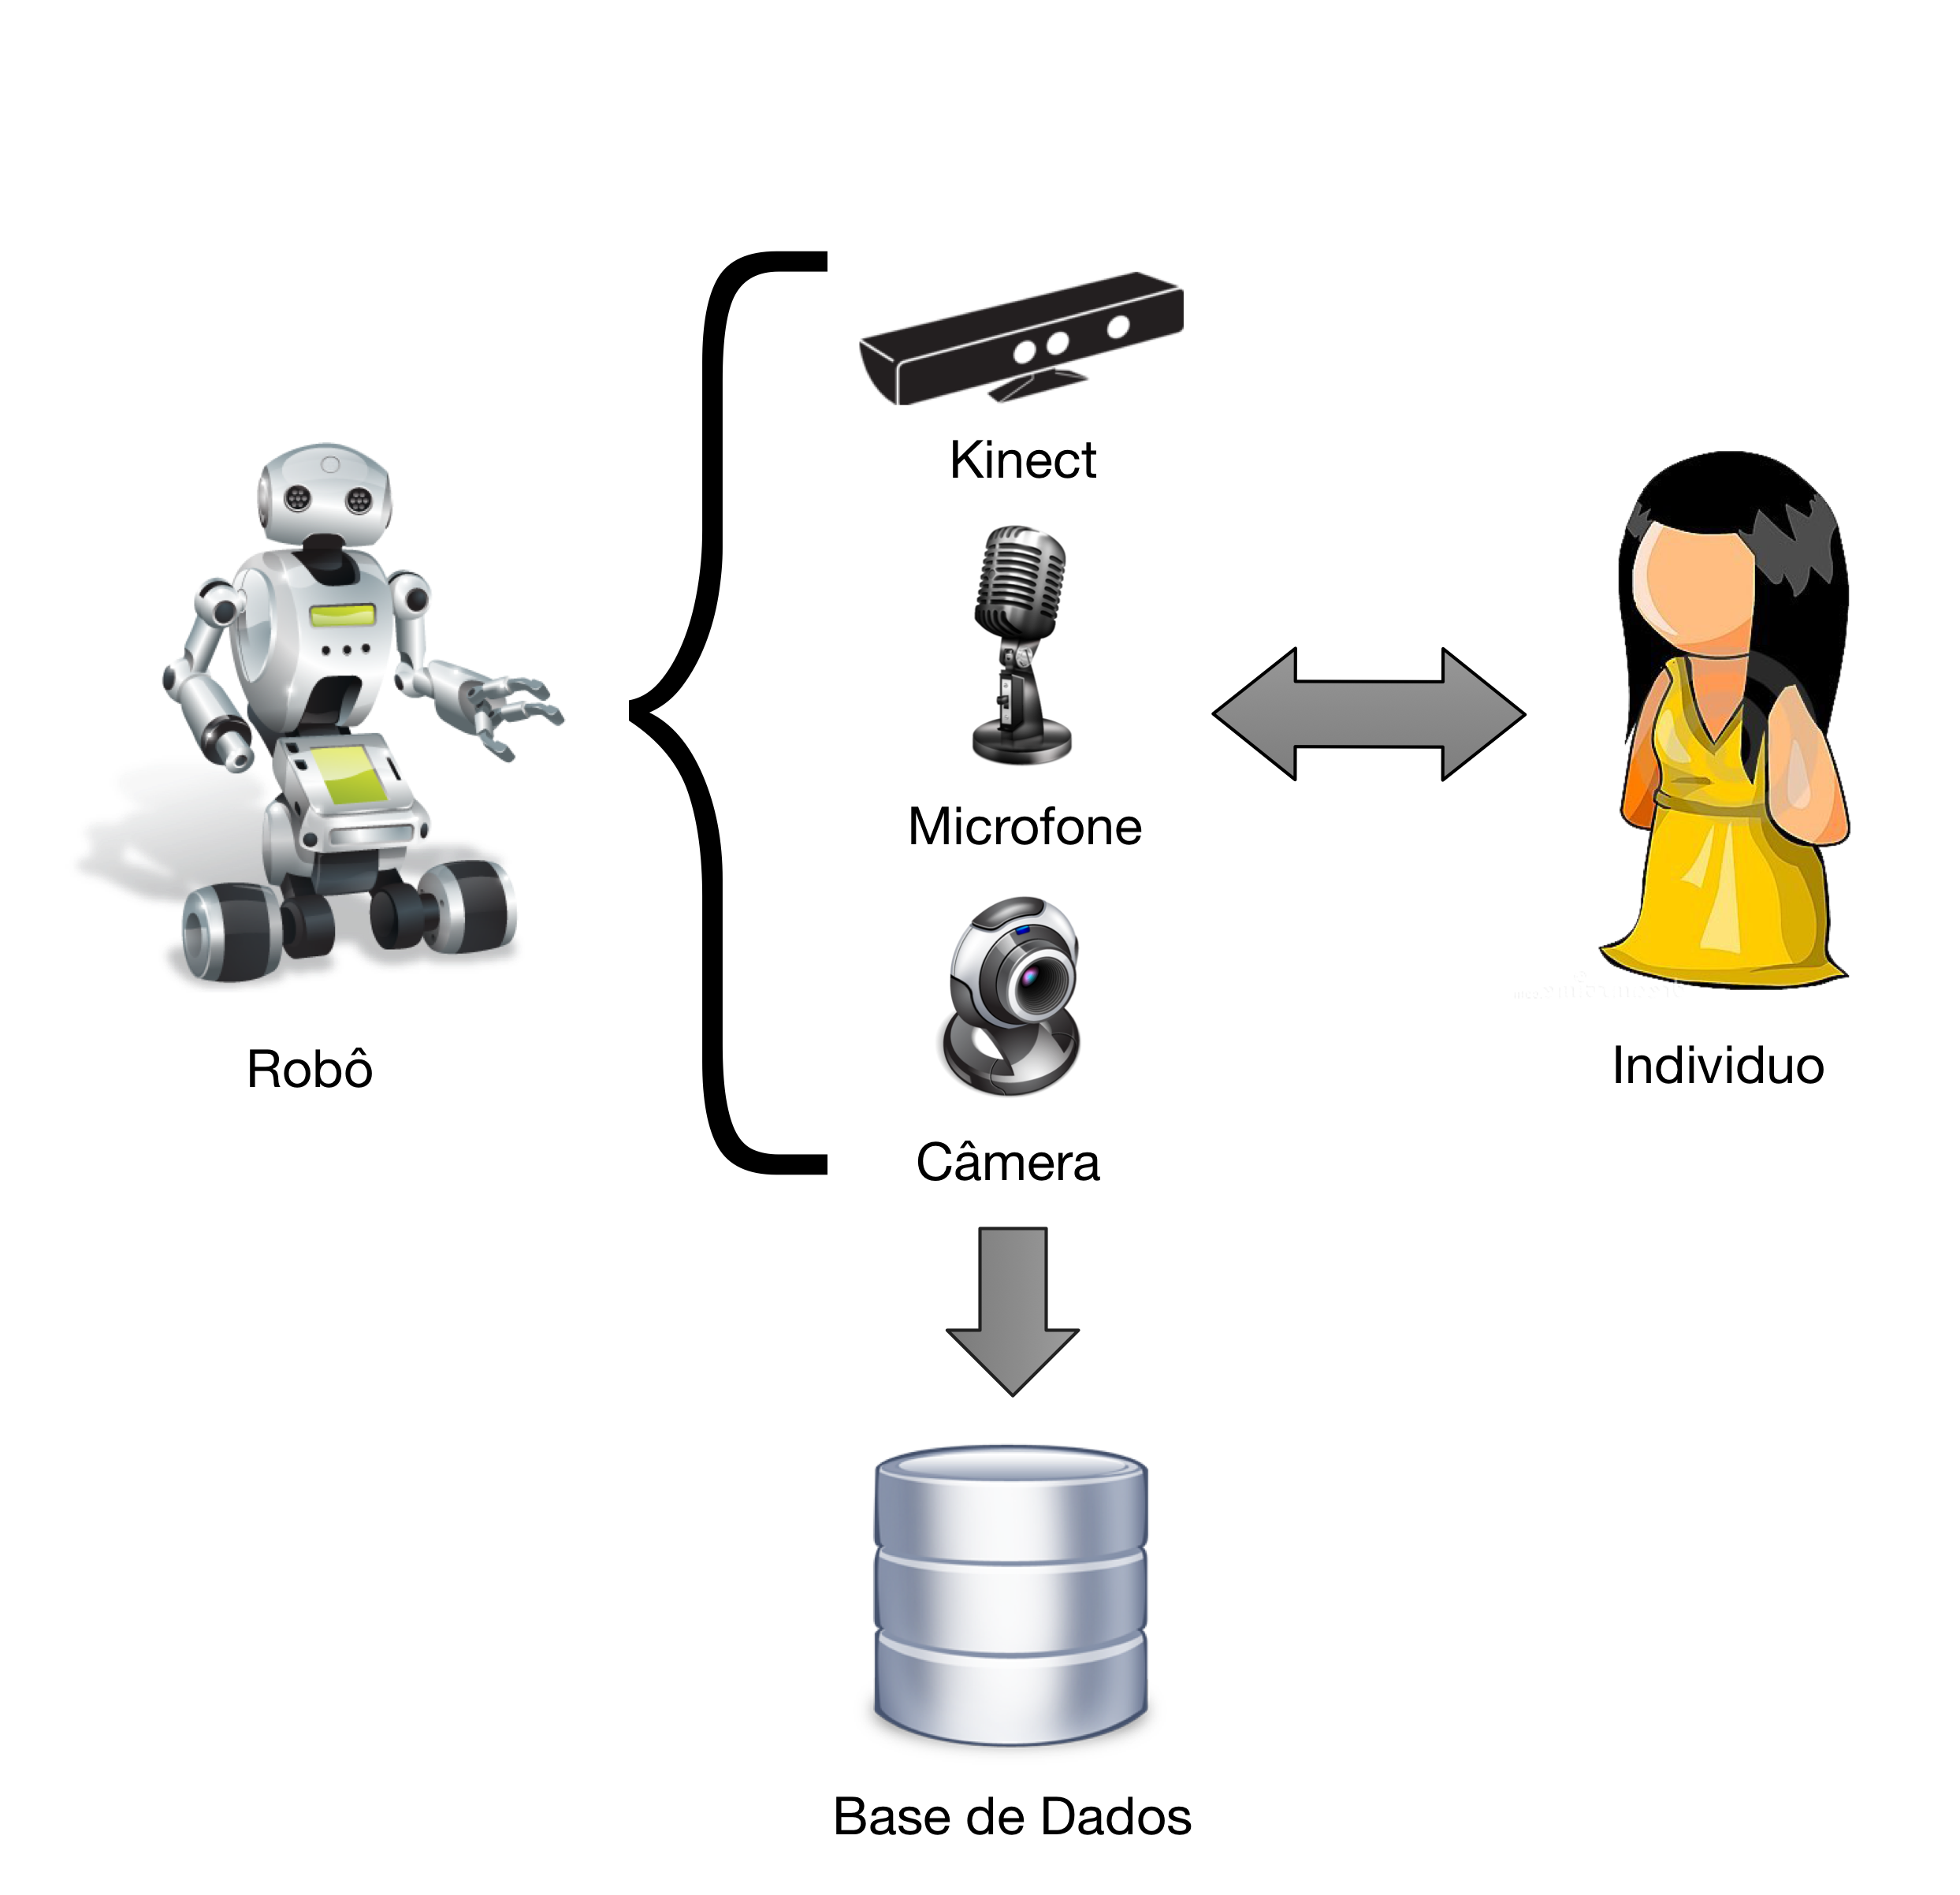
\includegraphics[scale=0.6]{images/captura_carac_individuo.png}
	\caption{Processo para a extração das características do individuo.}
	\label{fig:capturacaracteristicas}
\end{figure}

No processo apresentado pela figura \ref{fig:capturacaracteristicas}, o robô utiliza os sensores para identificar que o individuo iniciará uma interação com ele. Ao estabelecer o processo de interação, o robô utiliza um componente de \emph{log} que armazena todos os valores das variáveis que são utilizadas para determinar o perfil comportamental do individuo em um banco de dados. As variáveis são apresentadas em detalhes nas seções \ref{sec:variaveisindividuo} e \ref{sec:variaveisrobo}. Com as informações armazenadas determina-se através de um algoritmo de agrupamento, grupos que possuem perfis comportamentais similares, coletados e armazenados no banco de dados. Deve-se lembrar que as informações sobre o comportamento do individuo são direcionadas por um cenário de interação, como discutido por \citeonline{Jung:1991} em seu trabalho. 

Dessa forma, as variáveis aplicadas ao comportamento tem dependência do cenário de interação, porém as informações das variáveis etnográficas como idade, experiência computacional, sexo, local de origem, etnia, entre outras, são independentes do cenário. Existem alguns algoritmos na área de visão computacional que são capazes de identificar algumas variáveis etnográficas de maneira automática \cite{Yang:2007, Shan:2012, Ylioinas:2012, Samadi:2013, Amaral:2014}, porém para o trabalho desta tese, a coleta dessas informações será realizada através de um questionário pré interação já que esses algoritmos não fazem parte do objetivo principal do trabalho. As informações obtidas através do questionário serão inseridas no banco de dados complementando as informações de comportamento, que são separadas obtidas através da interação entre o ser humano e o robô através dos cenários de interação.

Na seção \ref{sec:variaveisindividuo} são detalhados os conjuntos de variáveis etnográficas e comportamentais com uma breve explicação dos objetivos esperados de cada uma das variáveis coletadas. A seção \ref{sec:variaveisrobo} detalha as variáveis que serão consideradas para o perfil do robô, apresentando também uma explicação sobre os objetivos de cada uma das variáveis.

\subsection{Selecionando as Variáveis para o Individuo}
\label{sec:variaveisindividuo}

Essa seção apresenta os conjuntos de variáveis que são consideradas nesse trabalho como a base de informações para seu desenvolvimento. Dois conjuntos são apresentados, o conjunto de variáveis etnográficas, seguido pelo conjunto de variáveis comportamentais que é o principal foco deste trabalho.

\subsubsection{Conjunto de Variáveis Etnográficas}
\label{sec:variaveisetnograficas}

O objetivo das variáveis etnográficas é identificar qual a experiência social e computacional de cada indivíduo. Além da experiência, também pode-se obter informações sobre a idade, gênero, local de nascimento ou origem do indivíduo. Todas essas informações são relevantes para verificar a existência de uma possível relação entre as variáveis etnográficas e comportamentais. A lista apresentada a seguir define as variáveis etnográficas e uma breve explicação sobre o significado de cada uma das variáveis.

\begin{enumerate}
	\item \textbf{Idade}: informa a idade do indivíduo.
	\item \textbf{Gênero}: informa o sexo biológico do indivíduo.
	\item \textbf{Local de Nascimento}: informa qual o local de nascimento do indivíduo. Essa variável auxiliará a determinar a base cultural do indivíduo.
	\item \textbf{Etnia}: informa a origem da família do indivíduo. Outra variável que auxilia na determinação da base cultural do indivíduo.
	\item \textbf{Quantidade de \emph{Gadgets}}: informa a quantidade de \emph{gadgets} que o indivíduo possui, ajudando a identificar qual a experiência e o contato dele com a tecnologia.
	\item \textbf{Contato prévio com Robôs}: informa apenas se o indivíduo já possuiu algum contato com robôs. Auxiliará a determinar o contato com a tecnologia, principalmente com robôs que poderá influenciar no seu comportamento durante a interação.
	\item \textbf{Tipos de Robôs}: informa quais são os tipos de robôs que o indivíduo teve contato. Os tipos poderão ser robôs \emph{Pet}, Humanoides, Androides, Móveis, entre outros. Essa variável é um complemento da variável ``Contato prévio com Robôs''.
	\item \textbf{Quantidade de cidades visitadas}: informa a quantidade de cidades que o indivíduo já visitou além da sua cidade natal. É importante para identificar o contato com outros tipos de cultura. Isso poderá influenciar no comportamento definido por sua cultura.
	\item \textbf{Quantidade de cidades que morou}: informa a quantidade de cidades que o indivíduo já morou além da sua cidade natal. É importante para identificar a vivência com outros tipos de cultura. Isso poderá influenciar no comportamento definido por sua cultura.
	\item \textbf{Quantidade de países visitadas}: informa a quantidade de países que o indivíduo já visitou além da sua cidade natal. É importante para identificar o contato com outros tipos de cultura. Isso poderá influenciar no comportamento definido por sua cultura.
	\item \textbf{Quantidade de países que morou}: informa a quantidade de países que o indivíduo já morou além da sua cidade natal. É importante para identificar a vivência com outros tipos de cultura. Isso poderá influenciar no comportamento definido por sua cultura.
\end{enumerate}

Em diversos trabalhos da seção \ref{sec:proxemicsihr}, onde a questão cultural do indivíduo é abordada, são discutidos que influência dela sobre o comportamenteo do o indivíduo. Contudo, a cultura é tratada como a origem do indivíduo, por exemplo, no trabalho de \citeonline{Eresha:2013}. Entretanto, a questão cultural na vida de uma pessoa é mais abrangente, está relacionada a experiência adquirida ao longo de sua vivência social. Dessa forma, o conjunto de variáveis apresentado acima tem como objetivo mapear de forma abstrata a experiência social do indivíduo, com o intuito de tornar o comportamento menos dependente da origem e talvez de sua experiência prévia.

Nesse trabalho, as informações levantadas nessa seção serão adquiridas através de questionários pré testes de interação. Em trabalhos futuros serão feitos estudos para identificar essas informações de maneira interativa através do próprio robô.

\subsubsection{Conjunto de Variáveis Comportamentais}
\label{sec:variaveiscomportamentais}

Variáveis comportamentais tem como principal objetivo identificar o comportamento do indivíduo. Nesse trabalho o comportamento está diretamente relacionado com cenários de interação social. As variáveis comportamentais são coletadas a partir de informações sobre as posições corporais e expressões faciais do indivíduo, tornando possível uma análise com base em teorias de linguagem corporal. As análises realizadas a partir da linguagem corporal, tem por base o trabalho apresentado por \citeonline{Lambert:2008}. O conjunto de variáveis comportamentais apresentados nessa seção não são utilizadas apenas para extrair o perfil do indivíduo, mas também para avaliar se a ação realizada pelo robô gerou uma reação positiva ou negativa no indivíduo. A lista apresentada a seguir define as variáveis comportamentais e uma breve explicação sobre o objetivo de cada uma das variáveis.

\begin{enumerate}
	\item \textbf{Expressões Faciais}: é possível identificar se a reação do indivíduo foi positiva ou negativa, a partir de uma ação do robô. Existem seis expressões bases que combinadas formam diversas outras~\cite{Bihan:2014}. Contudo, nesse trabalho será considerado apenas as seis expressões bases classificadas em dois grupos: expressões faciais positivas e expressões faciais negativas. O intuito dessa variável é realizar a avaliação da ação do robô com base nas expressões faciais do indivíduo.
	\item \textbf{Tempo de Transição entre as Zonas Sociais}: identificar o tempo que o indivíduo ficou confortável com a presença do robô a medida que esse diminuiu a distância entre eles.
	\item \textbf{Frequência do Olhar em direção ao Robô}: identificar se o indivíduo mantém o olhar ao robô, sendo possível saber se a interação está continua ou não. Isso pode influenciar se o robô está interagindo de maneira confortável ao indivíduo ou se esse está incomodado com a presença do robô.
	\item \textbf{Tempo do Olhar}: é possível mensurar o interesse do indivíduo durante a interação através do tempo que ele permanece com o olhar fixo no robô. Quanto maior o tempo do olhar, maior o interesse na interação do indivíduo.
	\item \textbf{Orientação dos ombros}: Auxilia a mensurar o interesse do indivíduo durante a interação, analisando se os ombros possuem a mesma orientação que a cabeça e também uma orientação em direção ao indivíduo que interage com o robô. Além disso, é possível determinar através do alinhamento do quadril com o ombro do indivíduo o ângulo de inclinação de seu torso. A inclinação do torso auxilia a identificar o interesse do indivíduo na interação, para isso basta verificar se ele está inclinado em direção ao robô para determinar um interesse positivo.
	\item \textbf{Orientação do quadril}: Auxilia a mensurar o interesse do indivíduo durante a interação. A orientação do quadril em direção ao robô ou na direção oposta auxilia a determinar o grau de interesse do indivíduo na interação. Quando mais alinhado à direção do robô, maior o interesse do indivíduo na interação.
	\item \textbf{Estilo da Voz}: é importante, pois pode determinar a reação que o indivíduo terá após a interação via áudio com o robô. Além disso, é possível determinar se o indivíduo está confortável ou não durante a interação, analisando o tom de sua voz ao responder o robô. Nesse trabalho, será considerado somente o canal de resposta ao indivíduo. A análise do tom da voz do indivíduo não será considerado nesta tese e ficará para trabalhos futuros de aprimoramento do componente de análise comportamental em IHR.
\end{enumerate}

\subsection{Selecionando as Variáveis para o Robô}
\label{sec:variaveisrobo}
Além das variáveis referentes ao perfil do indivíduo, deve-se considerar também as informações sobre o robô uma vez que sua aparência pode influenciar na reação das pessoas durante a interação~\cite{Hegel:2009}. Coletar as variáveis do robô pode auxiliar a identificar quais são os principais fatores que tornam a interação humano-robô desconfortável ou com menos qualidade. Dessa forma, foi definido um conjunto de variáveis que pudessem caracterizar da melhor maneira fatores do robô, referente a sua aparência, que influenciam na IHR. Esse conjunto de variáveis é apresentado a seguir:

\begin{enumerate}
	\item \textbf{Altura}: A altura do robô para identificar a influência da diferença entre alturas de robôs e humanos.
	\item \textbf{Volume}: O volume ocupado pelo robô pode influenciar no conforto da interação, uma vez que quando o robô atingir uma zona social mais próxima do indivíduo pode causar uma sensação claustrofóbica a ele.
	\item \textbf{Tipo do Robô}: Segundo \citeonline{Choi:2014}, robôs possuem dois tipos: Autônomos e Tele-operados. Essa variável define o quanto de intervenção humana é necessário para que o robô possa executar a tarefa objetivo.
	\item \textbf{Classificação do Robô}: Segundo \citeonline{Dobra:2014} classificar um robô é uma tarefa muito complexa e pode envolver diversas variáveis. Dessa forma, para essa tese será considerado uma classificação mais simples. O robô deve ser classificado como: fixo, móvel com rodas, móvel bípede, móvel quadrupede, móvel com manipuladores. Outras classificações podem ser inseridas conforme a necessidade e inclusão de novos robôs.
	\item \textbf{Aparência Física}: Essa variável descreve se o robô possui uma aparência amigável ou agressiva.
	\item \textbf{Nível de Ruído}: Determina qual o nível de ruído que os atuadores do robô podem gerar de tal forma, que possa influenciar na interação humano-robô.
\end{enumerate}

Além das variáveis que definem as características, é necessário também o mapeamento das ações que o robô irá executar para que exista uma avaliação dessa após a reação do indivíduo. As variáveis que compõem as informações do perfil comportamental do robô são:

\begin{enumerate}
	\item \textbf{Aproximação}: Forma de aproximação do robô ao indivíduo. Pode ser classificada entre rápida, devagar, brusca ou suave.
	\item \textbf{Movimentação do Manipulador}: Caso exista um manipulador deve descrever como é feita a movimentação do manipulador em direção ao usuário. A classificação consiste em brusca ou suave.
	\item \textbf{Estilo de Voz}: Ao emitir algum tipo de som o robô deverá manter um estilo de voz para que seja possível simbolizar qual o tipo de mensagem ele deseja falar. A classificação será feita de maneira simplificada, considerando apenas se é um estilo educado ou agressivo.
	\item \textbf{Expressão Facial}: Ao iniciar o contato visual com o indivíduo, pode ocorrer diversas expressões do robô na tentativa de manter o conforto do indivíduo durante o processo de interação. Simplificando as expressões, de maneira similar ao apresentado na seção~\ref{sec:variaveiscomportamentais}, são consideradas apenas dois tipos de expressões realizadas pelo robô: amistoso e não-amistoso. As expressões faciais do robô serão executadas através do \emph{tablet} acoplado nele, conforme descrito na seção~\ref{sec:robo}.
\end{enumerate}

As variáveis comportamentais do robô definidas com o objetivo de executar uma tarefa de abordagem para estabelecer uma interação. Caso seja necessário adicionar novas variáveis a esse conjunto não haverá problema ao método apresentado ao longo da seção.

\section{Raciocinando com Base nas Interações Extraídas}
\label{sec:raciociniointeracao}

Com as variáveis comportamentais e etnográficas do indivíduo e do robô definidas é necessário definir o método que fará com que o robô seja capaz de aprender a interagir com seres humanos a partir das suas experiências passadas. No capitulo \ref{cap:rbc} foi apresentado a técnica de Raciocínio Baseado em Casos (RBC) que tem como principal objetivo o desenvolvimento de um sistema de conhecimento com base em experiências ou casos ocorridos anteriormente. RBC tem uma estrutura baseada em 4(quatro) pilares, são eles~\cite{Lopez:2013}: Resgatar, Reutilizar, Revisar e Reter. A figura~\ref{fig:rbc} apresenta a metodologia dessa tese, que engloba as quatro etapas do RBC.

\begin{figure}[ht!]
	\centering
	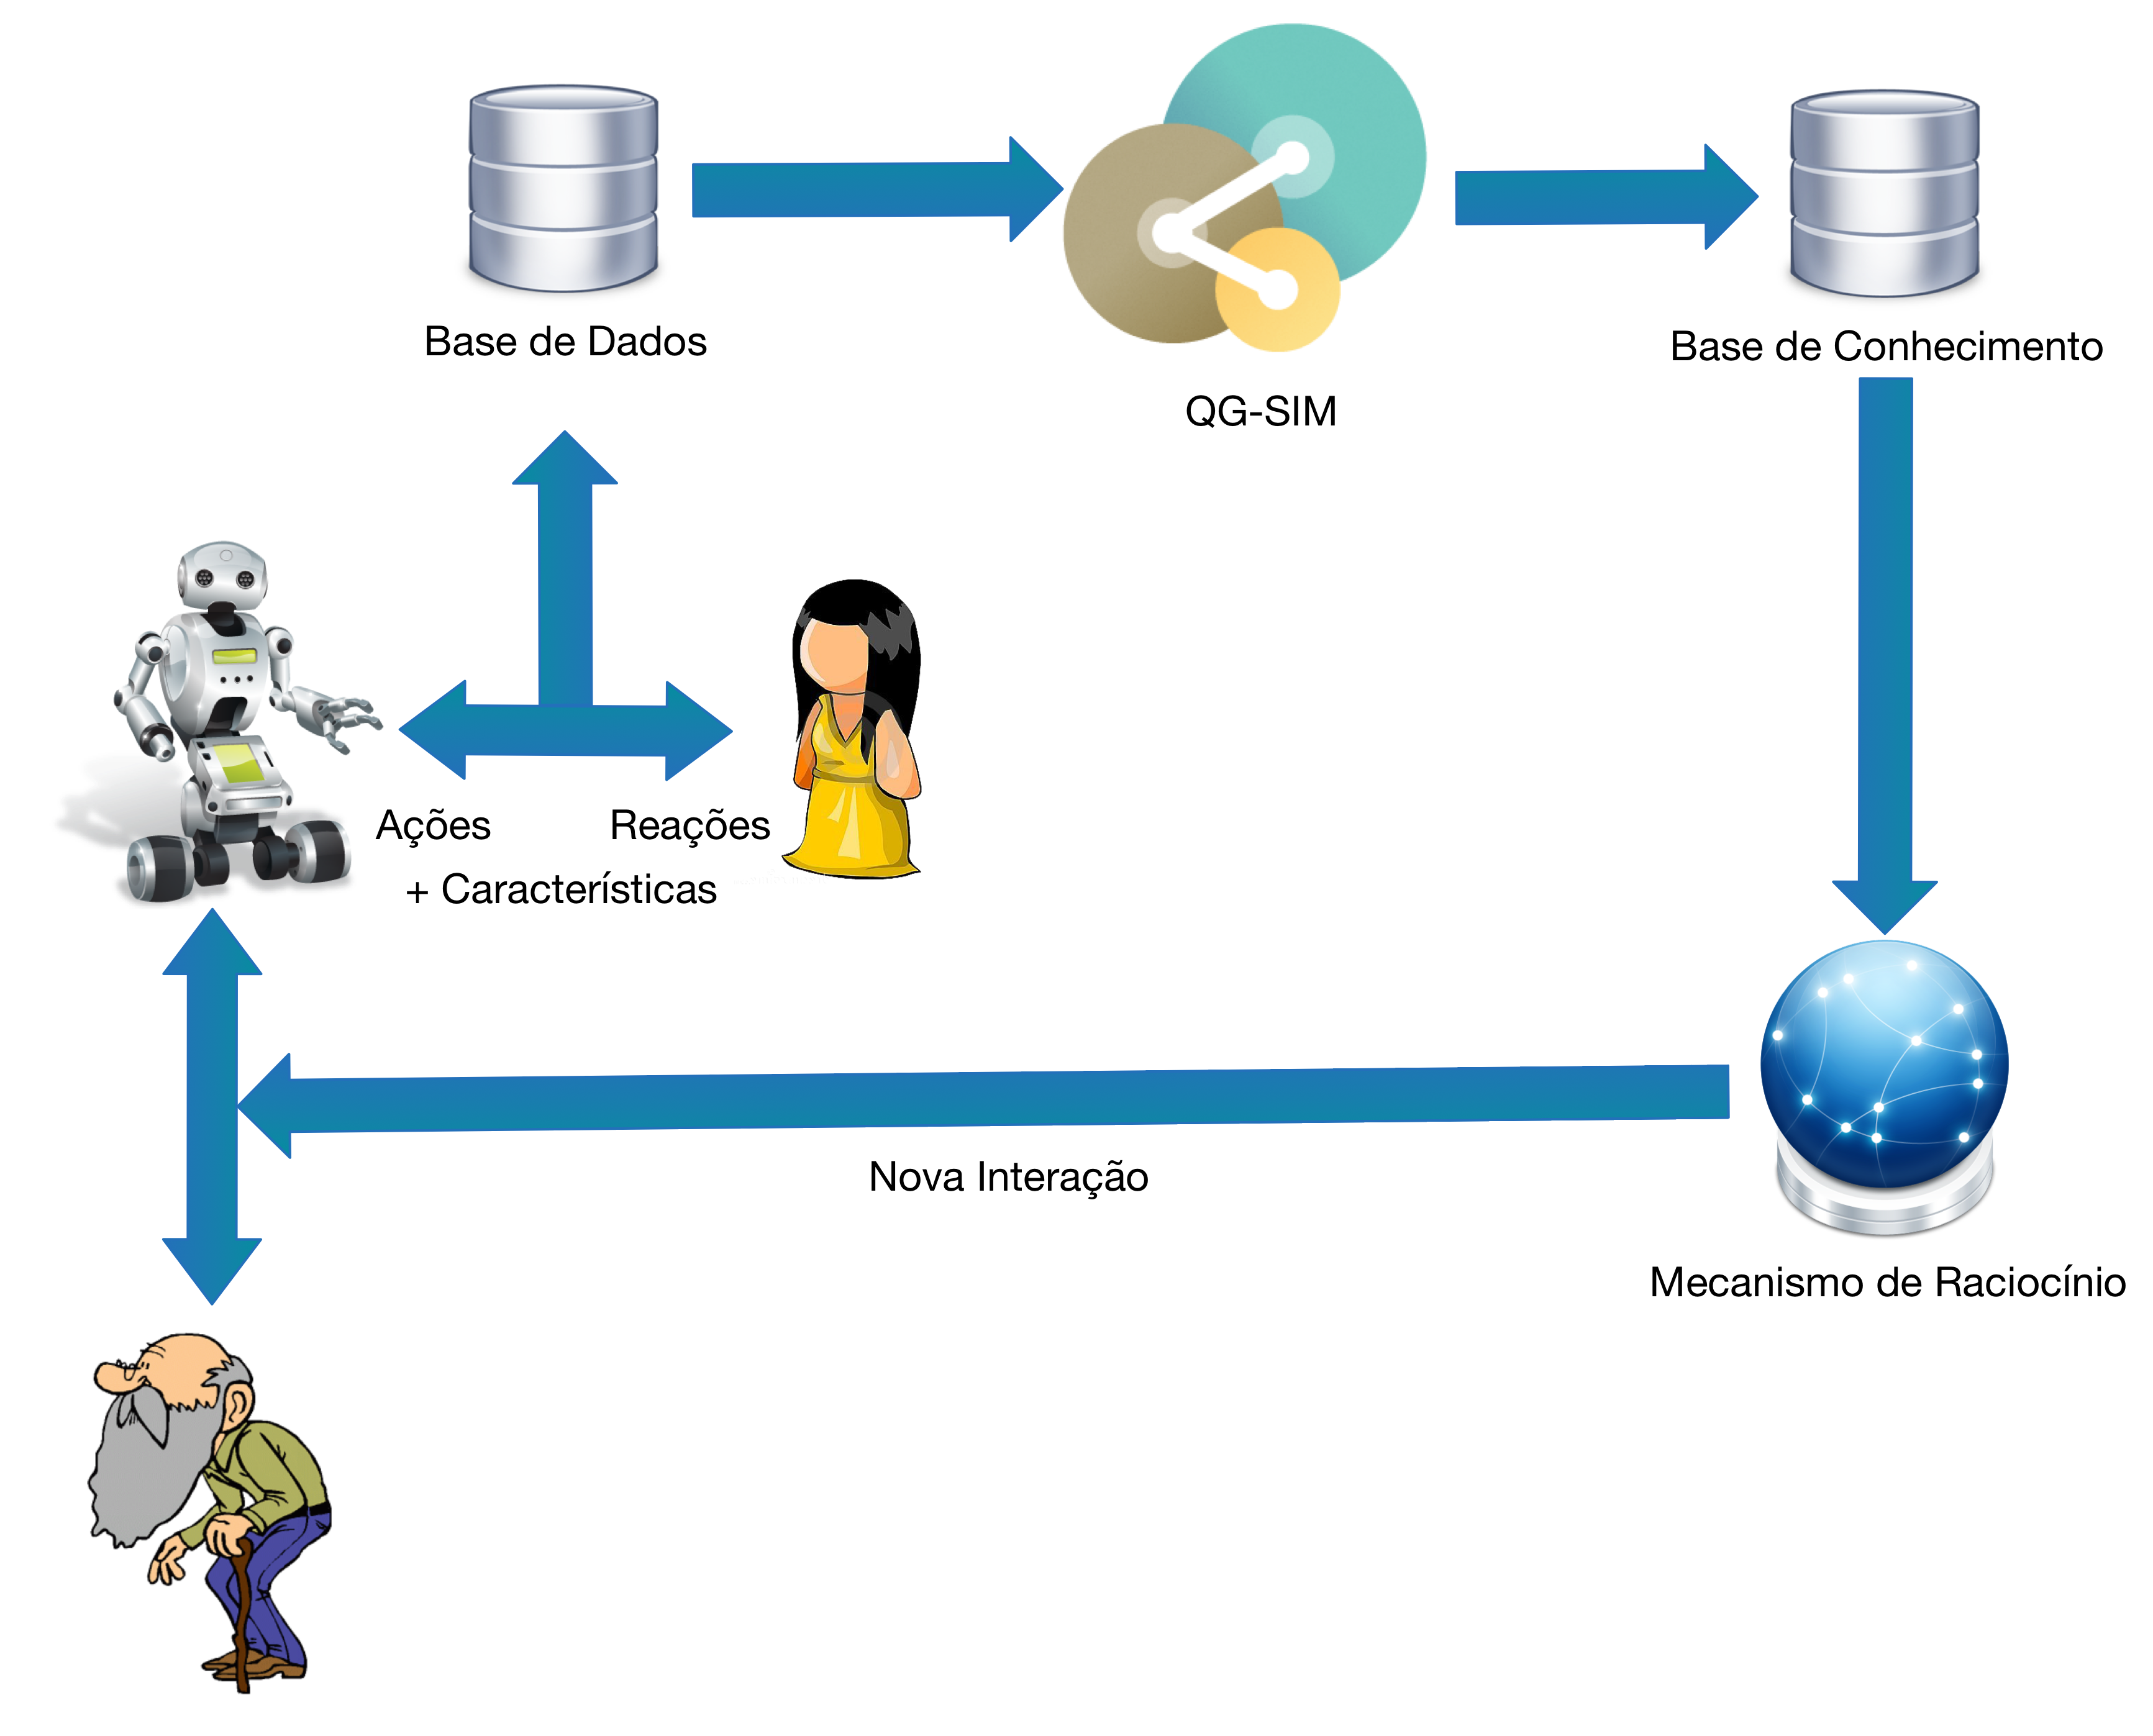
\includegraphics[width=\textwidth]{images/rbc_geral.png}
	\caption{Processo de Interação com Aprendizado baseado em Experiências Passadas.}
	\label{fig:rbc}
\end{figure}

A metodologia da figura~\ref{fig:rbc} tem início na interação entre o robô e a jovem localizada a sua frente. Durante a interação entre os dois o sistema coleta todas as reações da jovem para cada ação tomada pelo robô, de acordo com as variáveis descritas na seção~\ref{sec:extracaocaracteristicas}, que são armazenadas na base de dados. A base de dados formada a partir dessas informações é enviada ao algoritmo de agrupamento por similaridade QG-SIM (Quality Groups of Similarity, em inglês)~\cite{Masiero:2013}. Os grupos gerados pelo QG-SIM são analisados e inseridos na base de conhecimento formando os casos de pesquisa para novas interações. Quando ocorrer uma nova interação, como por exemplo o robô com o senhor na figura~\ref{fig:rbc}, o mecanismo de raciocínio realiza uma análise para que possa inferir qual o melhor caso a ser aplicado para interação entre o senhor e o robô. Mesmo que utilize casos existentes na base de conhecimento, todas as interações são armazenadas para manter o aprendizado sobre interações contínuo e sempre com o objetivo de manter o individuo confortável durante todo o processo. Na sequência serão detalhadas as fases do RBC de acordo com a metodologia apresentada na figura~\ref{fig:rbc}.

\subsection{Resgatar}
\label{sec:resgatar}

A partir de uma nova interação inicia-se o processo de resgate do caso que maximize as reações positivas de um determinado indivíduo a partir da ação que o robô realiza. Nessa fase a solução encontrada não poderá ser dada como exclusiva, pois quando trata-se de seres humanos a tarefa de determinar uma solução exata é complexa. Como para um mesmo perfil de indivíduo ou um perfil similar pode-se apresentar muitas soluções deve ser aplicado nessa fase um modelo probabilístico de tal forma, que a solução escolhida seja a que possui um maior valor de probabilidade no ponto de vista de maximizar a satisfação e o conforto do indivíduo.

Existem diversos métodos probabilísticos que podem ser aplicados nessa fase, como por exemplo, redes Bayesianas ou até mesmo conjunto de lógica nebulosa (Lógica \emph{Fuzzy}). Mesmo sendo o regaste de uma solução único para o caso, esse modelo possibilita que a solução selecionada para execução seja a melhor dentre todas as armazenadas dada uma distribuição probabilística. Selecionando o caso que será aplicado esse deve formar um conjunto de ações do robô para interação com o indivíduo, como é apresentado na próxima seção.

\subsection{Reutilizar}
\label{sec:reutilizar}

Após o resgate do caso que possui a maior similaridade de tornar a interação confortável ao indivíduo é necessário construir a sequência de ações que o robô irá executar. Para isso, deve-se considerar duas premissas. A primeira é que uma ação é dependente da anterior, pois caso essa premissa não seja considerada as ações que o robô executará não apresentarão nenhum sentido ao indivíduo. Isso faz com que esse modelo de reutilização seja considerado como temporal, onde uma ação futura depende de uma ação passada. A segundo premissa que deve ser considerada é que o indivíduo irá se comportar de maneira diferente da esperada em algum momento do processo de interação. Dessa maneira, deve-se realizar um novo resgate para a solução que maximiza o conforto da interação a partir daquele ponto onde a reação do indivíduo foi diferente do esperado.

\subsection{Reter}
\label{sec:reter}

Durante a interação entre o robô e um indivíduo as informações sobre o comportamento são armazenadas em um banco de dados. A partir desse banco de dados é realizado um agrupamento entre os perfis comportamentais que possuem uma certa similaridade. Para realizar esse agrupamento é utilizado um algoritmo chamado QG-SIM. O QG-SIM~\cite{Masiero:2013} mantém a qualidade da similaridade entre os perfis de um mesmo grupo, sendo dessa maneira, o algoritmo ideal para esse tipo de tarefa e cenário.

Com os grupos formados é utilizado uma processo definido por \citeonline{Masiero:2013} para gerar um perfil comum ao grupo. Esse perfil comum também pode ser considerado a centroide do grupo. O procedimento para encontrar a centroide do grupo auxilia a determinar o perfil que será inserido na base do conhecimento que é utilizada no processo de resgate e reutilização do sistema de RBC.

A opção de realizar esse processo de agrupamento para inserir um caso na base de conhecimento é importante, pois diminui a quantidade de casos para busca por parte do sistema de RBC. Diminuir o número de casos aumenta o desempenho do algoritmo fazendo com que o robô tenha uma resposta na interação mais rápida, evitando com que o indivíduo espere muito por uma ação do robô.

\subsection{Revisar}
\label{sec:revisar}

Com a base de conhecimento formada é executado um procedimento para verificar se existem perfis iguais ou similares a ponto que possam ser excluídos. Dessa maneira, é possível manter a base de conhecimento sempre com perfis exclusivos entre os existentes. Assim, é possível garantir que um número maior de indivíduos seja atendido pelo sistema de RBC.

Apesar da metodologia apresentada na figura~\ref{fig:rbc} possuir apenas um robô na interação, é possível transferir esse conhecimento a diversos robôs já que em sua arquitetura todo o sistema de RBC é extra robô. Assim, o processamento e conhecimento adquirido pelo sistema de RBC ficará disponível em um servidor ao qual todo robô que quiser utilizar dessas informações terá livre acesso.

Todo esse sistema será testado em um cenário de primeiro contato para interação entre dois agentes, nesse caso um robô e um indivíduo. O robô utilizado tem a locomoção feita através de rodas, porém sua altura é próxima da média dos seres humanos. As características do robô fazem com que ele seja apropriado para interações entre humanos e robôs.
% %!TEX root=Principal.tex
\chapter{CENÁRIOS DE TESTE}
\label{cap:testes}
Esse capítulo apresentará os cenários de teste considerados para auxiliar a validação do processo de aprendizado de interação entre humanos e robôs proposto por essa tese. São apresentados dois cenários, o primeiro representa a primeira abordagem para interagir com pessoas desconhecidas e o segundo cenário é uma continuação do primeiro, onde a partir de interações passadas o robô auxiliará uma pessoa durante alguma tarefa no ambiente doméstico.

\section{Cenário 1 - Primeira Interação}
\label{sec:cenario1}
O primeiro cenário de teste ocorre com o pressuposto de que o robô nunca interagiu com a pessoa em questão previamente. Para isso o robô PeopleBot é posicionado frente a frente com a pessoa. As informações sobre distância social(vide seção~\ref{sec:proxemics}) serão utilizadas para validar o cenário. A figura~\ref{fig:cenario1} apresenta uma ilustração do cenário e suas possibilidades.

\begin{figure}[ht!]
	\centering
	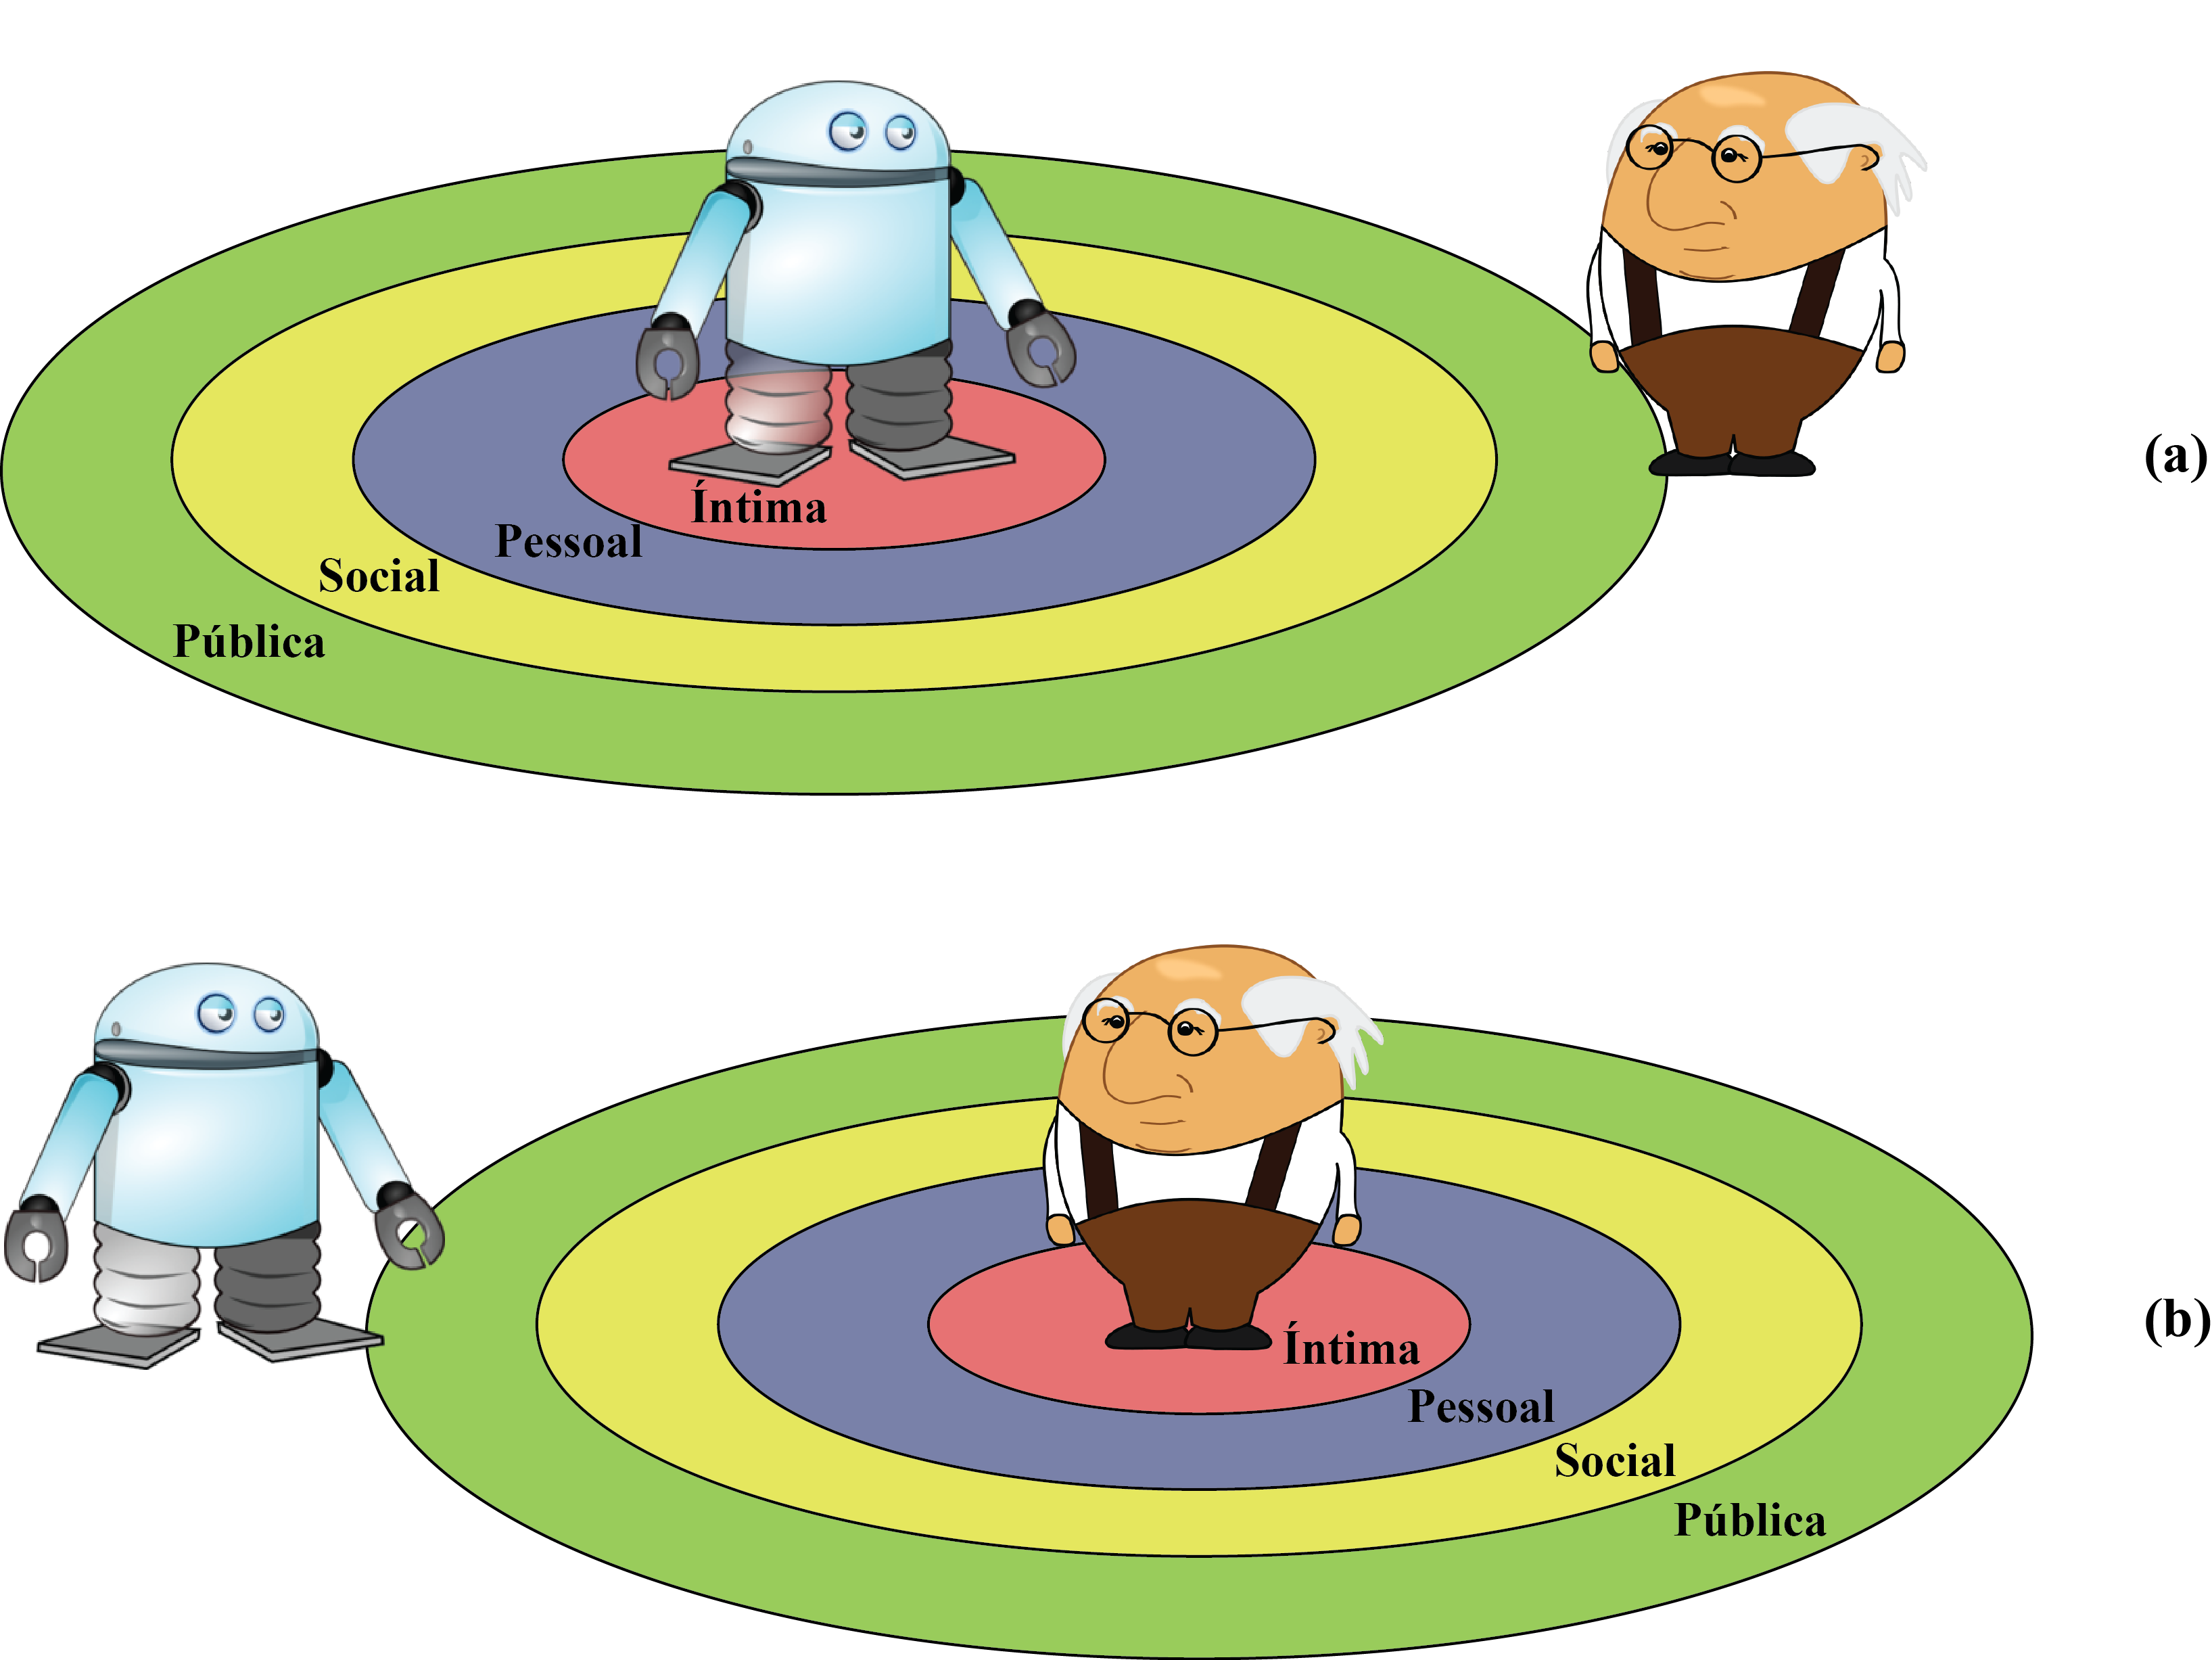
\includegraphics[width=0.8\textwidth]{images/cenario01.png}
	\caption{Cenário de teste para primeira interação entre humano e robô.}
	\label{fig:cenario1}
\end{figure}

Na figura~\ref{fig:cenario1}a o robô permanece parado e inicia a interação com a pessoa de tal forma, que essa sinta-se confortável e aproxime-se do robô. O cenário será considerado como concluído e também como sucesso quando a pessoa entrar pelo menos na zona pessoal do robô, demarcada pela cor azul, e permanecer pelo menos alguns segundos nela. A figura~\ref{fig:cenario1}b representa o cenário inverso. Nesse a pessoa fica parada e durante a interação o robô vai se aproximando dele. A velocidade que o robô irá se aproximar dependerá das reações positivas e negativas da pessoa para com as ações do robô. Como o cenário figura~\ref{fig:cenario1}a, o sucesso será determinado na entrada e permanência do robô à zona pessoal do indivíduo.

\section{Cenário 2 - Cenário Doméstico}
\label{sec:cenario2}
Nesse segundo cenário de teste o robô e a pessoa já interagiram previamente, sendo assim o desconforto inicial de interação já deve não existir mais. Contudo, variáveis como humor e tarefa a ser executada podem contribuir com a variação no estilo de interação. Dessa forma, o robô deve continuar com a preocupação de manter o ser humano confortável durante a execução da tarefa de ajuda. Para validar essa segunda interação é proposto um cenário de atividade doméstica, representado através da figura~\ref{fig:cenario2}.

\begin{figure}[ht!]
	\centering
	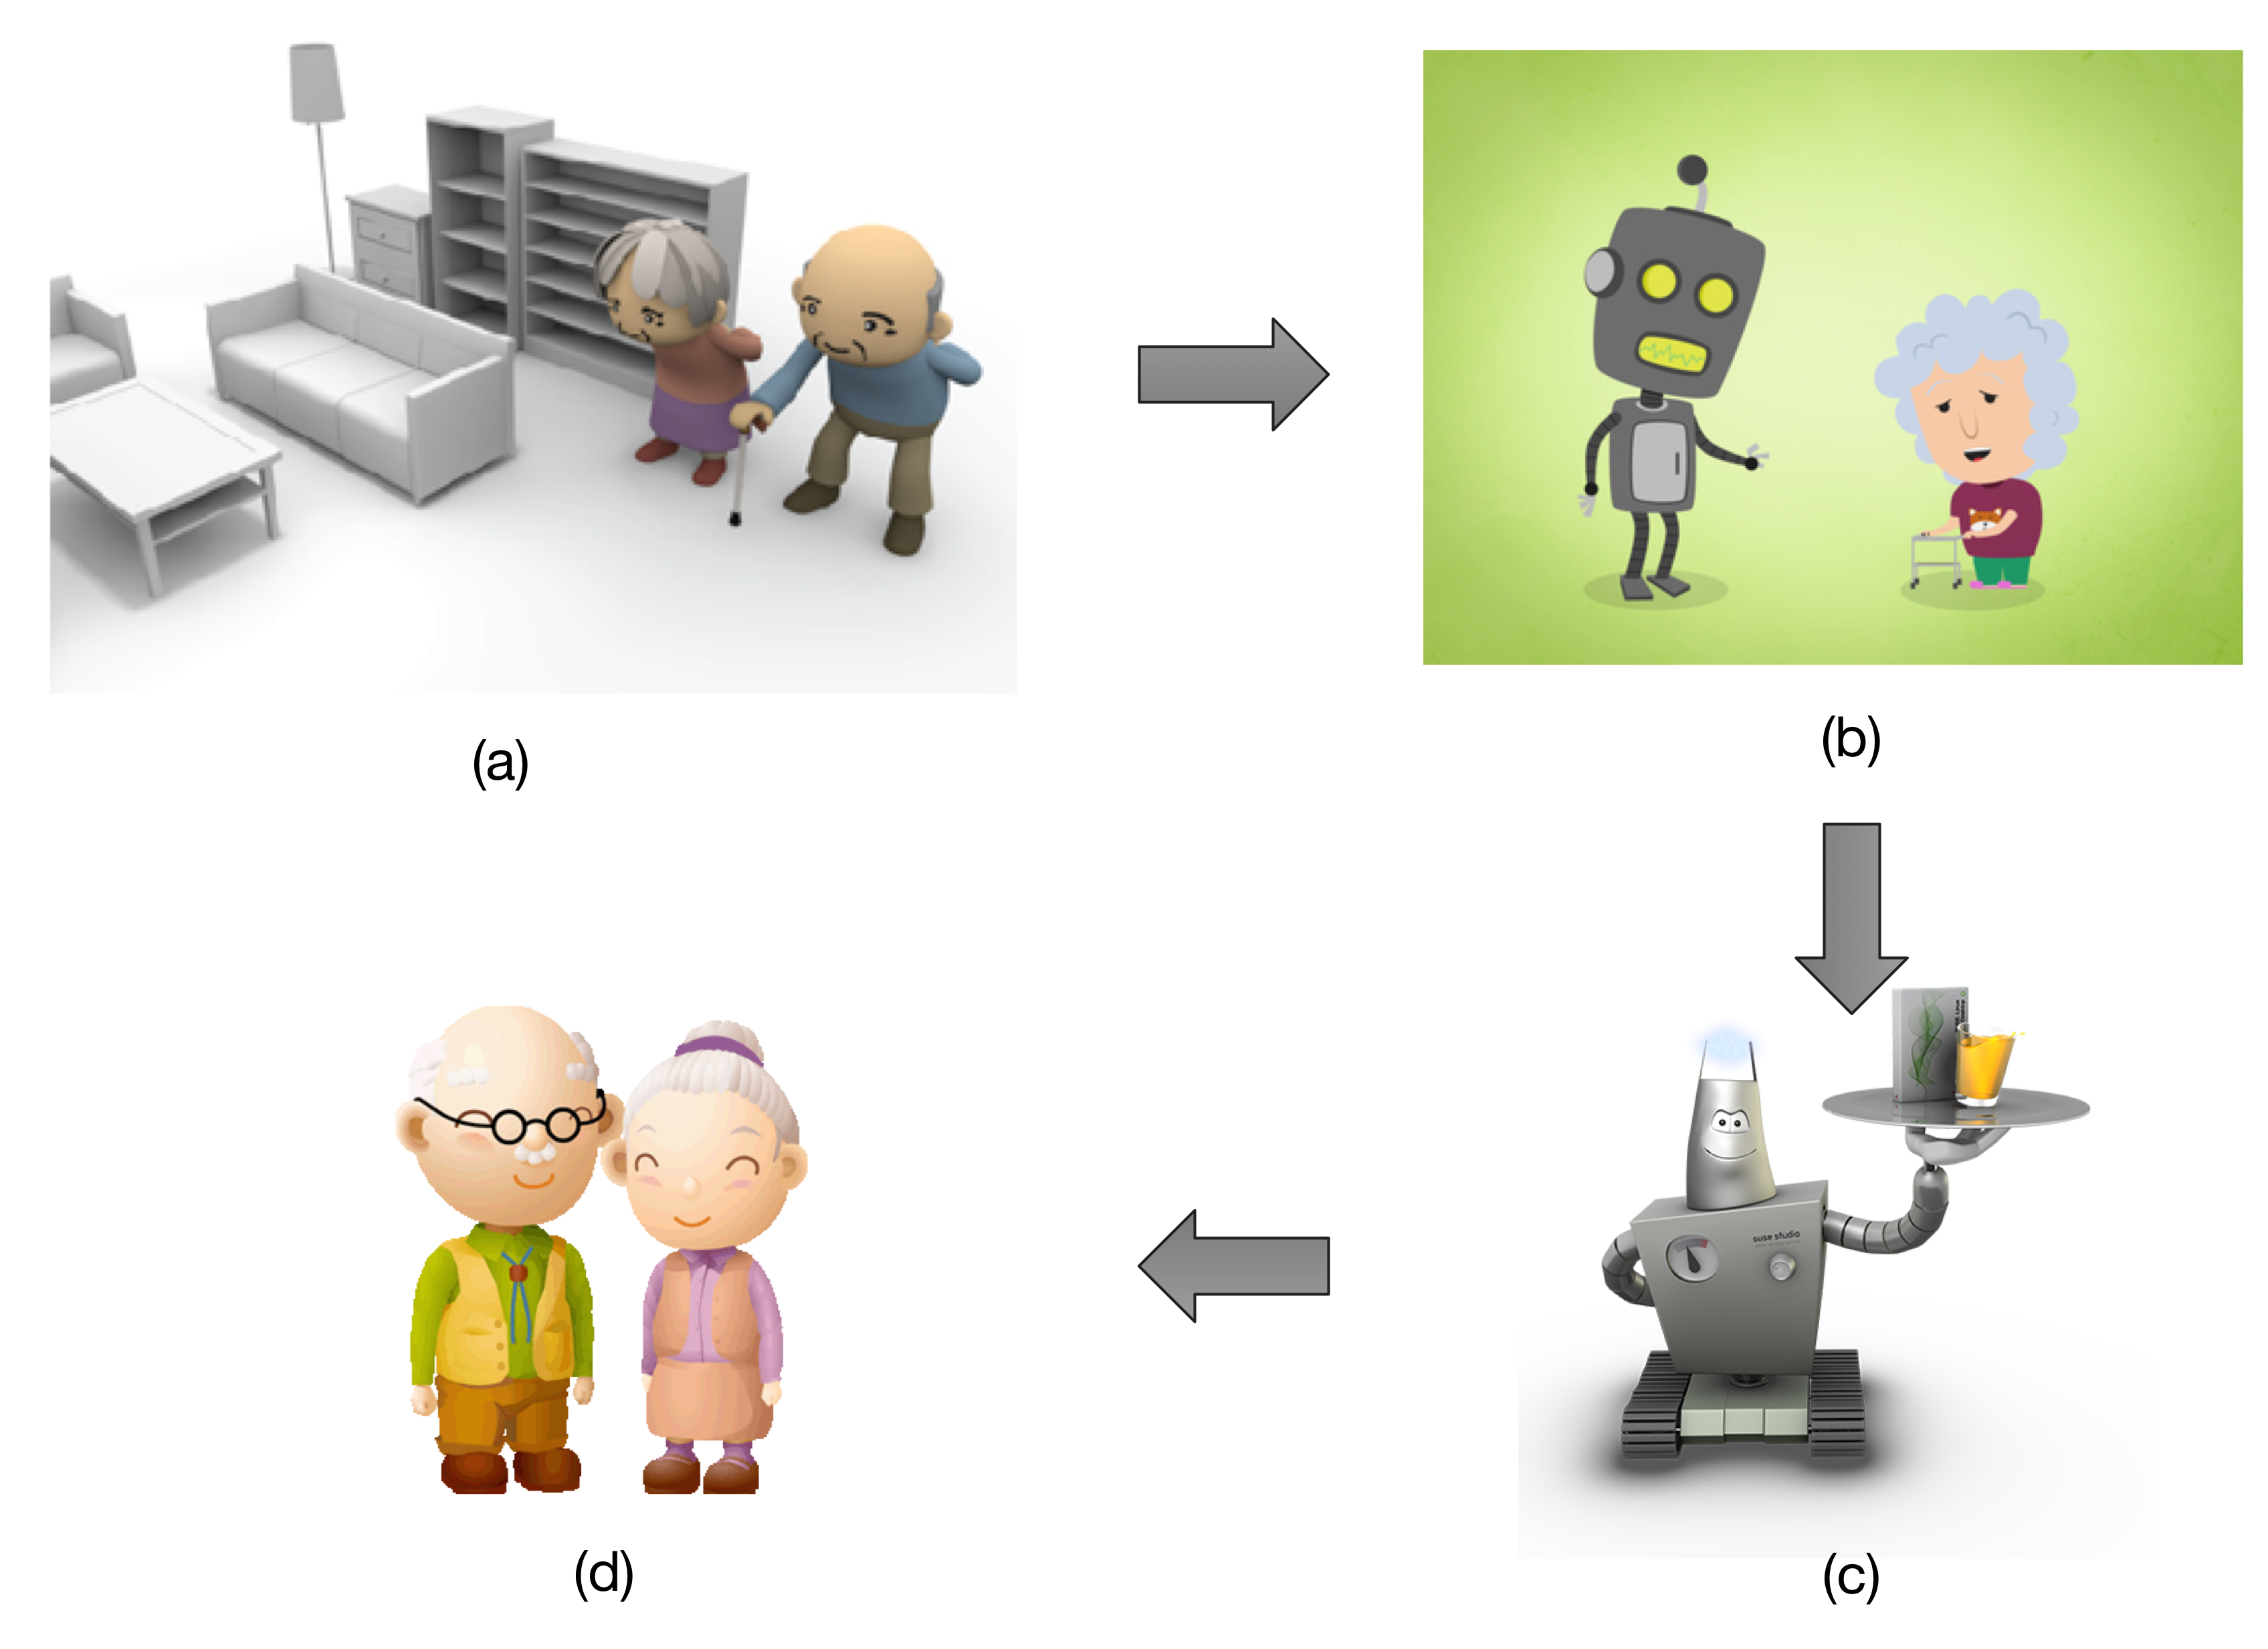
\includegraphics[width=0.8\textwidth]{images/cenario02.png}
	\caption{Cenário de teste para segunda interação entre humano e robô.}
	\label{fig:cenario2}
\end{figure}

O cenário apresentado na figura~\ref{fig:cenario2} é composto por quatro etapas, são elas: (a) existem pessoas em um ambiente doméstico e elas necessitam de alguma ajuda, seja para pegar um copo d'água ou tomar um medicamento, solicitando ao robô através de um comando de voz; (b) o robô percebe através de um movimento brusco da pessoa utilizando os sensores do Microsoft\textregistered\ Kinect\textregistered\ ou o ASUS\textregistered\ Xtion\textregistered\ ou recebe a informação direta através de um comando de voz pela pessoa solicitando a ajuda. O robô se aproxima do indivíduo de acordo com as informações obtidas e processadas a partir do cenário~\ref{sec:cenario1}. Ele também se mantém atento para qualquer adaptação de comportamento que seja necessário durante a interação alimentando a base de dados; (c) o robô identifica a ajuda que lhe foi solicitada e realiza a tarefa de acordo com o solicitado e na sequência retorna até a pessoa que lhe solicitou a ajuda; e (d) por fim, a pessoa que recebeu ajuda esboça o seu contentamento para com o robô pelo serviço prestado através de um elogio verbal, uma expressão facial positiva (sorriso, por exemplo) ou algum gesto de saudação.

O sucesso do cenário será medido de forma acumulativa durante todos os processos de interação entre o robô e o ser humano. Nesse cenário é esperado que o robô não faça nada para retroceder o estado de conforto da pessoa para com ele. Também é esperado que o tratamento para com o robô seja feito de maneira natural de tal forma, que a pessoa comece a não entender o robô como uma máquina, mas sim como qualquer outro agente que possa auxilia-lo em suas tarefas diárias.

\section{Seleção das Pessoas para o Teste}
\label{sec:perfistestes}
Para realizar os testes são priorizadas as pessoas que não tiveram nenhum contato prévio com robô ou com um contato mínimo. As pessoas possuem idades diversificadas, porém as preferências são por idosos e crianças. Alguns candidatos ao teste possuem medo declarado de robôs e neste caso o especialista ficará acompanhando o teste com uma maior proximidade para evitar problemas com o robô e principalmente com a pessoa.

Os integrantes da equipe que constrói o robô não serão consideradas como público ou registro oficial dos testes realizados nos dois cenários. Também são evitados a repetição dos candidatos entre os dois cenários com a tentativa de maximizar o resultado dos testes.

% %!TEX root=Principal.tex
\chapter{RESULTADOS E DISCUSSÕES}
\label{cap:resultados}
Ao total foram realizados 55 testes com usuários interagindo com o robô em ambiente doméstico. Os testes ocorreram de acordo com o cenrário do contexto de uso apresentado na figura~\ref{fig:contextouso}. Dos 55 participantes 39 foram selecionados para realizar o teste inicial que foi base para criação do classificador bayesiano. Outros 16 são utilizados para validação e mensurar o acerto do classificador. Os perfis dos usuários selecionados atendem o escopo do projeto enviado do comitê de ética sobre o registro CAAE: 70057117.0.0000.5508. A tabela~\ref{tab:perfilamostra} apresenta as informações básicas sobre os usuários selecionados para realizar os testes iniciais.

\begin{table}[!ht]
	\caption{Perfis dos 39 usuários que realizaram o teste inicial.}
	\label{tab:perfilamostra}
	\centering
	\begin{tabular}{c | c | c | c | c | c | c | c}
        \hline
        Idade & Altura & Gênero & Feição & Sociável? & Óculos & Cabelo & Etnia \\
         &  &  &  &  & de Grau? & Comprido? &  \\ \hline
        31 & 1.74 & Masculino & Normal & Sim & Não & Não & Branca \\ \hline
        24 & 1.80 & Masculino & Sorridente & Sim & Sim & Não & Branca \\ \hline
        26 & 1.70 & Masculino & Sorridente & Sim & Não & Não & Parda \\ \hline
        19 & 1.70 & Masculino & Normal & Não & Não & Não & Branca \\ \hline
        20 & 1.68 & Feminino  & Sorridente & Sim & Sim & Sim & Branca \\ \hline
        20 & 1.63 & Feminino  & Normal & Sim & Sim & Não & Parda \\ \hline
        20 & 1.68 & Masculino & Sorridente & Sim & Sim & Não & Branca \\ \hline
        20 & 1.80 & Masculino & Sorridente & Sim & Sim & Não & Branca \\ \hline
        34 & 1.85 & Masculino & Normal & Sim & Não & Não & Branca \\ \hline
        22 & 1.61 & Feminino  & Séria/Fechada & Sim & Sim & Sim & Preta \\ \hline
        23 & 1.80 & Masculino & Séria/Fechada & Não & Sim & Não & Branca \\ \hline
        20 & 1.65 & Masculino & Sorridente & Sim & Sim & Não & Branca \\ \hline
        24 & 1.68 & Masculino & Séria/Fechada & Sim & Não & Não & Branca \\ \hline
        20 & 1.75 & Masculino & Sorridente & Não & Sim & Não & Branca \\ \hline
        21 & 1.80 & Masculino & Normal & Não & Não & Não & Branca \\ \hline
        22 & 1.72 & Masculino & Sorridente & Sim & Sim & Não & Branca \\ \hline
        26 & 1.75 & Masculino & Sorridente & Sim & Não & Não & Branca \\ \hline
        30 & 1.59 & Feminino  & Normal & Sim & Não & Sim & Parda \\ \hline
        27 & 1.83 & Masculino & Normal & Sim & Não & Não & Parda \\ \hline
        24 & 1.78 & Masculino & Normal & Sim & Não & Não & Preta \\ \hline
        42 & 1.78 & Masculino & Sorridente & Sim & Não & Sim & Branca \\ \hline
        33 & 1.85 & Masculino & Sorridente & Sim & Sim & Não & Branca \\ \hline
        24 & 1.70 & Masculino & Normal & Sim & Não & Não & Branca \\ \hline
        24 & 1.76 & Masculino & Normal & Sim & Não & Não & Branca \\ \hline
        18 & 1.63 & Masculino & Sorridente & Sim & Sim & Sim & Branca \\ \hline
        33 & 1.75 & Masculino & Sorridente & Sim & Não & Não & Branca \\ \hline
        22 & 1.67 & Feminino  & Sorridente & Sim & Não & Não & Branca \\ \hline
        22 & 1.67 & Masculino & Séria/Fechada & Sim & Não & Não & Preta \\ \hline
        21 & 1.51 & Feminino  & Normal & Não & Sim & Sim & Amarela \\ \hline
        19 & 1.73 & Masculino & Normal & Sim & Não & Não & Branca \\ \hline
        34 & 1.66 & Feminino  & Sorridente & Não & Sim & Sim & Amarela \\ \hline
        39 & 1.77 & Masculino & Normal & Sim & Não & Não & Branca \\ \hline
        22 & 1.63 & Feminino  & Normal & Sim & Não & Sim & Branca \\ \hline
        19 & 1.80 & Masculino & Sorridente & Não & Não & Não & Branca \\ \hline
        20 & 1.75 & Masculino & Normal & Sim & Não & Não & Branca \\ \hline
        36 & 1.68 & Feminino  & Normal & Sim & Não & Não & Branca \\ \hline
        20 & 1.87 & Masculino & Normal & Sim & Sim & Não & Branca \\ \hline
        40 & 1.74 & Feminino  & Normal & Sim & Sim & Não & Branca \\ \hline
        23 & 1.82 & Masculino & Normal & Sim & Não & Não & Branca \\ \hline
	\end{tabular}
	\smallcaption{Fonte: O autor.}
\end{table}

A tabela~\ref{tab:perfilamostra} apresenta as informações declaradas sobre todos os paritipantes do teste de para criação do classificador. Pode-se identificar os limites das variáveis dos parcipantes como, a idade mínima apresentada é de 18 anos e a máxima de 42 anos. A relação entre altura das pessoas, a menor estatura foi de 1,51 m contra 1,87 m da maior. Foram 29 homens e 10 mulheres na amostra, distribuídos entre funcionários e alunos da instituição de ensino. As informações apresentadas na tabela~\ref{tab:perfilamostra} são referentes as características etnográficas e algumas tem relação ao comportamento do usuário, como no caso de feição e se o usuário é sociável. Elas auxiliam na construção do perfil etnográfico do usuário. Todas essas informações obtidas através do questionário pré experimento são confrontadas com as informações do pós para análise.

Durante os testes iniciais, com os 39 participantes, o foco foi entender como eles se sentiam em um cenário de interação doméstico enquanto o robô se aproximava e executava algumas ações. O sentimento durante a interação foi traduzido em conforto e medo, através do questionário pós teste. Confrontando algumas informações, foram gerados alguns gráficos que auxiliam na visualização do perfil dos usuários que participaram do teste.

A figura~\ref{fig:confortogenero} apresenta a relação das informações sobre gênero dos participantes e o quanto ele se sentiu confortável na interação com o robô sendo o menor valor para totalmente desconfortável e o maior totalmente confortável.

\begin{figure}[ht!]
	\centering
	\begin{minipage}{0.65\textwidth}
		\caption{Conforto por gênero.}
		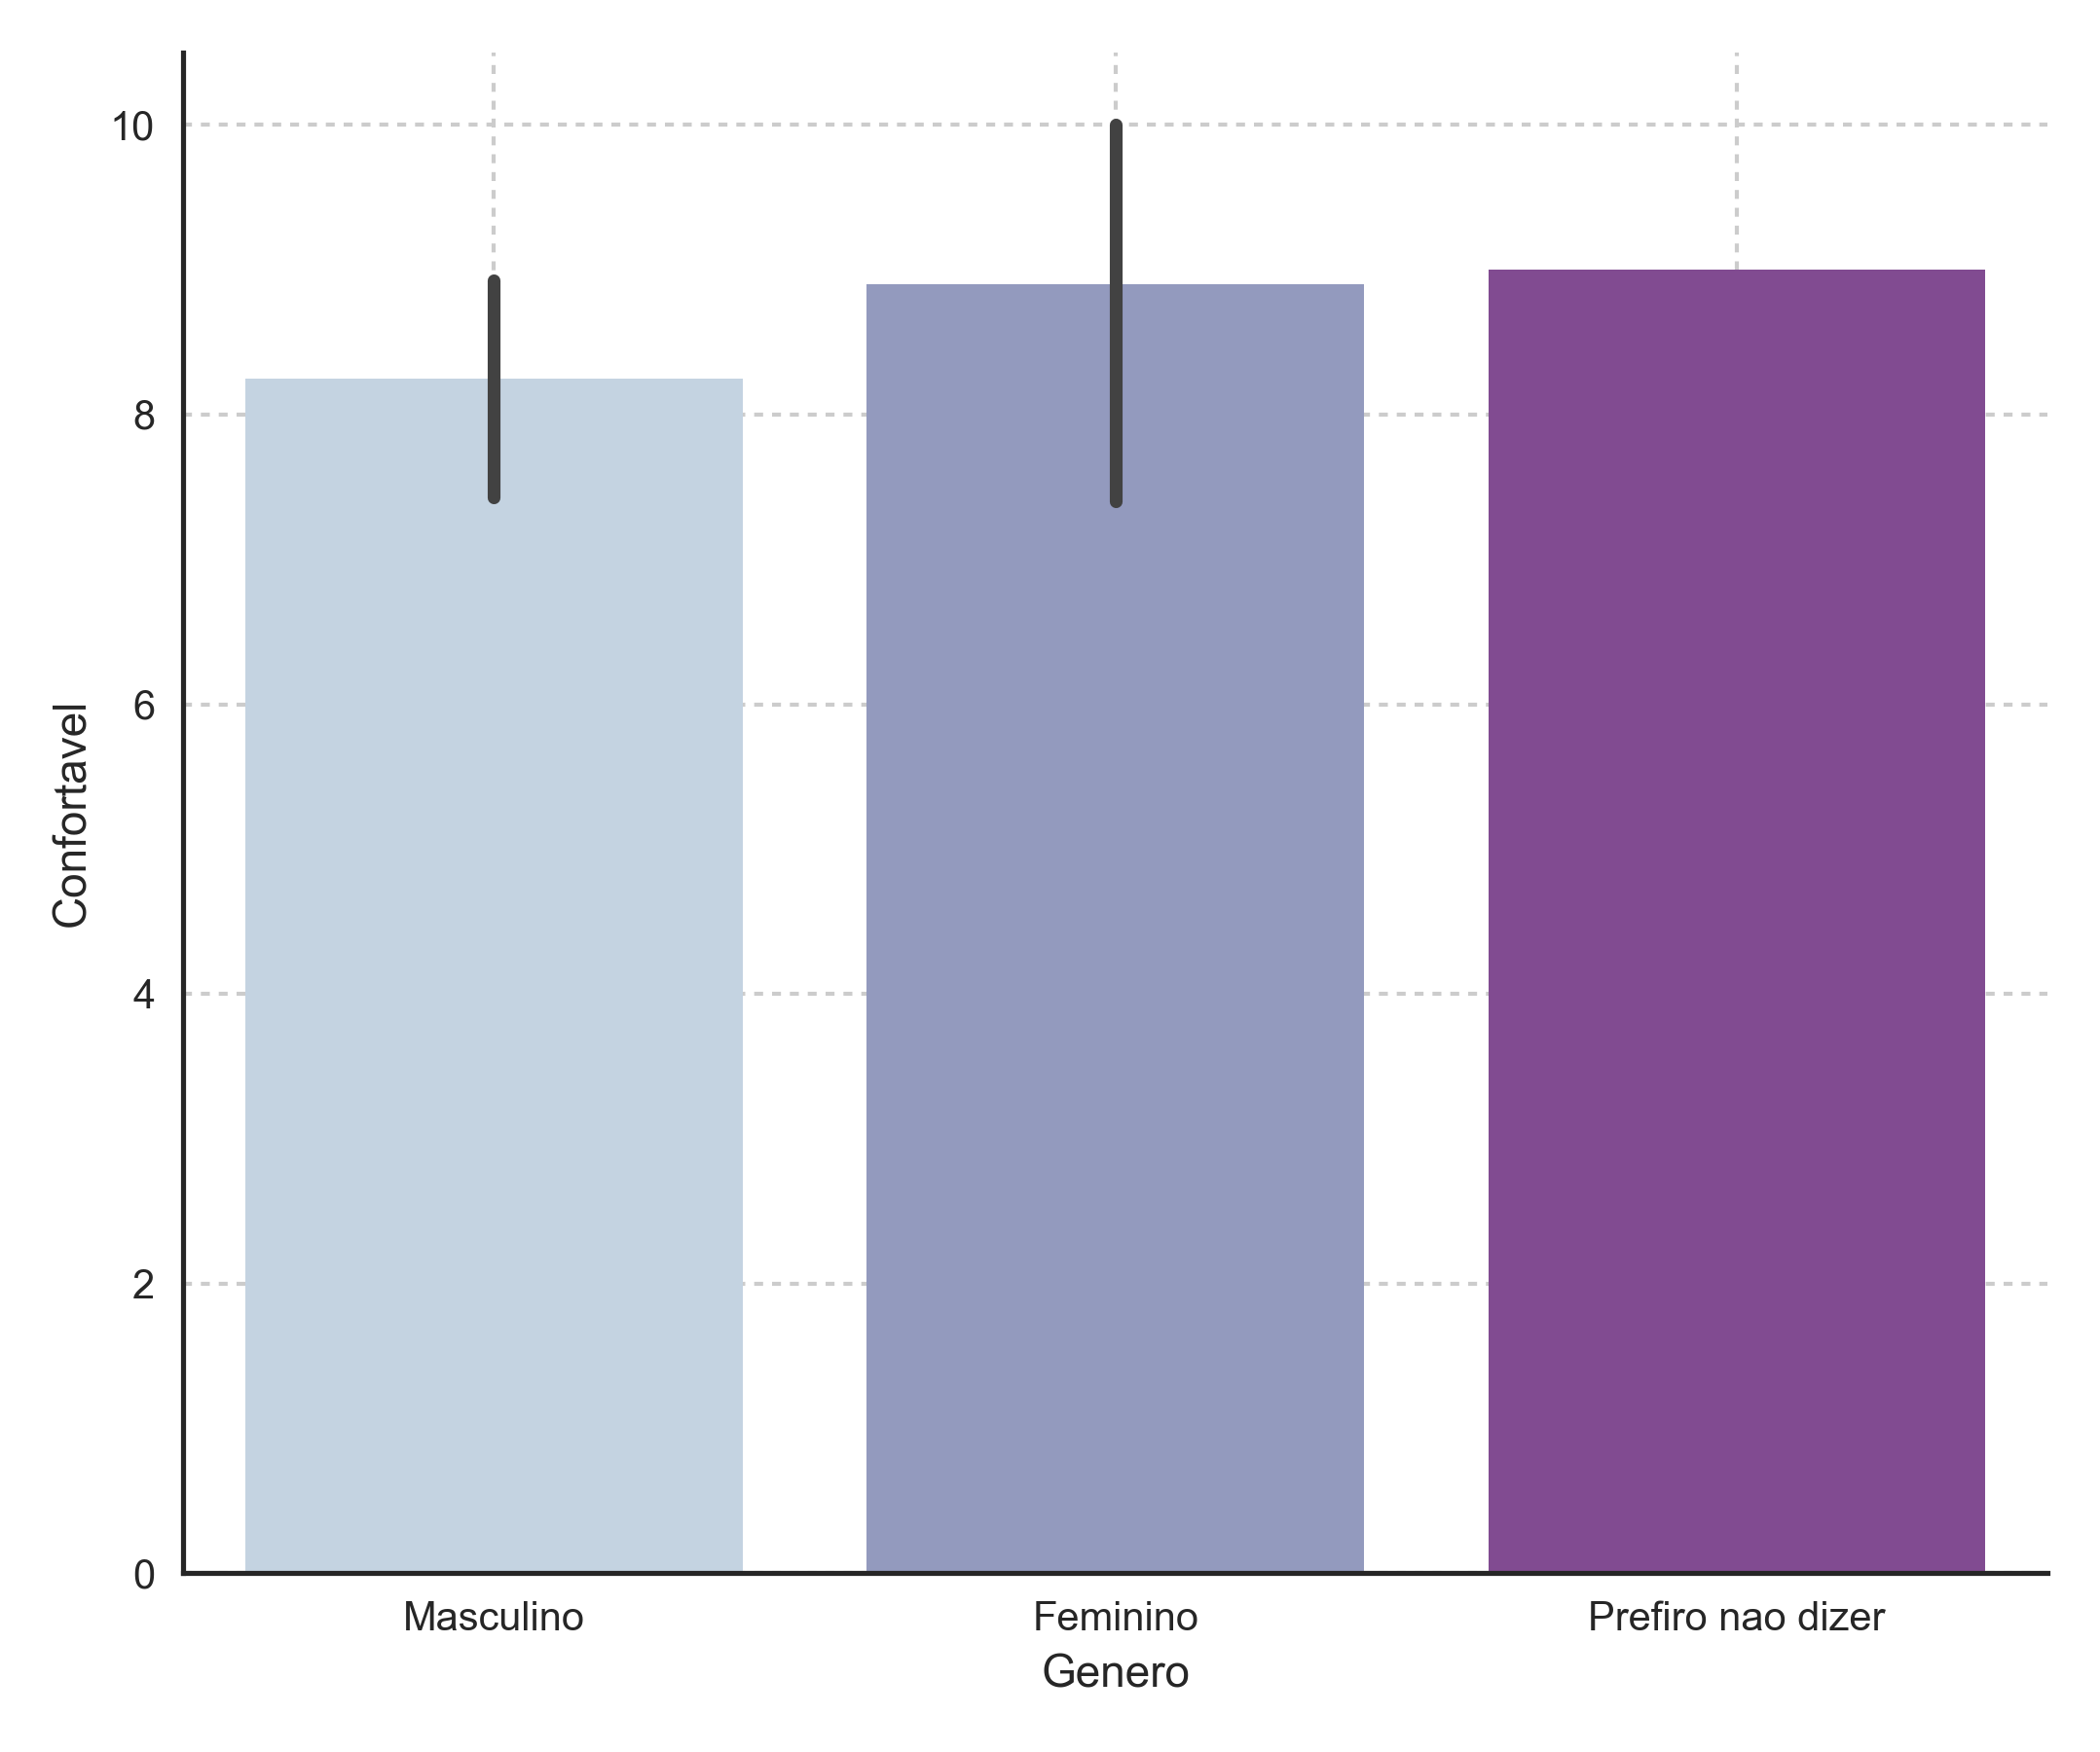
\includegraphics[width=\textwidth]{conforto_genero.png}
		\smallcaption{Fonte: O autor.}
		\label{fig:confortogenero}
	\end{minipage}
\end{figure}

Pode-se observar na figura~\ref{fig:confortogenero} que houve um equilíbrio entre os gêneros com relação ao conforto na aproximação do robô. Na média os homens ficaram 8.25 confortável na escala Likert, com o desvio padrão de 1.9933. As mulheres tiveram a média 8.9 e o desvio padrão em 2.0224. Isso ocorreu em grande parte devido a exibição das expressões faciais do robô. Os participantes do gênero feminino acolheram o robô como uma criança ou pessoa meiga se aproximando dela. Outra variável que é comparada é a idade dos partipantes com o nível de conforto, apresentado na figura~\ref{fig:confortoidade}.

\begin{figure}[ht!]
	\centering
	\begin{minipage}{0.65\textwidth}
		\caption{Conforto por idade.}
		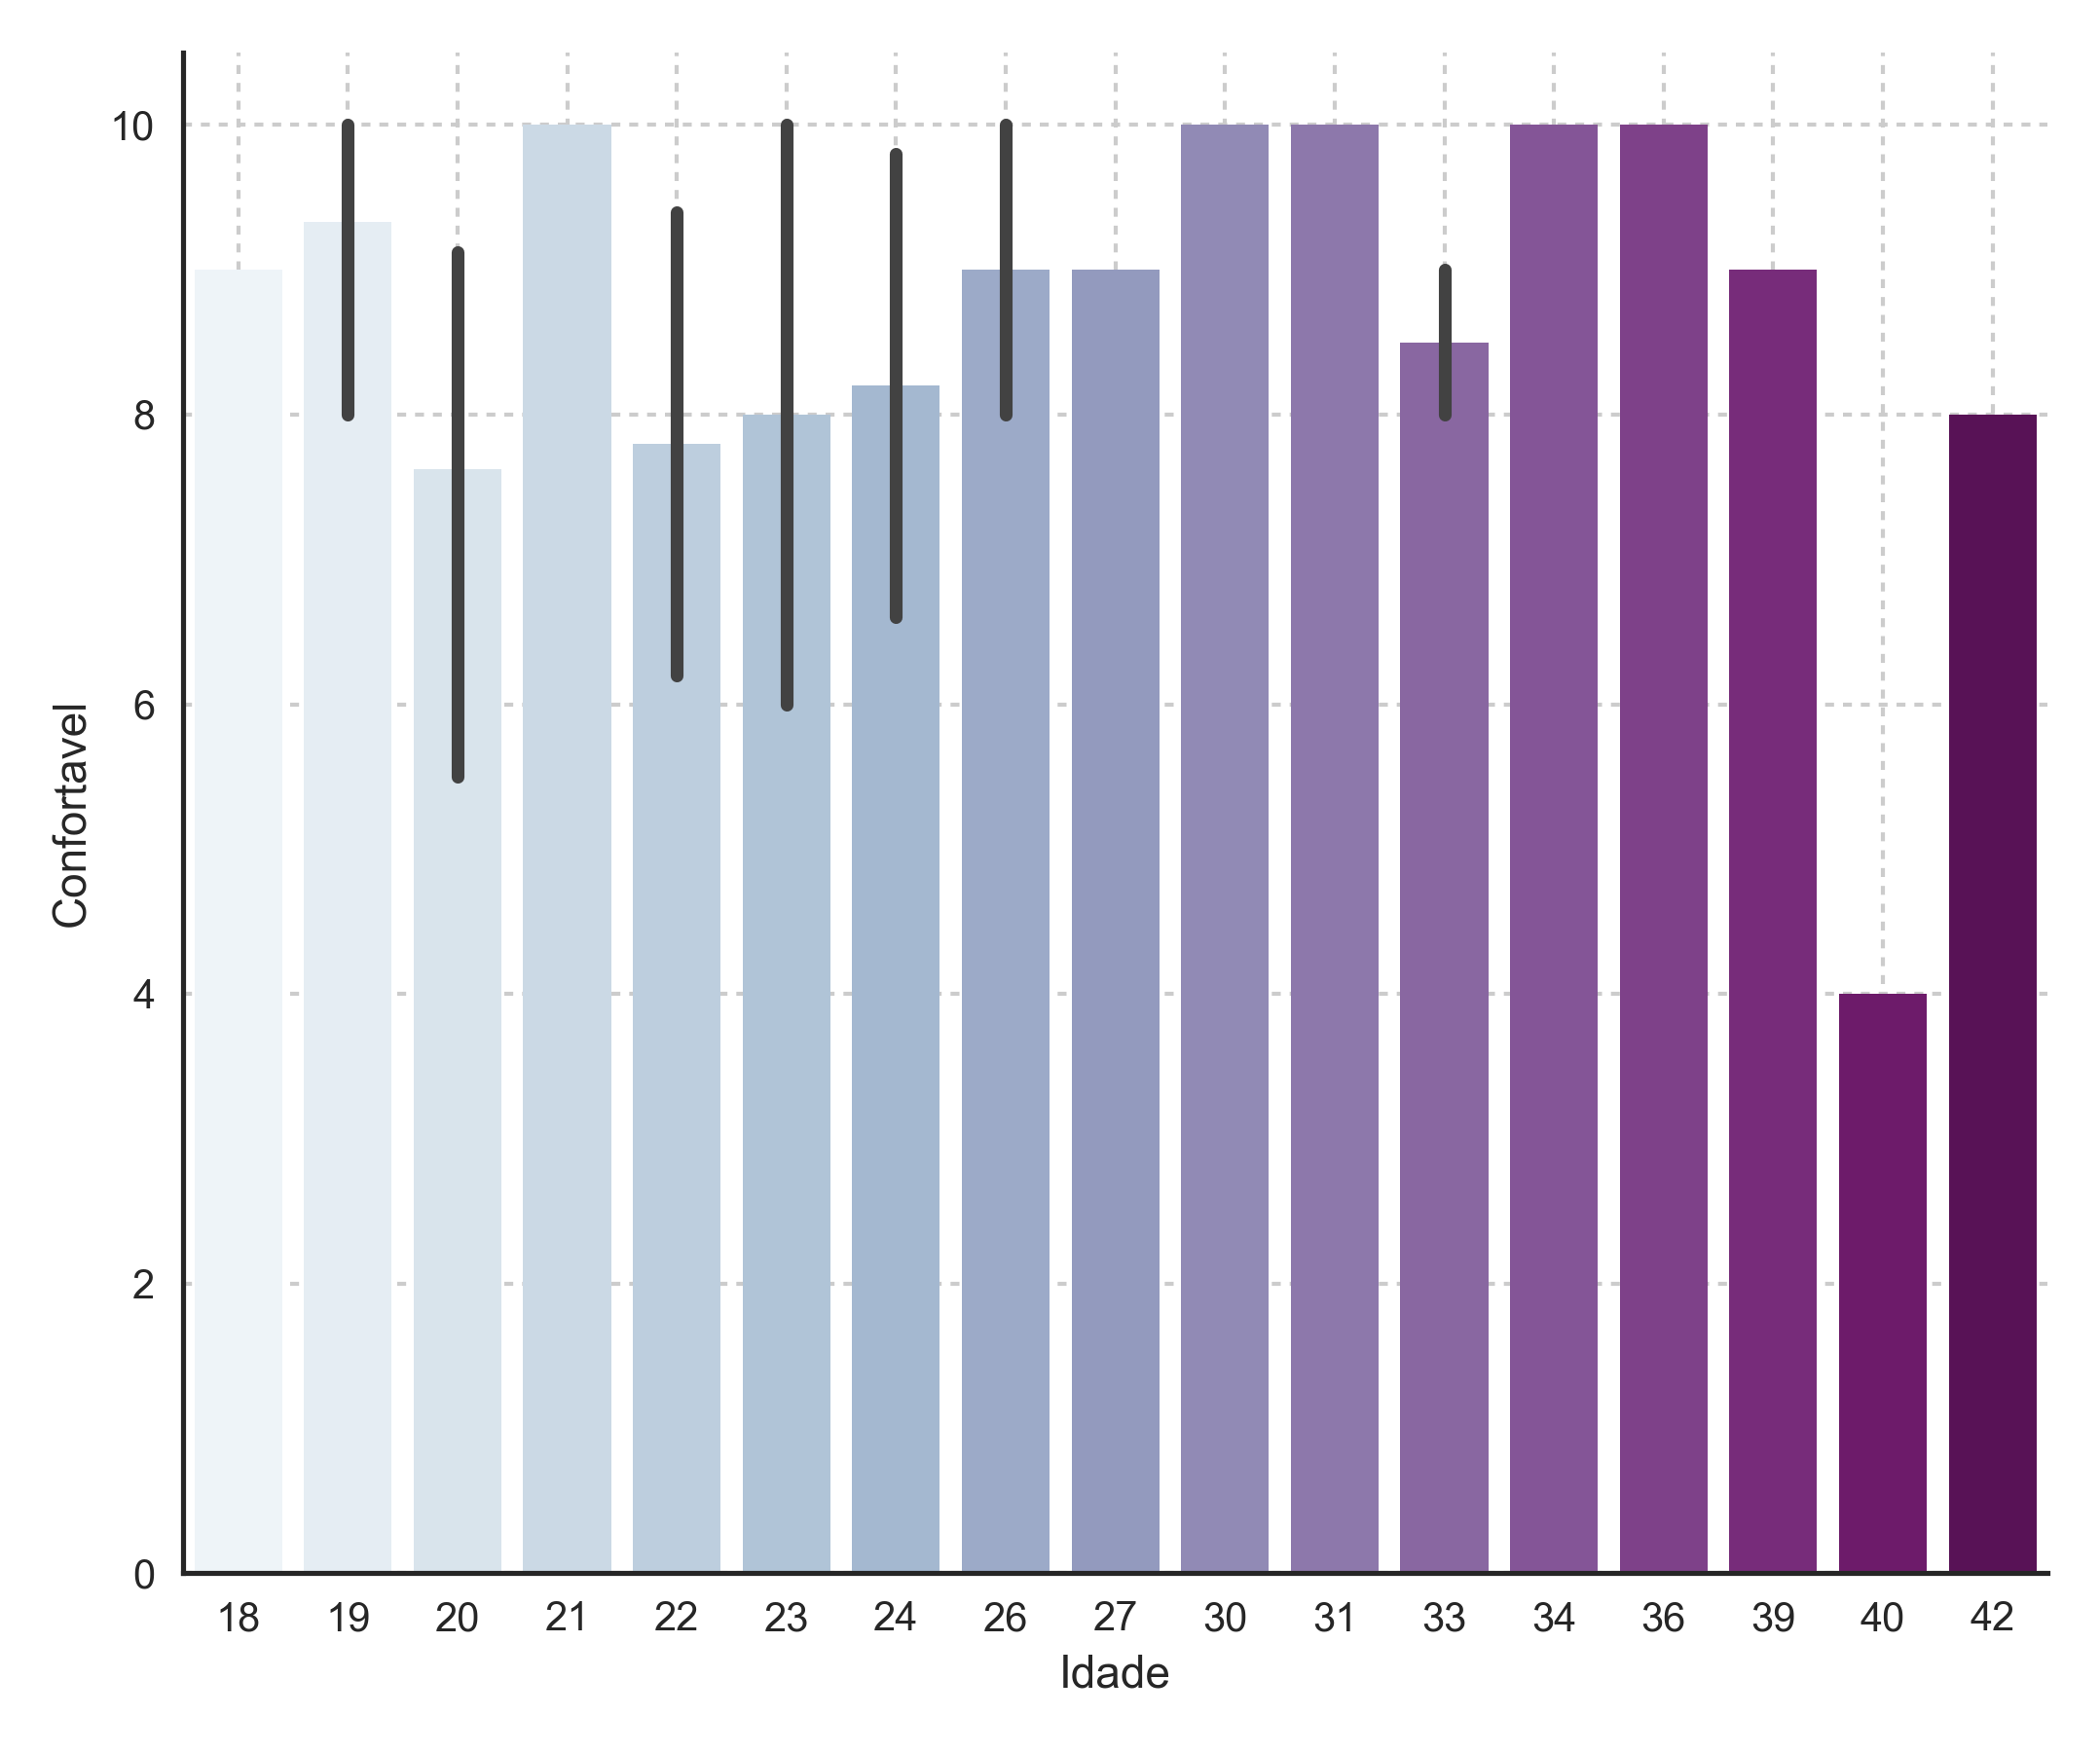
\includegraphics[width=\textwidth]{conforto_idade.png}
		\smallcaption{Fonte: O autor.}
		\label{fig:confortoidade}
	\end{minipage}
\end{figure}

Dois participantes apresentaram um nível de desconforto, mais elevado que os demais participantes, na aproximação do robô. Um participante apresentou a idade de 20 anos e outro de 40 anos. Foram os que ficaram mais desconfortáveis com o robô, como observado na figura~\ref{fig:confortoidade}. Os demais demonstraram-se confortavéis com o robô na aproximação.

Na figura~\ref{fig:confortoposicao} é apresentada a relação entre o conforto do participante e a posição dele durante a interação, sentado ou em pé.

\begin{figure}[ht!]
	\centering
	\begin{minipage}{0.65\textwidth}
		\caption{Conforto por posição de interação.}
		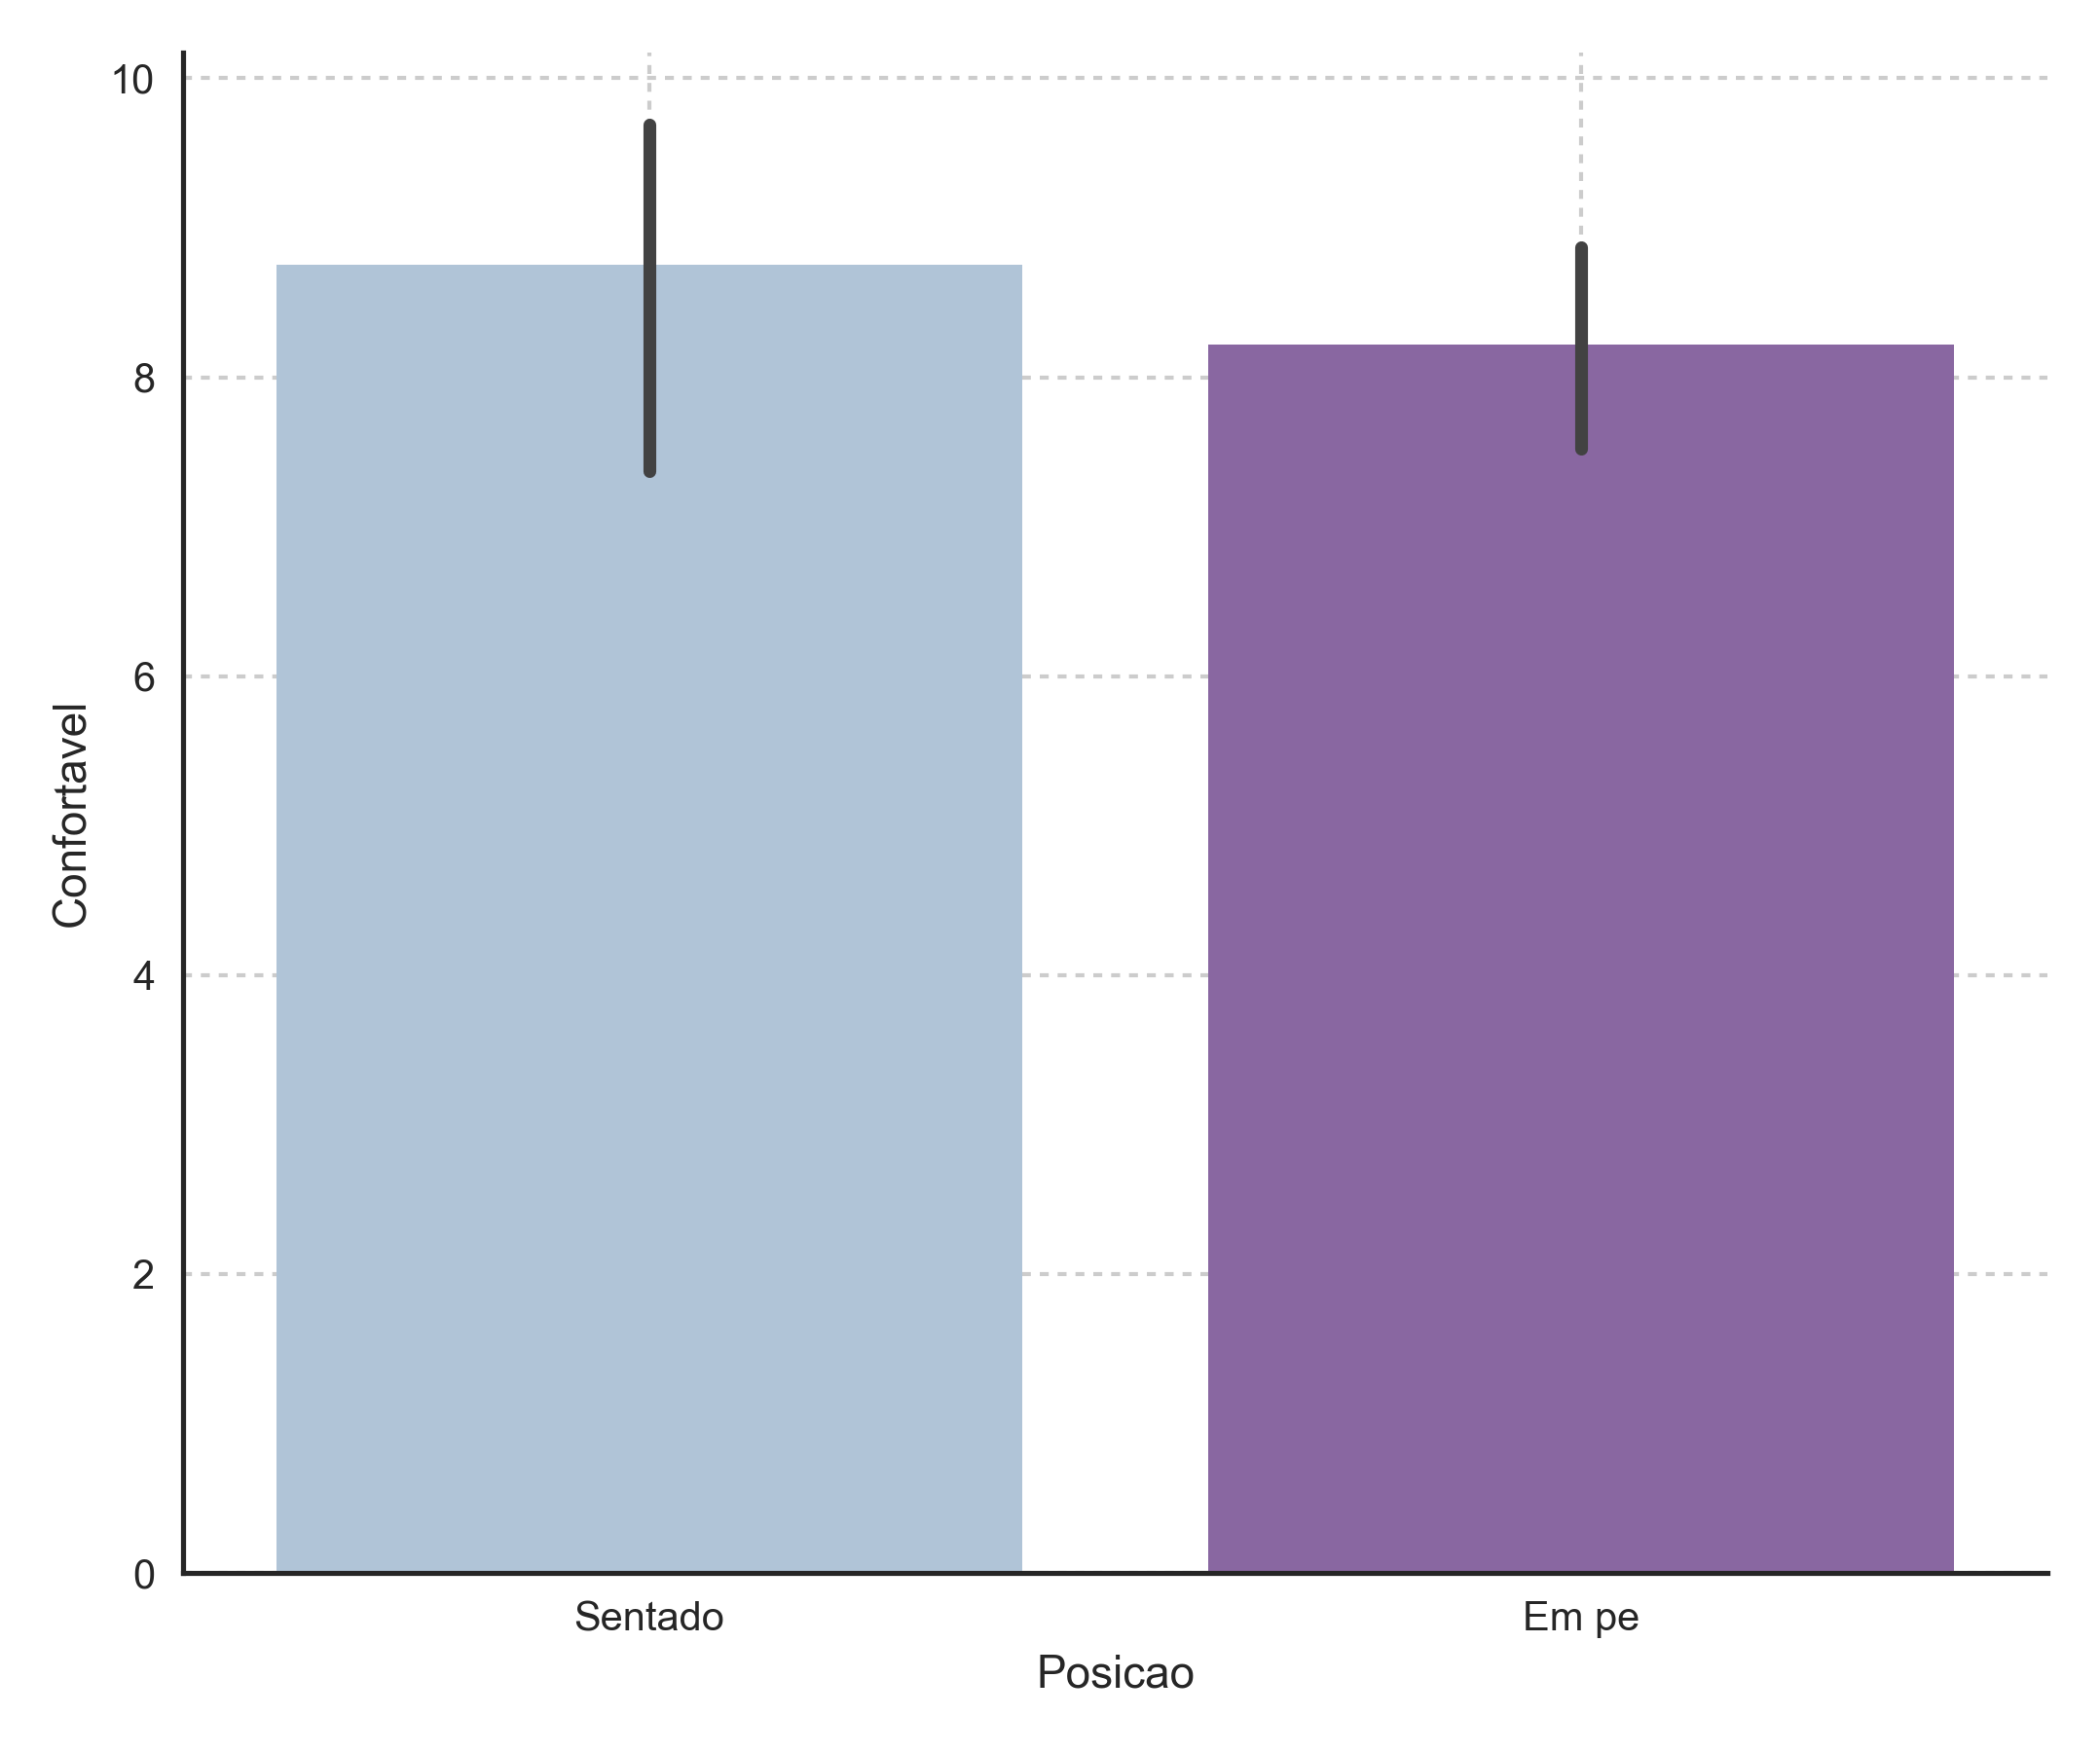
\includegraphics[width=\textwidth]{conforto_posicao.png}
		\smallcaption{Fonte: O autor.}
		\label{fig:confortoposicao}
	\end{minipage}
\end{figure}

É observado na figura~\ref{fig:confortoposicao} o oposto observado na competição da RoboCup@Home. Na competição, as pessoas sentadas sentiram-se com maior desconforto. Nos testes, as pessoas que estavam sentadas durante a interação com o robô sentiram-se mais confortavéis do que as pessoas que estavam em pé. Na média as pessoas em pé apresentaram um grau de conforto igual a 8.2174 e desvio padrão de 1.6407. Já as pessoas sentadas mativeral uma média de 8.75 de grau de conforto, com desvio padrão 2.3848. Esse fenômeno ocorreu, pois o robô tocou no braço e barriga de alguns participantes que estavam em pé quando esticou o manipulador para chamar a atenção deles. O fenômeno do toque é um ponto de atenção que deve ser tratado em uma nova iteração do ciclo de desenvolvimento do projeto, como uma futura evolução no controle do manipulador. Por último, é apresentado na figura~\ref{fig:confortosociavel} o nível de conforto dos participantes, dado a sua declaração de sociável ou não.

\begin{figure}[ht!]
	\centering
	\begin{minipage}{0.65\textwidth}
		\caption{Conforto por declaração de sociável.}
		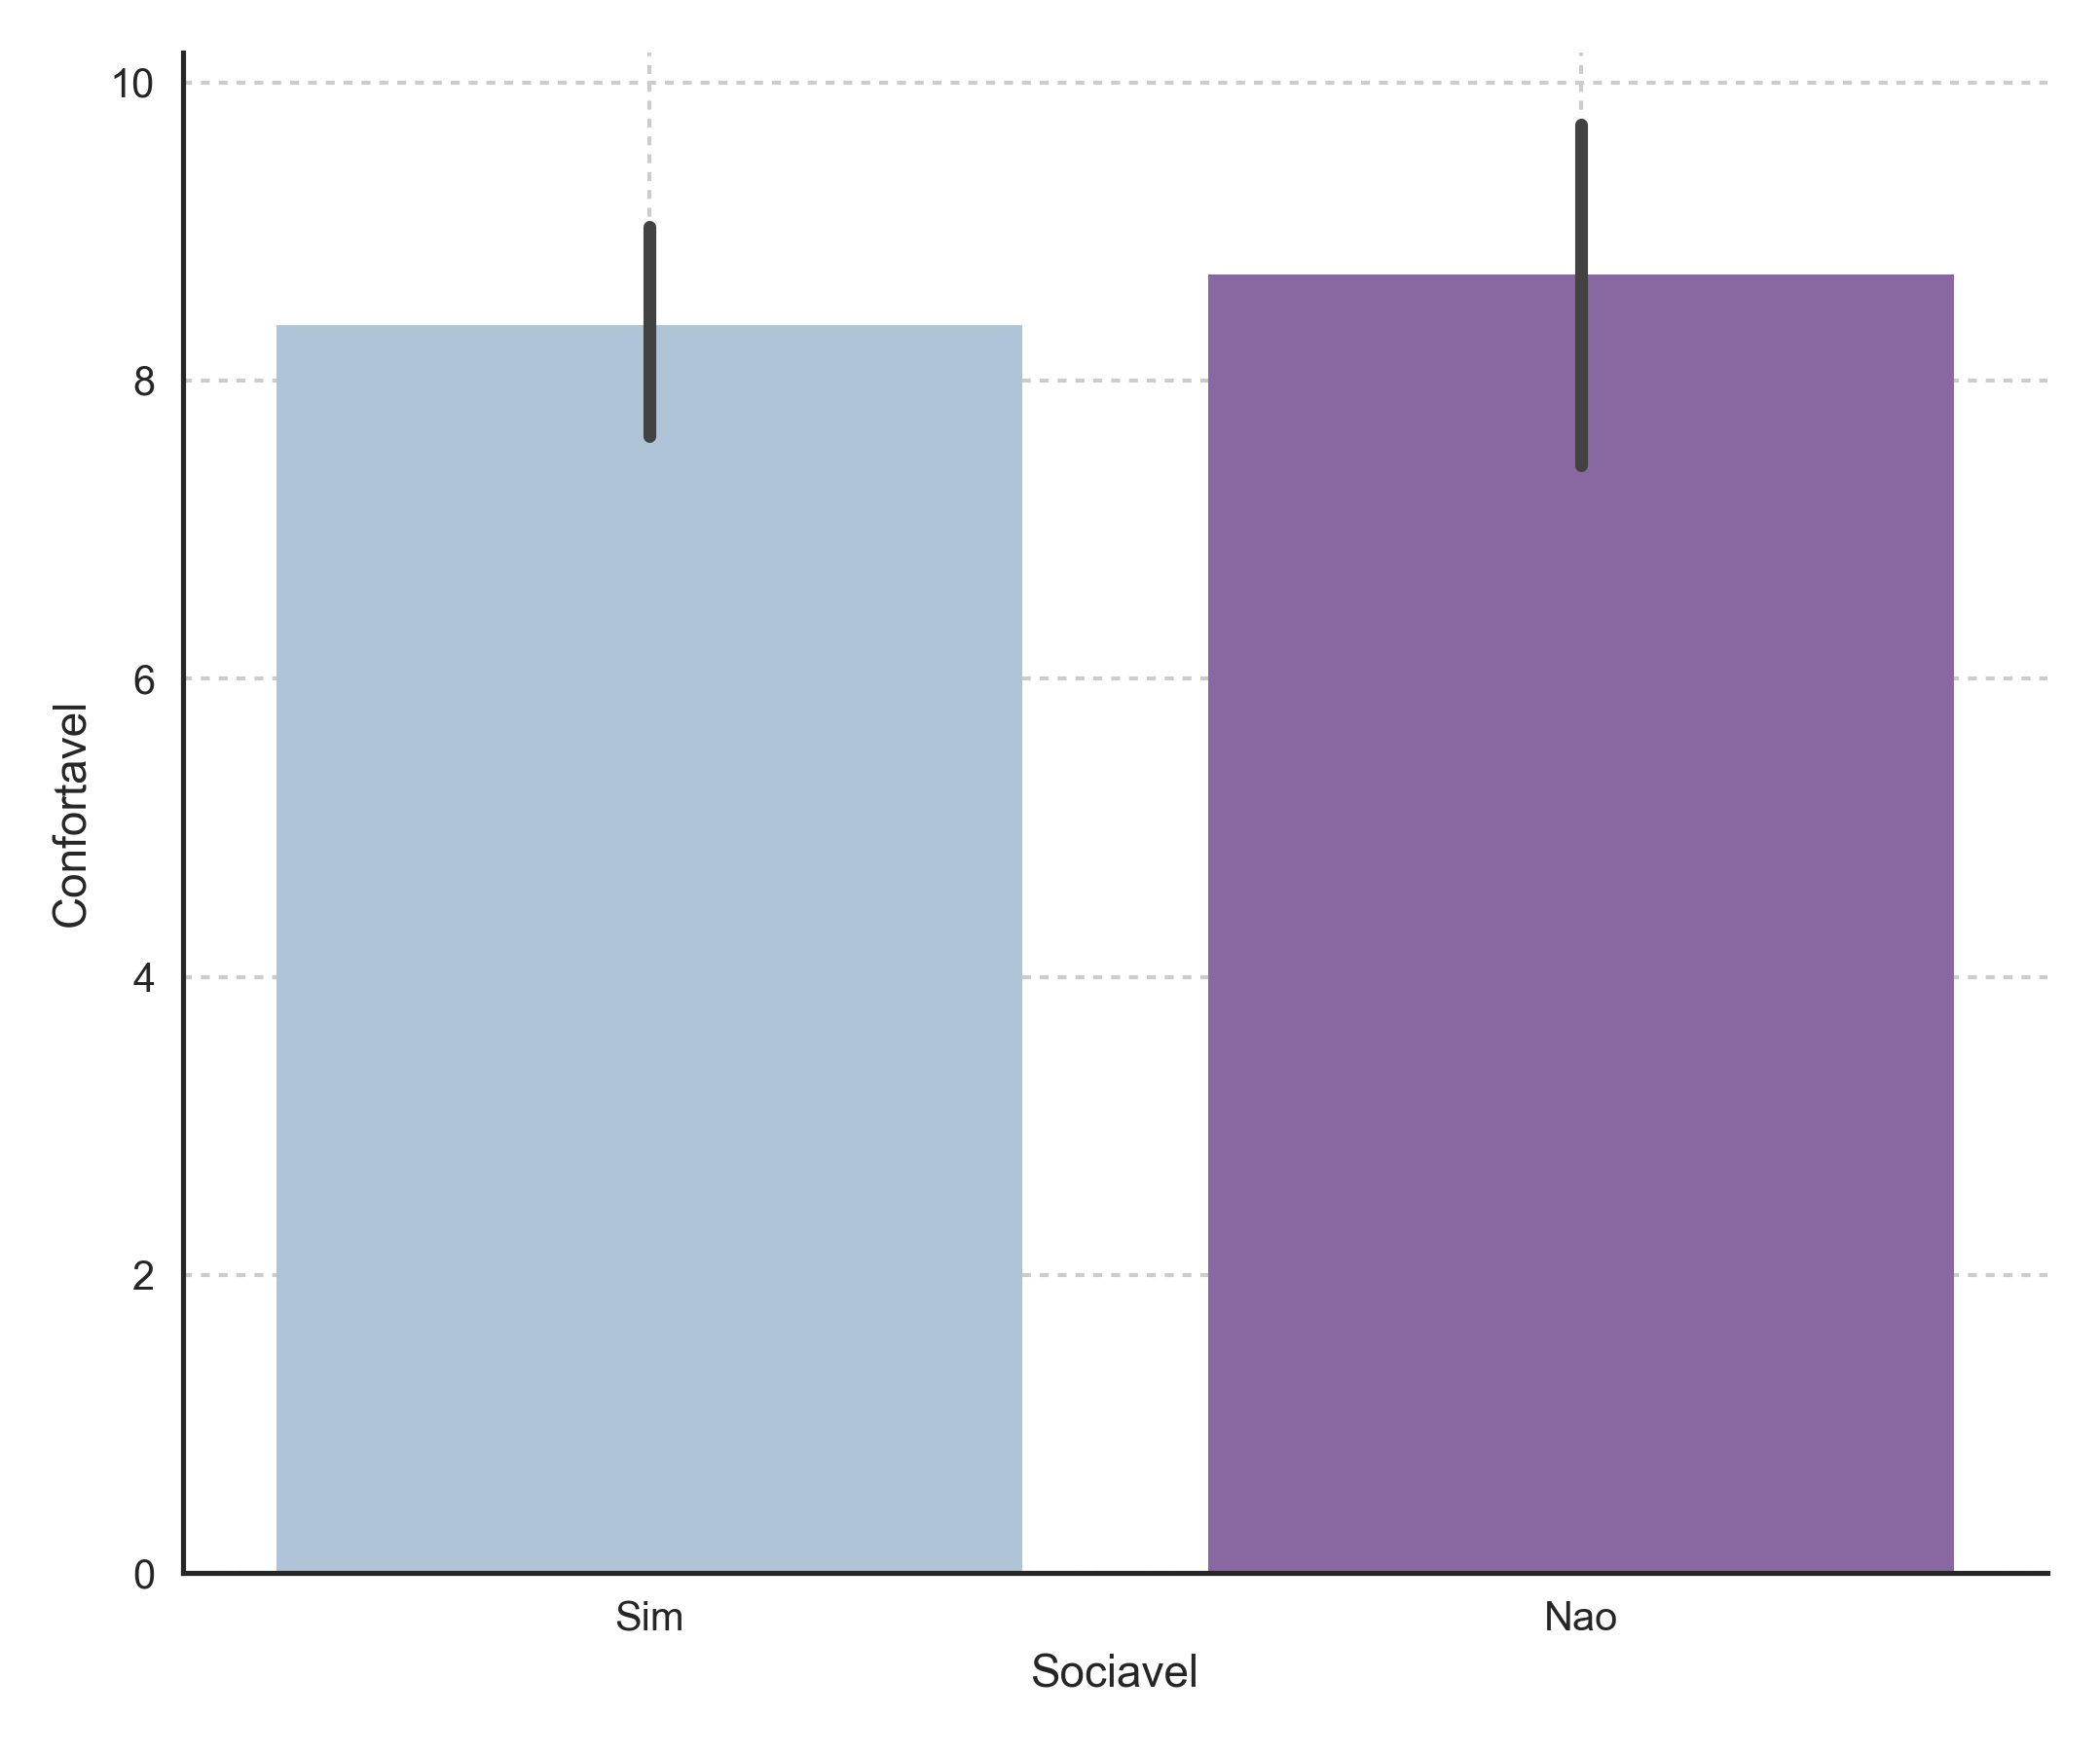
\includegraphics[width=\textwidth]{conforto_sociavel.png}
		\smallcaption{Fonte: O autor.}
		\label{fig:confortosociavel}
	\end{minipage}
\end{figure}

Nessa análise feita através da figura~\ref{fig:confortosociavel}, as pessoas declaradas como não sociáveis, foram as pessoas que mais se sentiram confortáveis durante toda a aproximação do robô. Na média uma pessoa sociável apresentou um grau de conforto de 8.375, com desvio padrão de 2.0729. Já a pessoa não sociável apresentou 8.7143 na média, com desvio padrão de 1.5779. É um ponto interessante, pois se observar, as pessoas sociáveis deveriam estar mais confortável e abertas a novas experiências.

Algumas situações durante o cenário de interação causaram medo, como por exemplo, o manipulador tocado o participante. E na mesma situação, o usuário ficou confortável ao ver a expressão facial amigável do robô, esboçando um sorriso. Assim, a mesma análise para o conforto do usuário, foi realizada para a declaração de medo. Na escala da pergunta sobre medo do robô, o menor valor corresponde a totalmente com medo (valor 0 da escala) e o maior corresponde a totalmente sem medo (valor 10 da escala). A figura~\ref{fig:medogenero} apresenta a relação entre o medo e o gênero do participante.

\begin{figure}[ht!]
	\centering
	\begin{minipage}{0.65\textwidth}
		\caption{Medo por gênero.}
		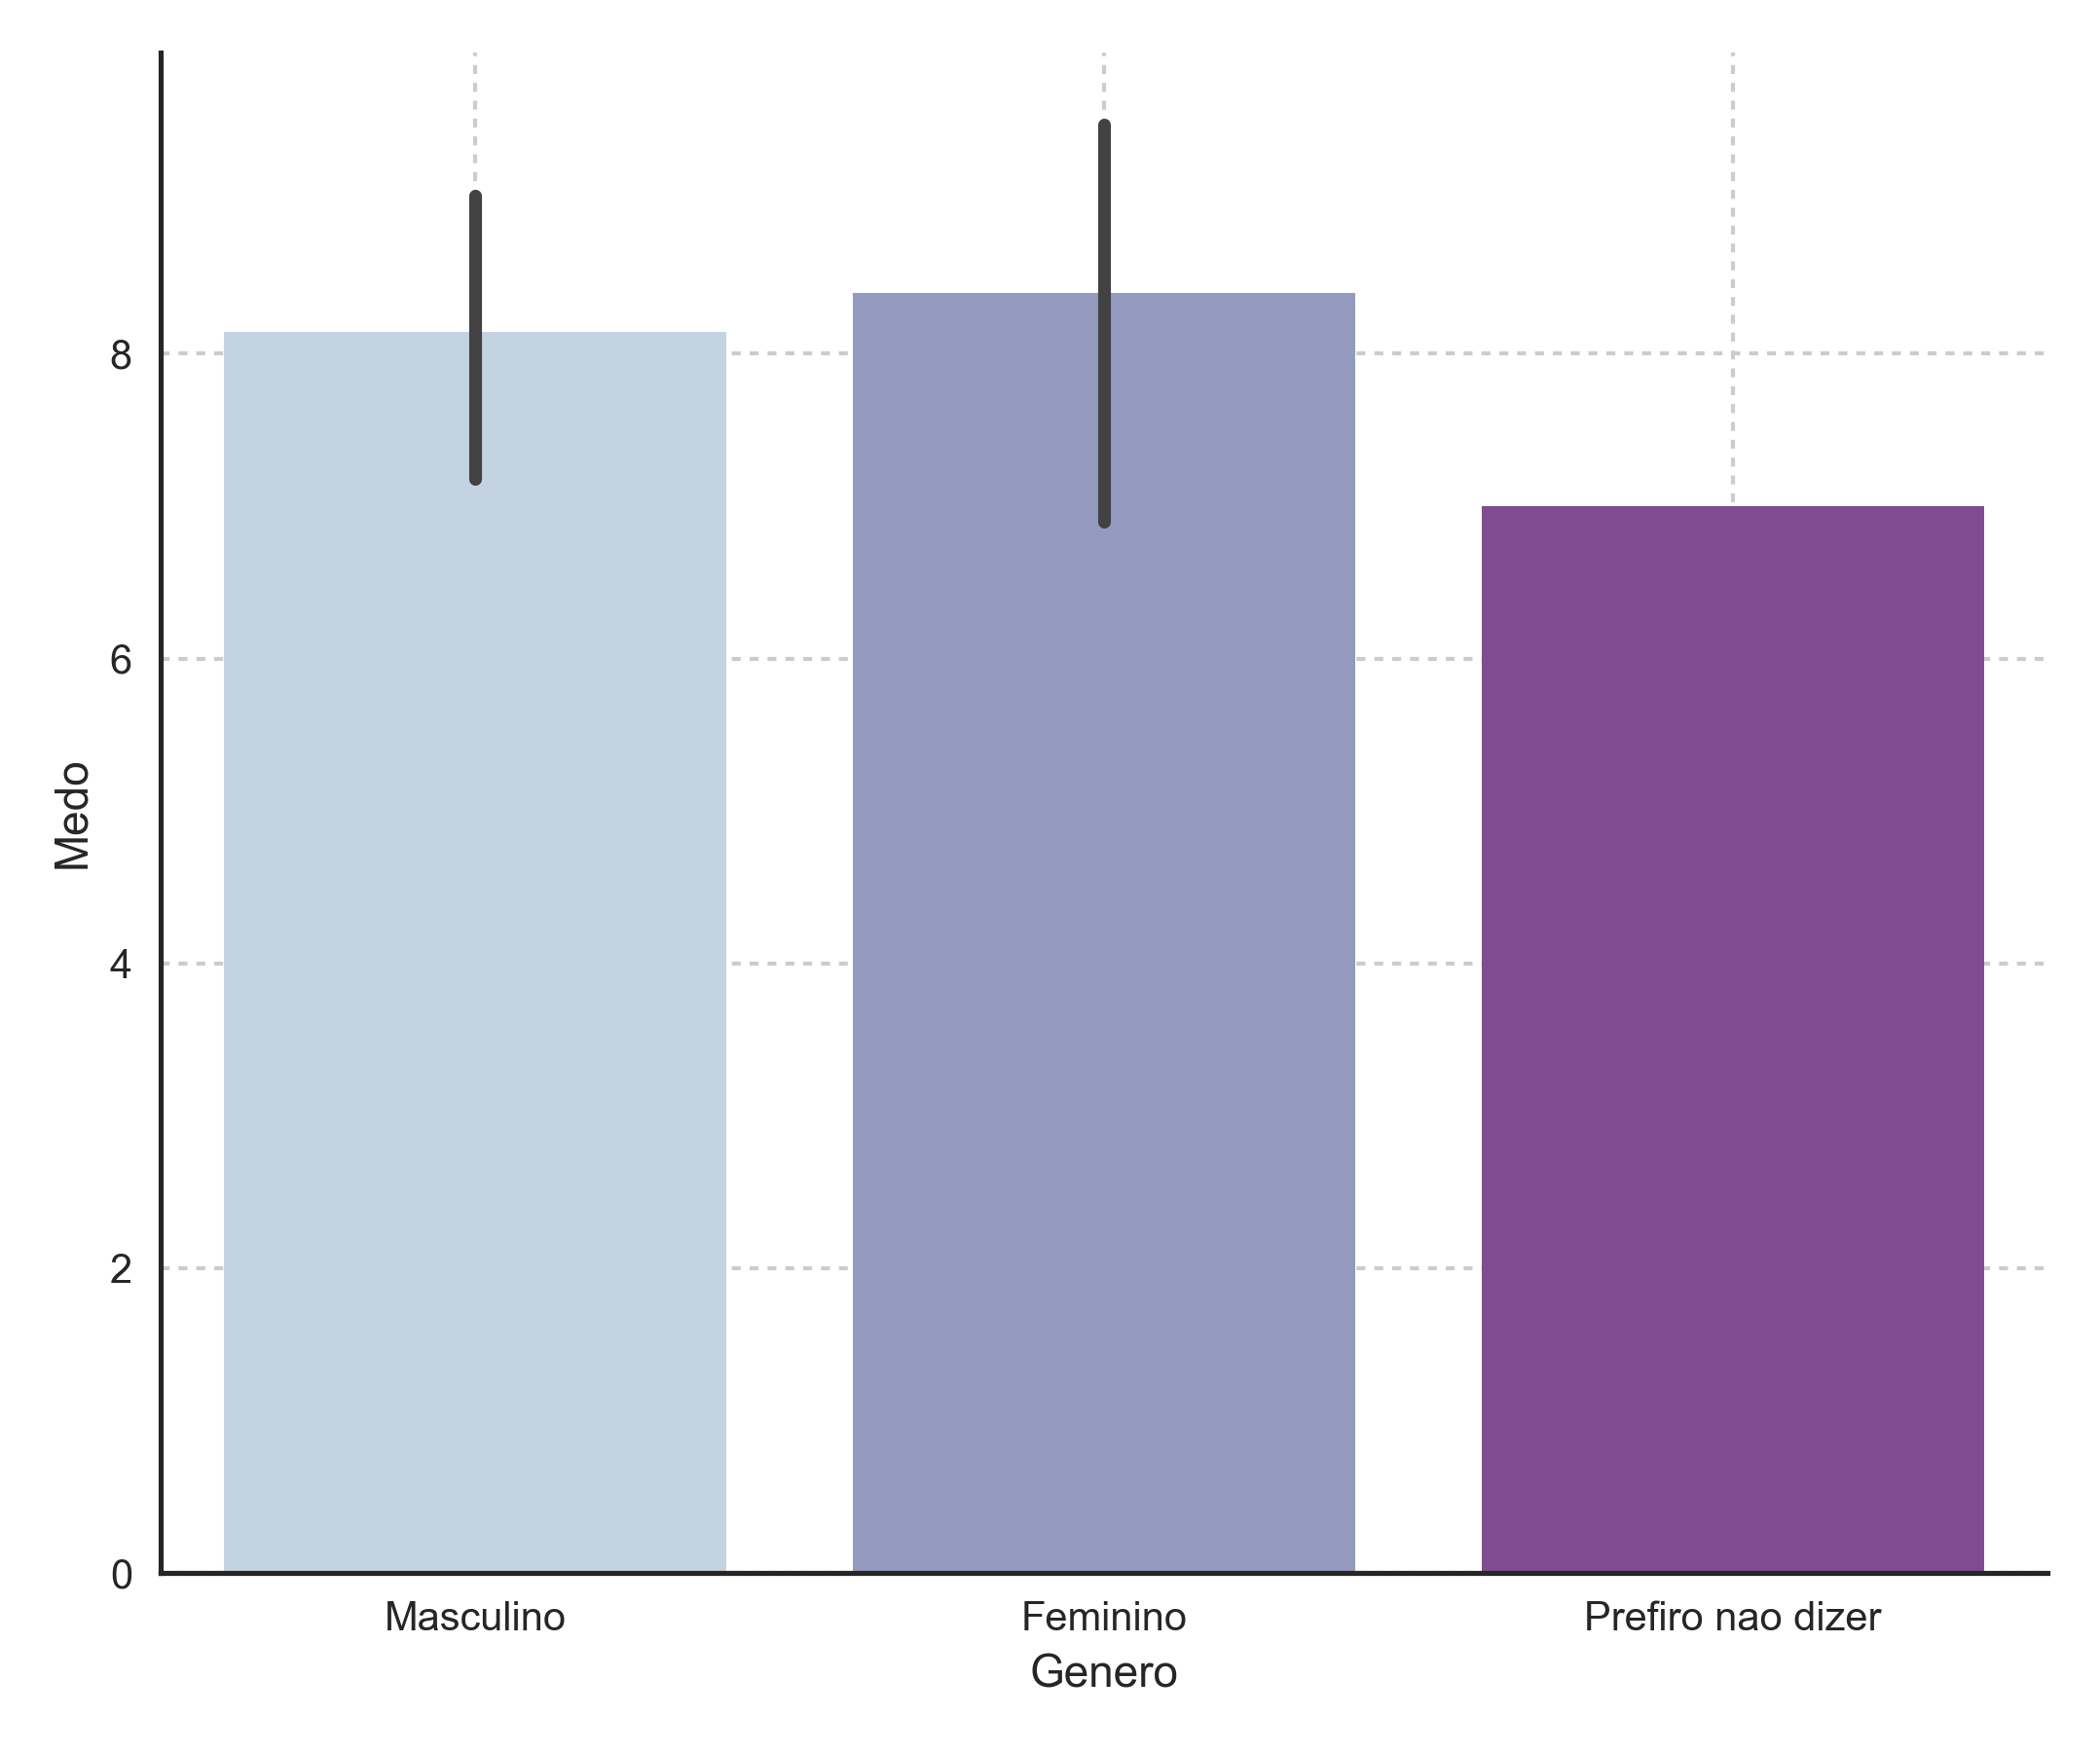
\includegraphics[width=\textwidth]{medo_genero.png}
		\smallcaption{Fonte: O autor.}
		\label{fig:medogenero}
	\end{minipage}
\end{figure}

Para a relação de medo e gênero, o que observa-se na figura~\ref{fig:medogenero} é que o gênero feminino sentiu menos medo. Porém, a diferença não foi tão grande assim. Na média as mulheres tiveram 8.4 graus, com desvio padrão de 2.1071. Enquanto isso, os homens ficaram com a média de 8.1429, desvio padrão de 2.6010. Era esperado este resultado, devido as observações sobre o conforto do usuário, apesar dessa relação nem sempre ser diretamente proporcional. Na sequência é feita a análise com base na relação medo e idade, demonstrada na figura~\ref{fig:medoidade}.

\begin{figure}[ht!]
	\centering
	\begin{minipage}{0.65\textwidth}
		\caption{Medo por idade.}
		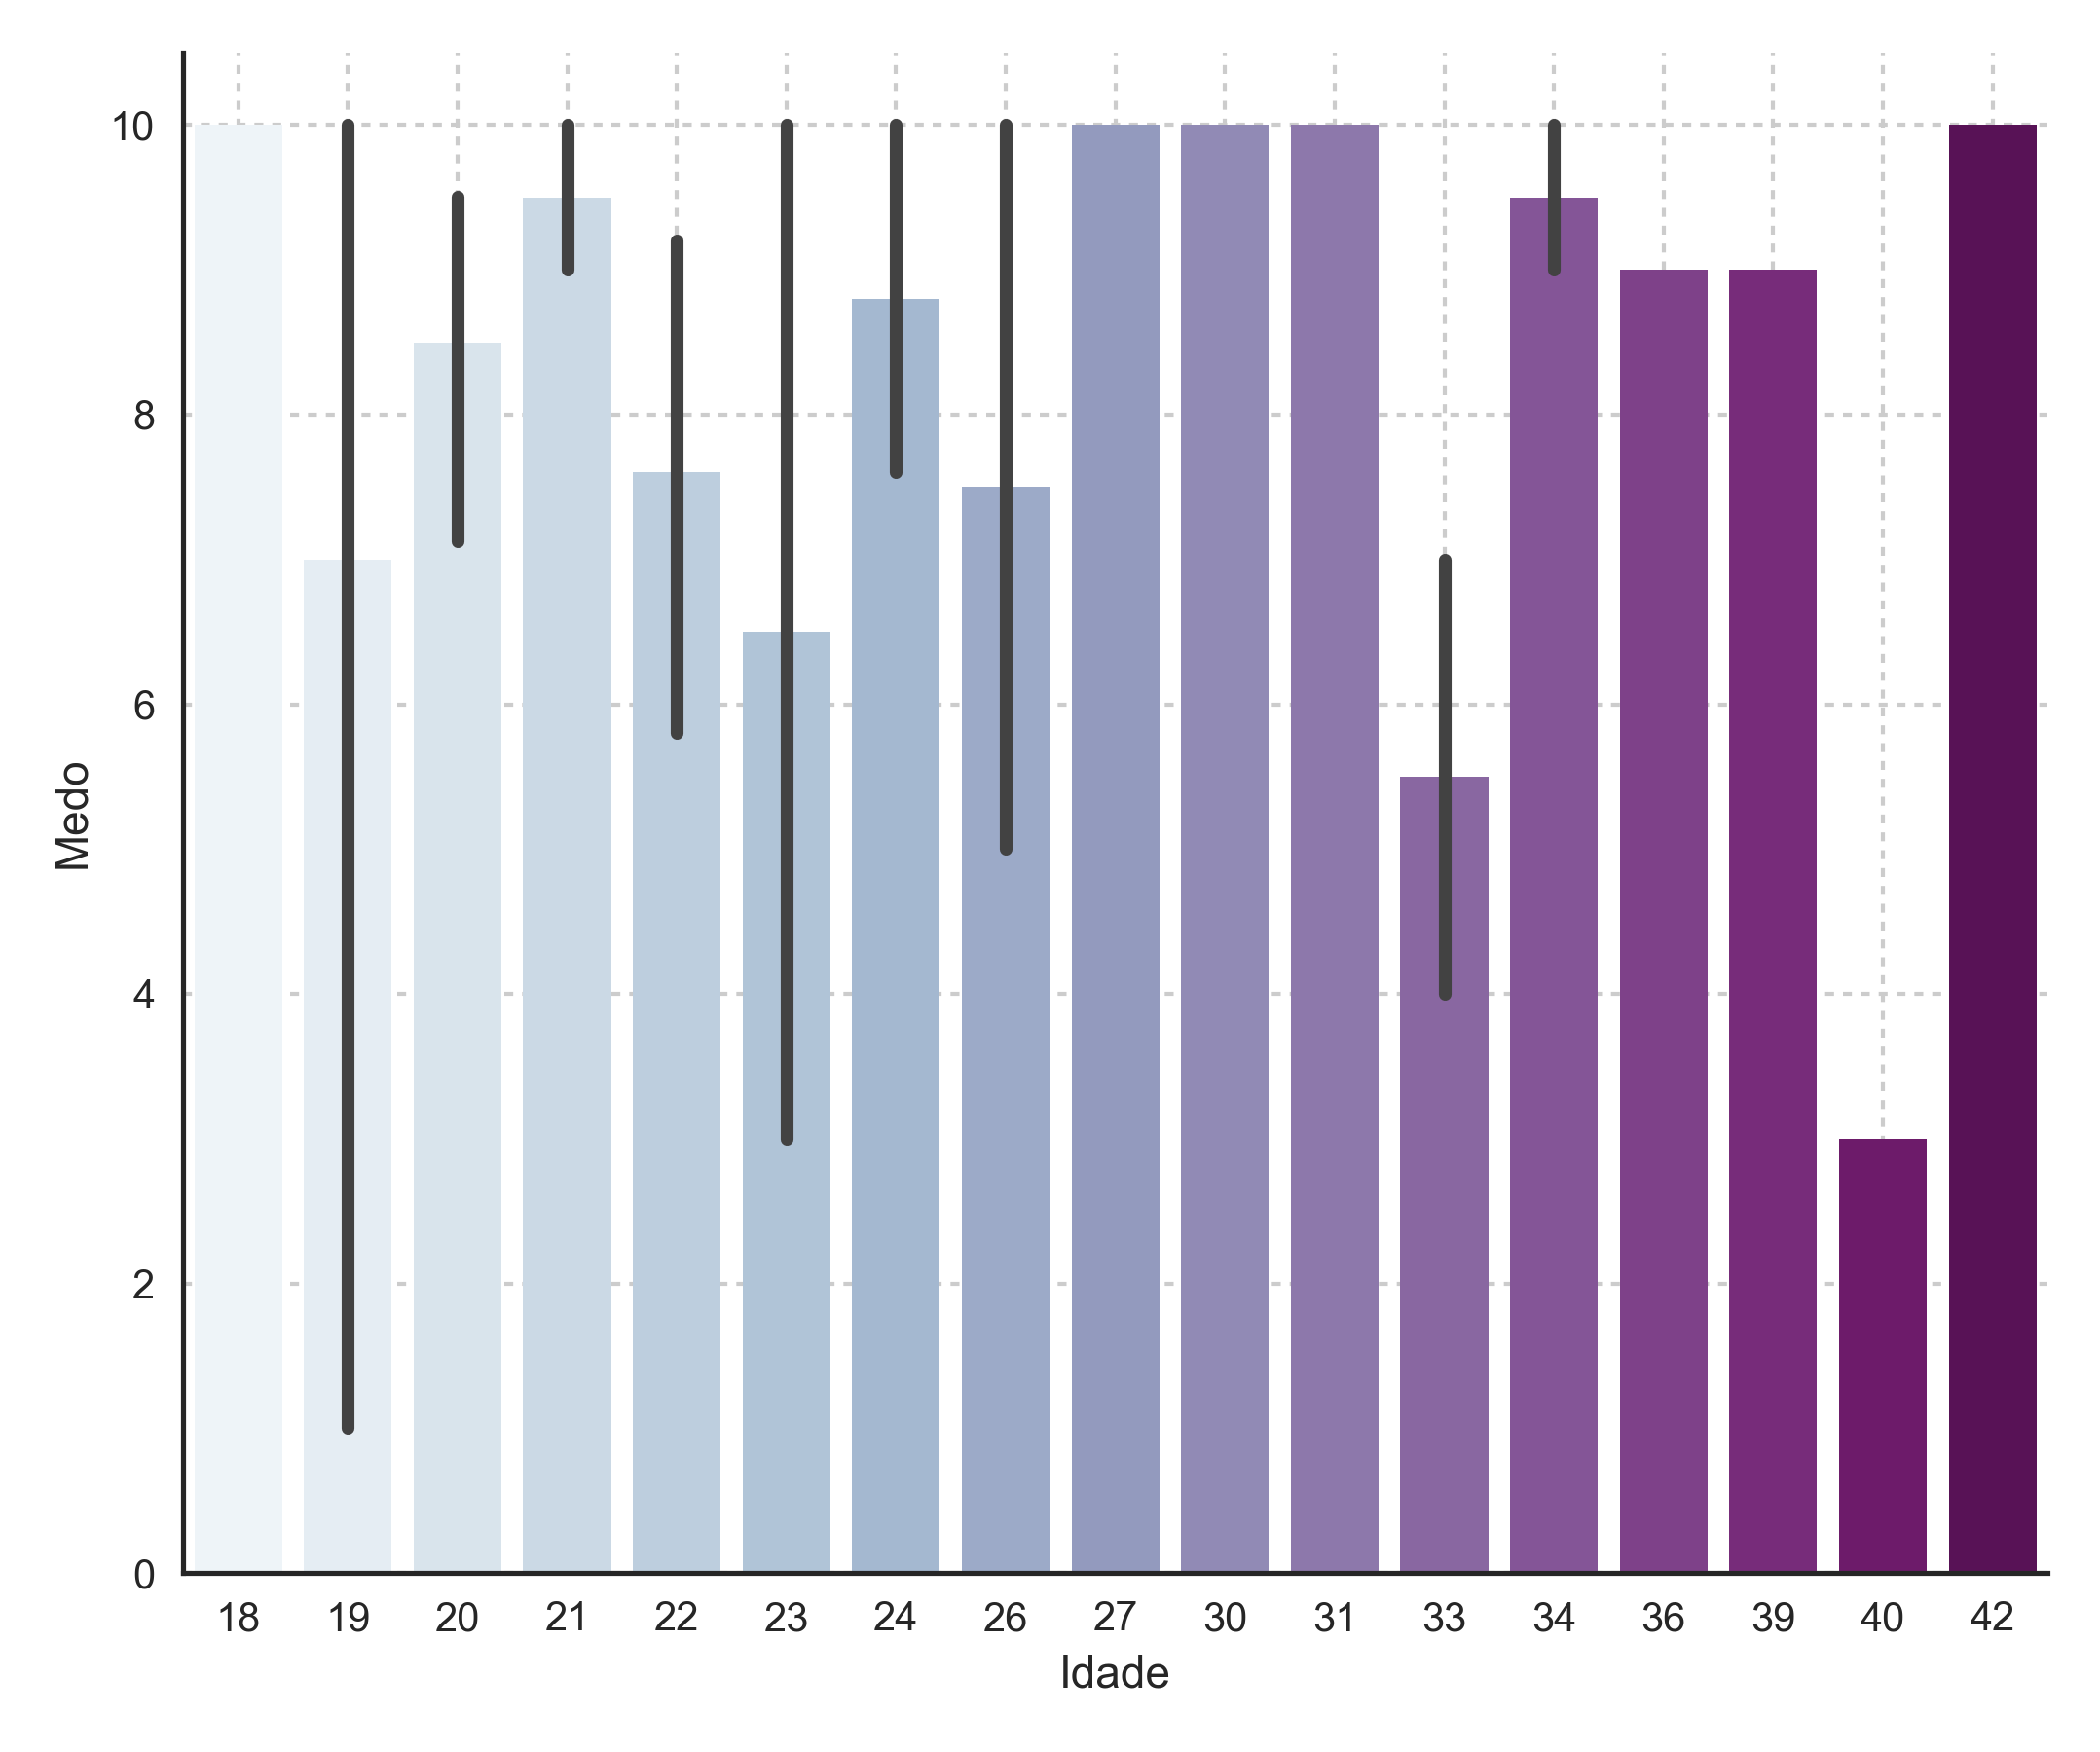
\includegraphics[width=\textwidth]{medo_idade.png}
		\smallcaption{Fonte: O autor.}
		\label{fig:medoidade}
	\end{minipage}
\end{figure}

Um participante na faixa etária de 40 anos, apresentou o maior índice de medo, conforme figura~\ref{fig:medoidade}. Os participantes com 19 anos também apresentam um índice baixo, que indica medo do participante. Isso ocorreu, pois com o comportamento invasivo do robô ao aproximar, a garra deixou o participante assustado. Outro ponto levantado foi que o robô ao se movimentar faz muito barulho, devido ao novo conjunto de rodas omnidirecionais.

A figura~\ref{fig:medoposicao} compara a relação do medo declarado do usuário contra a posição dele durante a navegação do robô.

\begin{figure}[ht!]
	\centering
	\begin{minipage}{0.65\textwidth}
		\caption{Medo por posição de interação.}
		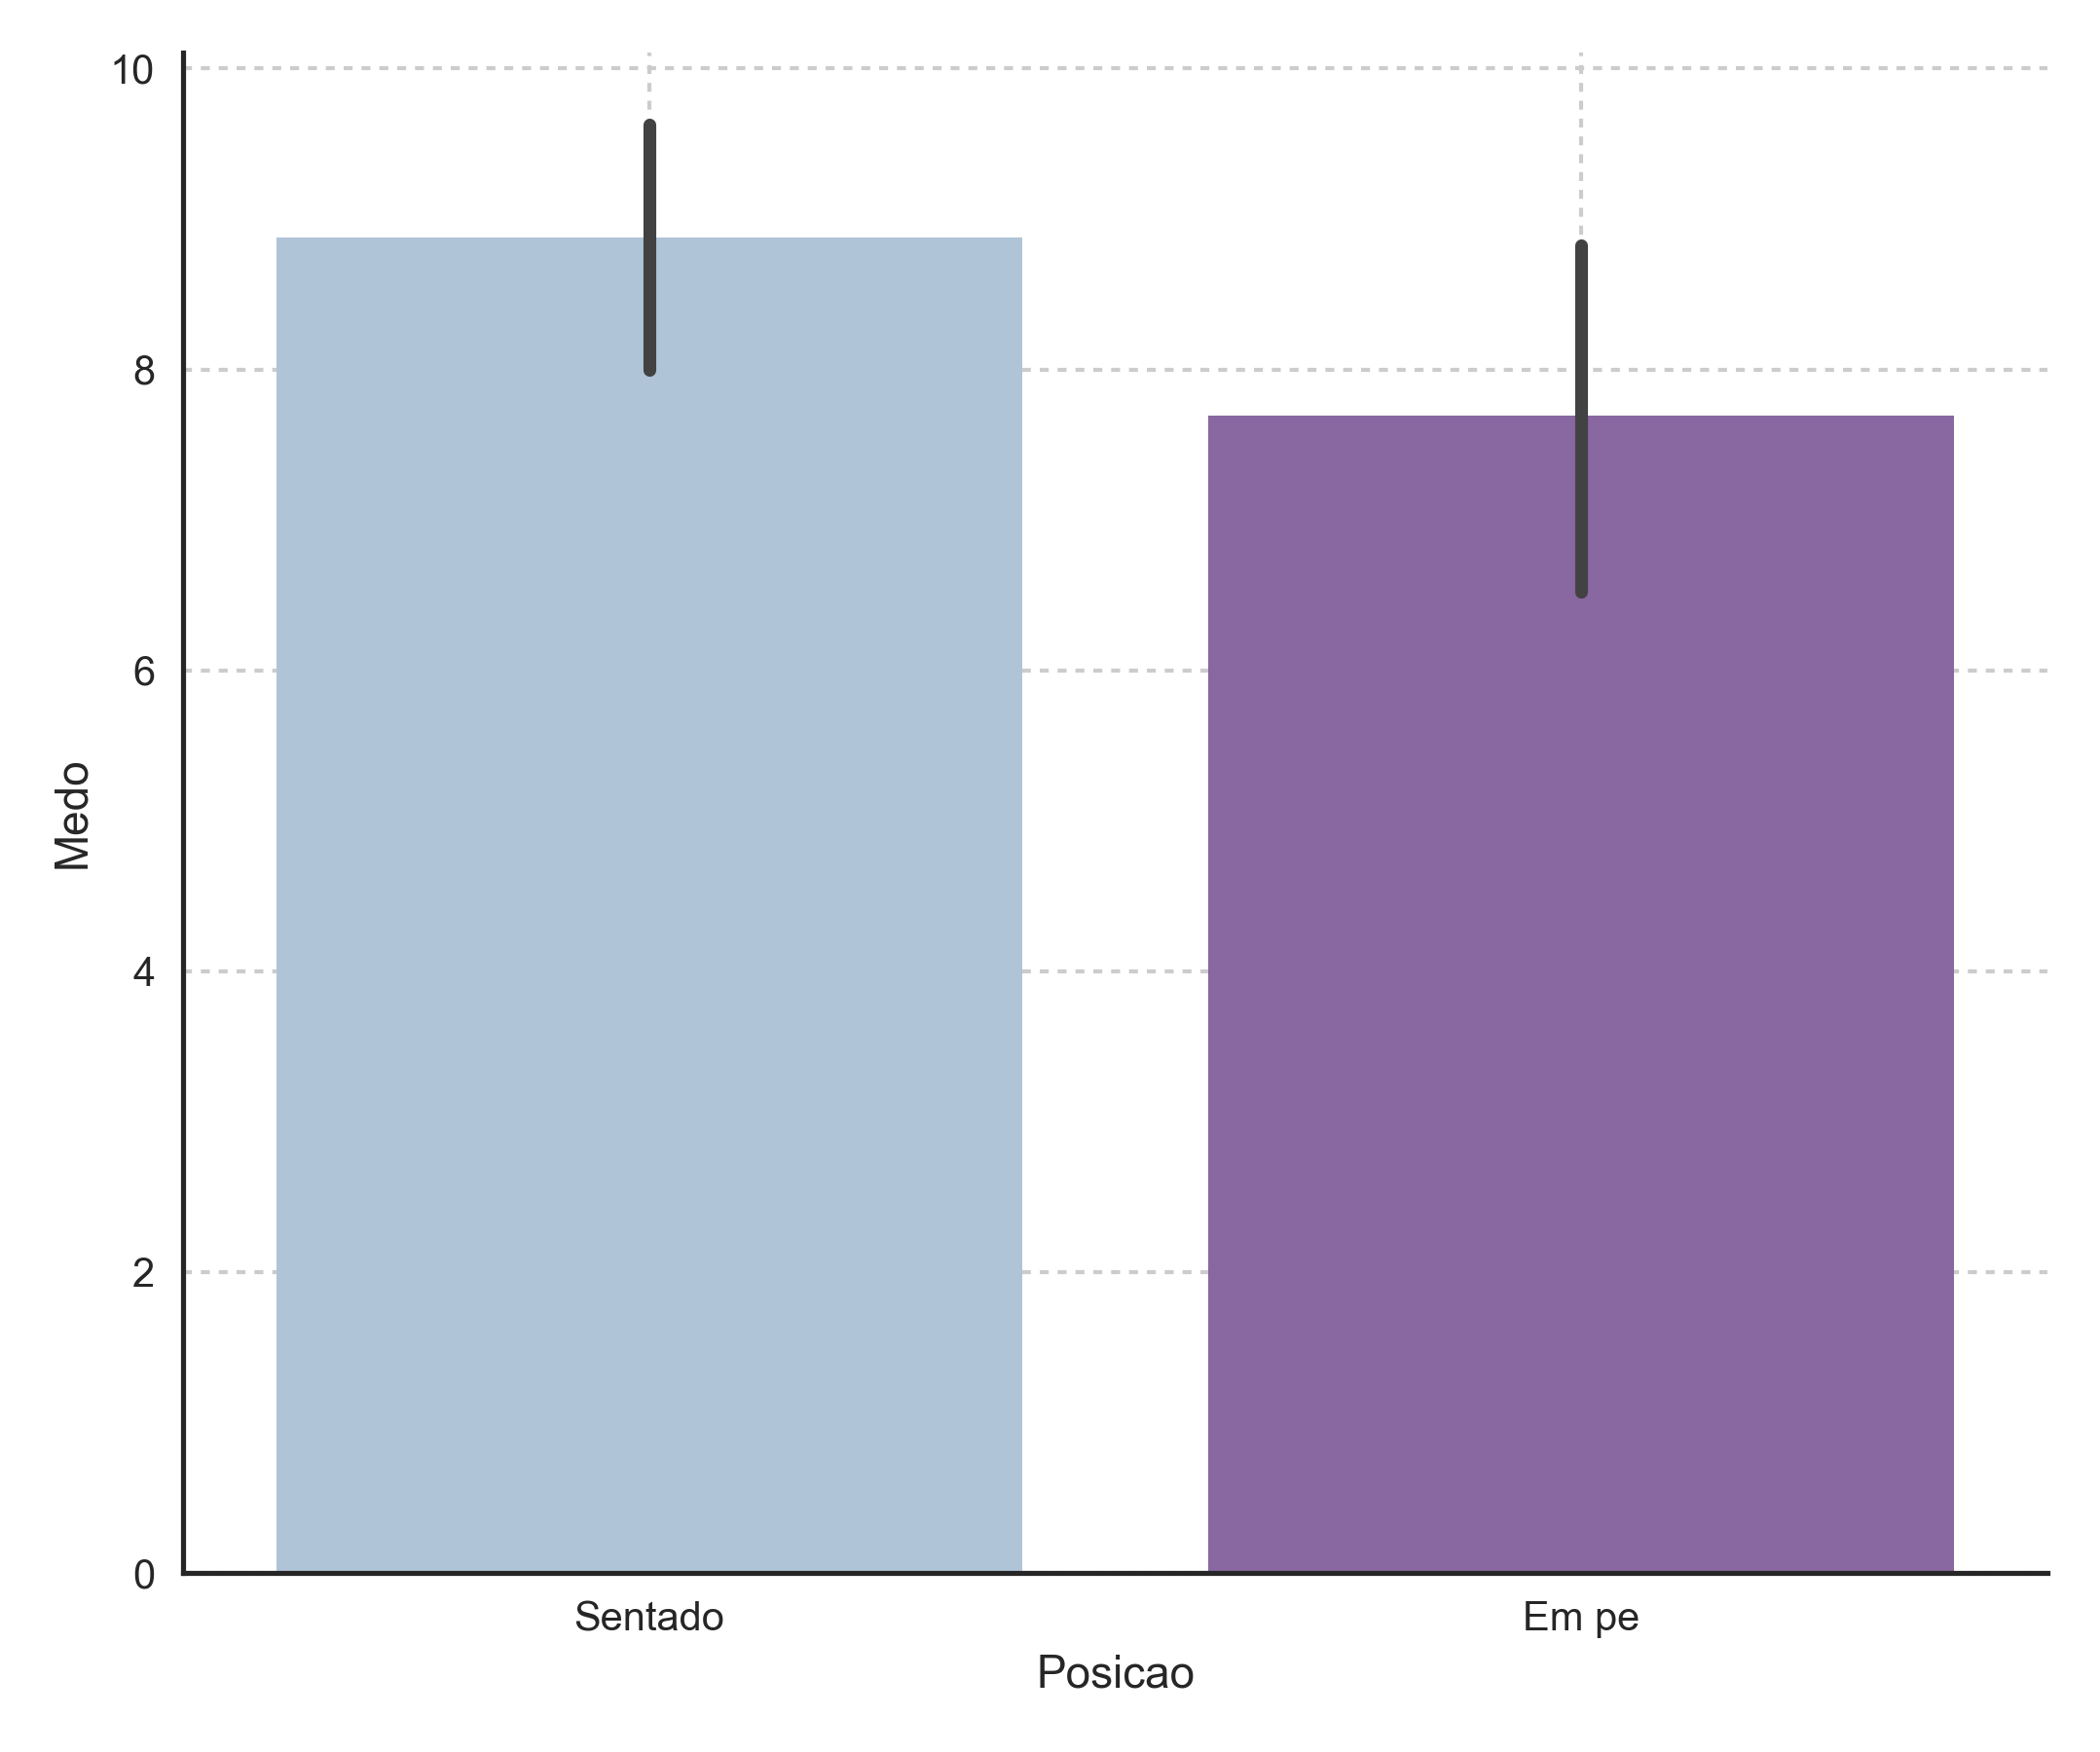
\includegraphics[width=\textwidth]{medo_posicao.png}
		\smallcaption{Fonte: O autor.}
		\label{fig:medoposicao}
	\end{minipage}
\end{figure}

Assim como em relação ao conforto do usuário, os participantes que sentiram mais medo do robô estavam em pé. Os participantes sentados apresentaram uma média de 8.8750, com desvio padrão de 1.6910. Comparando, os participantes em pé tiveram 7.6957 de média e um desvio padrão de 2.7731. O manipulador é um ponto de atenção na interação, principalmente quando está dentro do espaço social da pessoa. Os maiores índices de medo ocorreram por que o robô encostou o manipulador na pessoa, sem nenhum aviso prévio. As pessoas mais sociáveis sentiram menos medo que as menos sociáveis, como apresenta na figura~\ref{fig:medosociavel}. Na média as pessoas sociáveis apresentam 8.4688 contra 6.8571 das pessoas não sociáveis. Os desvios padrão apresentaram os valores 2.0461 e 3.5225, respectivamente.

\begin{figure}[ht!]
	\centering
	\begin{minipage}{0.65\textwidth}
		\caption{Medo por declaração de sociável.}
		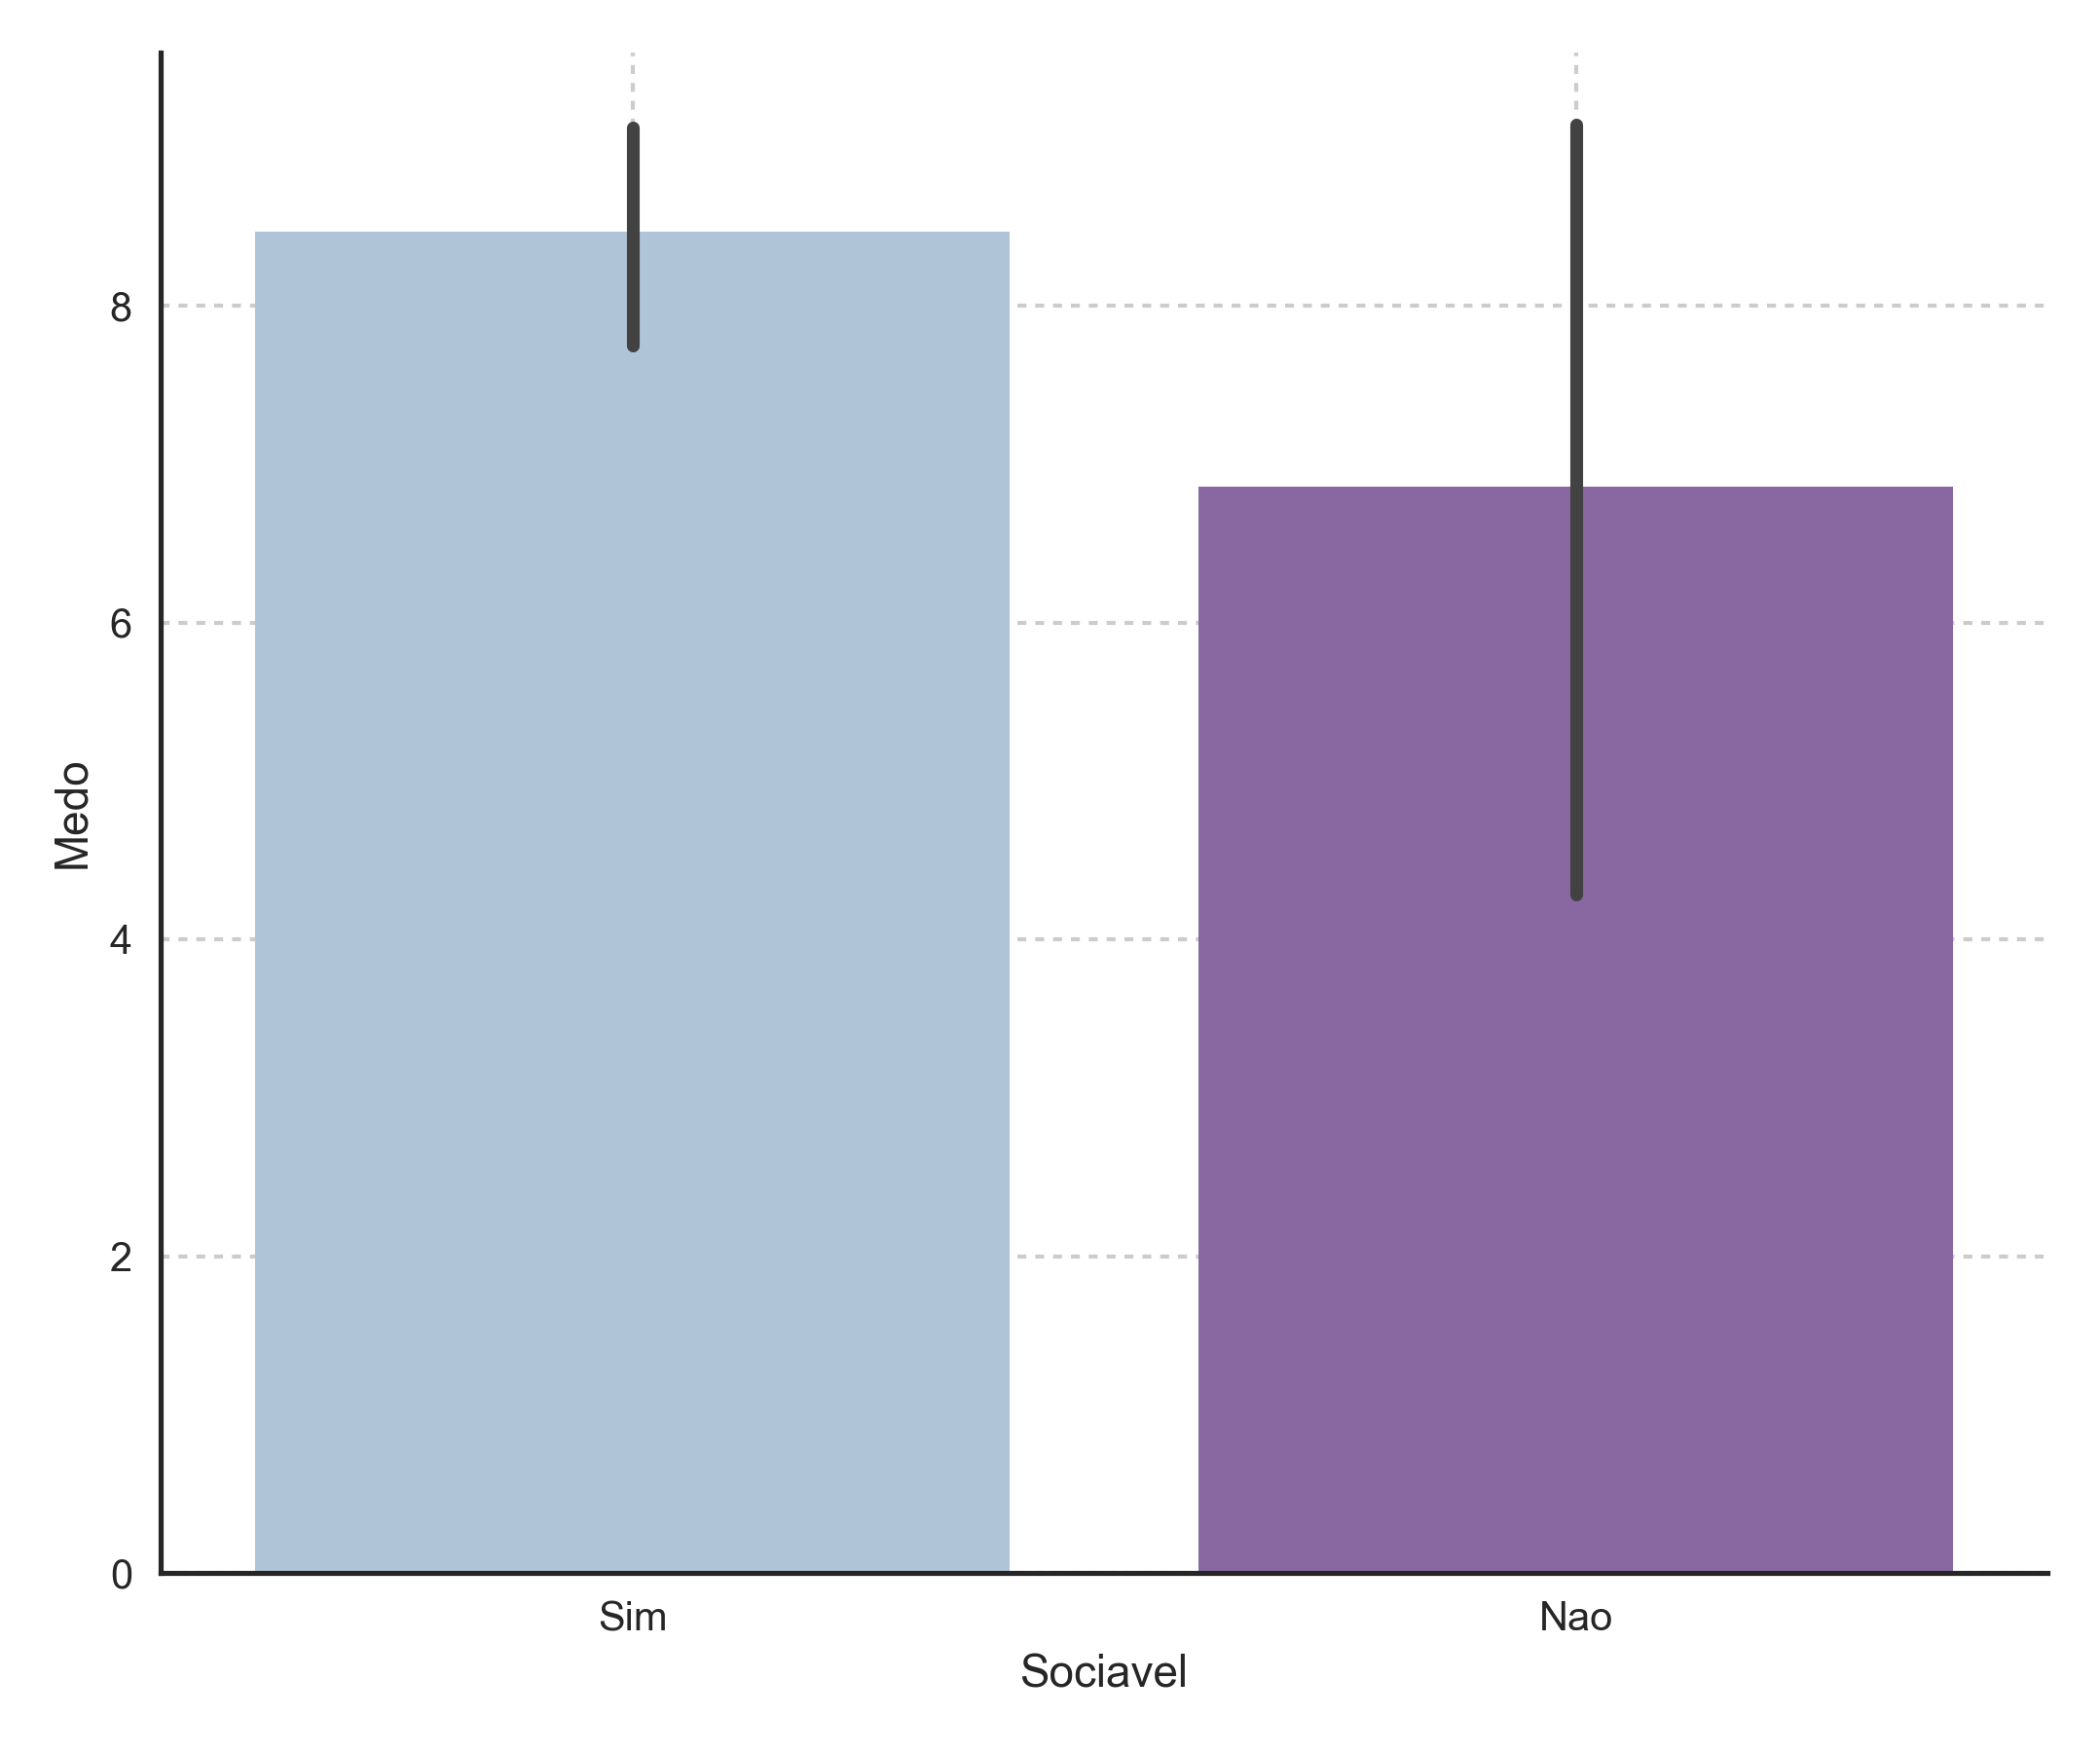
\includegraphics[width=\textwidth]{medo_sociavel.png}
		\smallcaption{Fonte: O autor.}
		\label{fig:medosociavel}
	\end{minipage}
\end{figure}

Após as análises gerais sobre as informações coletadas, é realizado o processo para obter os grupos de perfis de usuários, conforme seção~\ref{sec:criacaopersonas}. Para obter os grupos de perfis, utilizou-se o algoritmo de agrupamento por similaridade QG-SIM. Foram testados três valores Q, que determinam a similaridade mínima do grupo, para determinar os grupos. Os valores utilizados foram 0.6, 0.7 e 0.8. O valor 0.6 resultou em 3 grupos, porém um dos grupos manteve 90\% dos perfis e ou outros 10\% foram distribuídos entre os dois grupos restantes. O valor $Q = 0.6$ apresentou resultado muito generalizado e que não condiz com os perfis que realizaram os testes.

Quando aplicado o valor de 0.8 de similaridade para o algoritmo, 7 grupos foram encontrados. Nessa situação, os grupos ficaram bem específicos, sendo que 4 dos 7 grupos eram compostos por apenas 1 pessoa. Dessa maneira, é possível comprovar que o resultado gerado é muito especializado. Elevar o grau de similaridade nesse ponto, provavelmente serão encontrados mais grupos com apenas uma pessoa. Esse não é o objetivo da técnica de Personas. Então este resultado também foi desconsiderado.

O valor intermediário, 0.7, foi escolhido. Ele resultou em 5 grupos. Um grupo com 21 perfis, que resultou na Persona Joaquim (vide tabela~\ref{tab:joaquim}). Um grupo com 7 pessoas para Persona Maria Eduarda (vide tabela~\ref{tab:mariaeduarda}). Outro grupo com 9 pessoas deu origem a Persona Alfredo (vide tabela~\ref{tab:alfredo}). As outras duas Personas foram criadas com base em dois grupos de 1 pessoa. Apesar de serem formados por apenas 1 pessoa, algumas características foram totalmente descriminante. A Persona Manuel (vide tabela~\ref{tab:manuel}), por exemplo, não tem acesso, nem conta em redes sociais. E a Persona Danielo (vide tabela~\ref{tab:danielo}) aplicou a nota positiva máxima em todas as situações de interação. Esses fatores foram decisivos para que esses perfis permanecessem isolados em um grupo cada um.

Cada perfil dentro dos grupos mantém uma consistência etnográfica e também sobre a percepção em relação aos comportamentos e ações do robô. As percepções de cada perfil, estão sintetizadas e são apresentadas em grupos de informações similares. Essas informações auxiliaram na descrição de cada Persona. A tabela~\ref{tab:expectativacasa} apresenta um compilado das informações referentes a expectativa de ter um robô em casa, na percepção de cada usuário.

\begin{table}[!ht]
	\caption{Expectativa do robô em casa dos perfis por Persona.}
	\label{tab:expectativacasa}
	\centering
	\begin{tabular}{c | c | c }
        \hline
        \multicolumn{3}{c}{Expectativa do robô em casa?} \\ \hline
        Persona & Observação & Quantidade \\ \hline
        \multirow{7}{*}{Joaquim} & Limpar a casa & 7 \\
        \hhline{~--}
        & Buscar objetos & 1 \\
        \hhline{~--}
        & Cuidar da segurança & 1 \\
        \hhline{~--}
        & Obediência & 4 \\
        \hhline{~--}
        & Afetividade & 4 \\
        \hhline{~--}
        & Naturalidade & 3 \\
        \hhline{~--}
        & Respeito & 3 \\
        \hline
        \multirow{3}{*}{Maria Eduarda} & Realizar tarefas domésticas & 5 \\
        \hhline{~--}
        & Dirigir o carro & 1 \\
        \hhline{~--}
        & Amigável & 1 \\
        \hline
        \multirow{4}{*}{Alfredo} & Realizar tarefas domésticas & 5 \\
        \hhline{~--}
        & Comandos de voz & 2 \\
        \hhline{~--}
        & Obediência & 2 \\
        \hline
        Danielo & Realizar tarefas domésticas & 1 \\
        \hline
        Manuel & Atender necessidades & 1 \\
        \hline
    \end{tabular}
    \smallcaption{Fonte: O autor.}
\end{table}

A pergunta da expectativa do robô em casa foi realizada antes da interação com o robô. Com base nas respostas pode-se perceber que as pessoas, no geral, enxergam os robôs como ferramentas. Essa percepção muda após a interação e a demonstração das habilidades dos robôs. Em alguns casos, a mudança de opinião é nítida, onde comentários como ``ele faz tudo isso sozinho'' são mencionados durante o teste. Ou quando o usuário diz que imagina robôs apenas na linha de produção de fábricas e montadores. Outra questão discutida antes da interação com o robô é a expectativa sobre o papel dele, em relação ao ambiente de trabalho. As respostas compiladas são apresentadas na tabela~\ref{tab:expectativatrabalho}.

\begin{table}[!ht]
	\caption{Expectativa do robô no ambiente de trabalho dos perfis por Persona.}
	\label{tab:expectativatrabalho}
	\centering
	\begin{tabular}{c | c | c }
        \hline
        \multicolumn{3}{c}{Expectativa do robô no ambiente de trabalho?} \\
        \hline
        Persona & Observação & Quantidade \\
        \hline
        \multirow{10}{*}{Joaquim} & Obediência & 4 \\
        \hhline{~--}
        & Realizar tarefas & 7 \\
        \hhline{~--}
        & Indiferente sobre o robô no trabalho & 1 \\
        \hhline{~--}
        & Eficiência nas atividades & 2 \\
        \hhline{~--}
        & Comunicação & 1 \\
        \hhline{~--}
        & Antecipar tarefas & 1 \\
        \hhline{~--}
        & Gerenciador de \emph{TODO List} & 1 \\
        \hhline{~--}
        & Otimizar processos & 1 \\
        \hhline{~--}
        & Seja sociável & 1 \\
        \hhline{~--}
        & Agir com naturalidade & 2 \\
        \hline
        \multirow{3}{*}{Maria Eduarda} & Realizar tarefas & 4 \\
        \hhline{~--}
        & Eficácia & 1 \\
        \hhline{~--}
        & Amigável & 1 \\
        \hline
        \multirow{3}{*}{Alfredo} & Realizar tarefas & 6 \\
        \hhline{~--}
        & Rápido & 1 \\
        \hhline{~--}
        & Obediência & 1 \\
        \hline
        Danielo & Executar tarefas repetitivas & 1 \\
        \hline
        Manuel & Atender necessidades & 1 \\
        \hline
    \end{tabular}
    \smallcaption{Fonte: O autor.}
\end{table}

Apesar da expectativa no trabalho ser a realização de tarefas, em linhas gerais, alguns outros pontos foram levantados. Comunicação, naturalidade, ser amigável e sociável, além de outros adjetivos voltados para convívio social em ambientes corporativos. Essa percepção pode mostrar tendências para aceitar trabalho em equipe com robôs autonômos de maneira natural. As tabelas a seguir são de informações que foram coletadas após o experimento de interação social com o robô. A tabela~\ref{tab:agradou} apresenta as percepções sobre o robô, que os participantes mais e menos gostaram.

\begin{table}[!ht]
	\caption{O que os perfis mais gostaram e menos gostaram separados por Persona.}
	\label{tab:agradou}
	\centering
	\begin{tabular}{c | c | c | c | c}
        \hline
        \multirow{2}{*}{Persona} & \multicolumn{2}{c}{(+) Gostou} & \multicolumn{2}{c}{(-) Gostou} \\
        \hhline{~----}
		& Observação & Quantidade & Observação & Quantidade \\
		\hline
        \multirow{9}{*}{Joaquim} & Navegação & 4 & Desajeitado & 7 \\
        \hhline{~----}
		& Face & 12 & Tempo de localização & 2 \\
        & & & no ambiente &  \\
        \hhline{~----}
        & Voz & 6 & Barulho das rodas & 4 \\
        \hhline{~----}
        & Manipulador & 1 & Feedback baixo & 1 \\
        \hhline{~----}
        & & & Manipulador & 1 \\
        \hhline{~----}
		& & & Rodas & 1 \\
        \hhline{~----}
		& & & Fala autoritária & 1 \\
        \hhline{~----}
		& & & Tempo de resposta & 1 \\
        \hline
        \multirow{4}{*}{Maria Eduarda} & Navegação & 4 & Estrutura & 2 \\
        \hhline{~----}
        & Interação & 1 & Manipulador & 2 \\
        \hhline{~----}
        & Face & 3 & Barulho & 1 \\
		\hhline{~----}
        & & & Tempo de Resposta & 1 \\
        \hline
        \multirow{6}{*}{Alfredo} & Face & 2 & Tempo de Resposta & 2 \\
        \hhline{~----}
        & Voz & 2 & Desajeitada & 1 \\
        \hhline{~----}
        & Navegação & 1 & Manipulador & 3 \\
		\hhline{~----}
        & Feedback & 1 & Barulho & 1 \\
		\hhline{~----}
        & Toque & 1 & Perda da localização & 1 \\
		\hhline{~----}
        & Interação & 2 & & \\
        \hline
        Danielo & Interação & 1 & Barulho & 1 \\
        \hline
        Manuel & Face e voz & 1 & Manipulador & 1 \\
        \hline
    \end{tabular}
    \smallcaption{Fonte: O autor.}
\end{table}

Através da tabela~\ref{tab:agradou} é possível observar quais pontos do robô, e até como as variáveis de percepção do usuário que foram criadas com base nas heurísticas de interação (vide seção~\ref{sec:heuristicas}), se relacionam com cada perfil. A visibilidade do estado do robô é um dos pontos mais observados entre os usuários. A relação de \emph{feedback} do robô, algumas das Personas apontaram como positivo e outras como negativo, pois não foi realizado de maneira adequada. Outro ponto levantado, é a questão do barulho feito pela base do robô, onde 4 das 5 Personas observaram isso como um problema. Além dos pontos positivos e negativos do robô durante a interação, as informações sobre quais pontos geraram desconforto ou medo são importantes. As informações sobre desconforto são apresentadas na tabela~\ref{tab:desconforto}.

\begin{table}[!ht]
	\caption{Desconforto dos perfis na interação, separados por Persona.}
	\label{tab:desconforto}
	\centering
	\begin{tabular}{c | c | c }
        \hline
        Persona & Observação & Quantidade \\
        \hline
        \multirow{3}{*}{Joaquim} & Quase batida no ambiente & 1 \\
        \hhline{~--}
        & Primeira aproximação & 4 \\
        \hhline{~--}
        & Balanço da estrutura & 1 \\
        \hline
        \multirow{2}{*}{Maria Eduarda} & Manipulador & 1 \\
        \hhline{~--}
        & Aproximação & 1 \\
        \hline
        \multirow{3}{*}{Alfredo} & Falta de feedback & 2 \\
        \hhline{~--}
        & Toque & 1 \\
        \hhline{~--}
        & Aproximação & 2 \\
        \hline
        Danielo & -- & -- \\
        \hline
        Manuel & Manipulador & 1 \\
        \hline
    \end{tabular}
    \smallcaption{Fonte: O autor.}
\end{table}

Na tabela~\ref{tab:desconforto} pode-se evidenciar que a aproximação do robô, principalmente ao entrar no espaço pessoal e intímo da pessoa, gera um nível de desconforto significante. Quando ocorre o toque no participante esse desconforto pode levar a um nível de medo para alguns participantes na interação. O controle da aproximação e da invasão das zonas sociais definidas através da teoria de proximidade (capítulo~\ref{cap:proxemics}) é importante para melhorar a experiência do usuário e conseguir manter uma interação de longo prazo em outros cenários. As questões relacionadas a proximidade do robô, não condizem apenas com a ação de aproximição. A proximidade é um fator importante que pode influenciar em gestos, expressões faciais e até mesmo volume da voz emitida pelo robô.

Outro resultado apontado pelos questionários aplicados durante o experimento, tem relação com as questões culturais dos participantes. Uma das perguntas apresentadas no questionário de pré teste (vide tabela~\ref{tab:questoespreteste}), era a declaração de qual cultura o usuário mais se identifica. Um terço dos participantes declarou que se identifica com a cultura de um país diferente do seu de origem.

Esse indicativo apresentou um alerta para uma das hipóteses desta tese, onde é questionado que a cultura sobrepõe a experiência do usuário na interação social. Contudo, quando as Personas foram criadas, a cultura obtida através da medida de tendência central foi a do país de origem dos participantes. É possível assim, identificar que por mais que exista a declaração de uma cultura diferente por parte do usuário, a cultura de origem tem maior influência sobre suas ações. A experiência do usuário está ligada aos fatores culturais, podendo ter diferenças entre os costumes de cada cultura perante cada comportamento do usuário.

A partir dos testes iniciais para criação do classificador, novos teste devem ser executados para que haja a validação do classificador bayesiano de Personas. Na tabela~\ref{tab:perfilvalidacao} é apresentado informações sobre os 16 perfis dos usuários que realizaram o teste para validação do classificador bayesiano.

\begin{table}[!ht]
	\caption{Perfis dos 16 usuários que realizaram o teste de validação.}
	\label{tab:perfilvalidacao}
	\centering
	\begin{tabular}{c | c | c | c | c | c | c | c}
        \hline
        Idade & Altura & Gênero & Feição & Sociável? & Óculos & Cabelo & Etnia \\
         &  &  &  &  & de Grau? & Comprido? &  \\ \hline
		 25 & 1.86 & Masculino & Normal & Sim & Sim & Sim & Branca \\ \hline
		 34 & 1.82 & Masculino & Normal & Sim & Sim & Não & Branca \\ \hline
		 19 & 1.76 & Masculino & Normal & Sim & Não & Não & Branca \\ \hline
		 20 & 1.74 & Masculino & Séria/Fechada & Não & Sim & Não & Parda \\ \hline
		 21 & 1.70 & Masculino & Sorridente & Sim & Não & Não & Branca \\ \hline
		 26 & 1.68 & Masculino & Normal & Sim & Sim & Não & Parda \\ \hline
		 27 & 1.81 & Masculino & Séria/Fechada & Sim & Sim & Não & Branca \\ \hline
		 33 & 1.62 & Feminino & Normal & Sim & Sim & Sim & Branca \\ \hline
		 37 & 1.79 & Masculino & Normal & Sim & Sim & Não & Branca \\ \hline
		 37 & 1.79 & Masculino & Normal & Sim & Não & Não & Branca \\ \hline
		 20 & 1.56 & Masculino & Normal & Sim & Não & Não & Amarela \\ \hline
		 20 & 1.70 & Masculino & Normal & Não & Sim & Não & Branca \\ \hline
		 20 & 1.90 & Masculino & Normal & Não & Sim & Não & Parda \\ \hline
		 20 & 1.73 & Masculino & Normal & Sim & Sim & Não & Branca \\ \hline
		 29 & 1.59 & Feminino & Normal & Sim & Não & Sim & Branca \\ \hline
		 61 & 1.60 & Feminino & Sorridente & Sim & Sim & Sim & Branca \\ \hline
	\end{tabular}
	\smallcaption{Fonte: O autor.}
\end{table}

A tabela~\ref{tab:perfilvalidacao} apresenta as informações declaradas sobre todos os paritipantes do teste de para criação do classificador. Pode-se identificar os limites das variáveis dos parcipantes como, a idade mínima apresentada é de 19 anos e a máxima de 61 anos, com uma média de 28 anos e um desvio padrão de 11 anos. A relação entre altura das pessoas, a menor estatura foi de 1,59 m contra 1,90 m da maior. Na altura a média foi de 1,73 m, mantendo um desvio padrão de 0,11 m. No total foram 13 homens e 3 mulheres na amostra, distribuídos entre alunos da instituição de ensino e visitantes, todos com o mínimo de contato com robôs.

Durante os testes os participantes elogiaram o comportamento do robô durante toda a tarefa. As variáveis cognitivas criadas a partir das heurísticas de avaliação de usabilidade, foram questionados por grande parte dos participantes. As principais variáveis questionadas foram a visibilidade do estado do robô e a naturalidade dos gestos que o robô executou com o manipulador. Foram variáveis impactantes para determinar em qual Persona cada usuário se enquadra.

O ponto positivo dentre todos os comportamentos e ações do robô foram as expressões faciais. Alguns participantes ficaram com medo do robô quando se aproximou com uma expressão brava. Ao apresentar uma expressão triste, os participantes sentiam dó pelo robô não ter conseguido encontrar a sua garrafa. No geral, o comportamento dos participantes era como um novo membro da casa. Apenas um participante assossiou a um fato negativo a convivência do robô. Seu comentário foi ``Apesar de saber que foi devidamente programado, não me sentiria confortável em dividir o ambiente com um ser de polímero e metal com inteligência semelhante a minha''. Com base nesse comentário, pode-se dizer que o participante tem medo do robô começar a aprender a ser muito  mais que uma ferramenta e poder apresentar algum risco físico ao conviver em casa.

Pontos de atenção levantados pelos participantes sobre a presença do robô em casa é a preocupação com o design e o volume que o robô ocupará. São pontos importantes para o desenvolvimento do projeto e aceitação do robô dentro das casas. Outra questão que desagradou alguns dos participantes, foi o excesso de barulho na locomoção do robô pelo ambiente. A fala do robô também foi prejudicada pelo tipo de caixa de som que foi utilizado. O som saiu abafado e dificultou a compreensão do que o robô estava dizendo, principalmente quando o ambiente estava com um número maior de pessoas. A questão da caixa de som, identificou-se em um momento posterior aos testes, que o problema era falta de bateria nos alto faltantes. Elas tiveram que ser substituidas em alguns momentos do teste pelo som do próprio computador, responsável por executar todas as funções de controle do robô. Em questão sobre o papel do robô em uma residência, é unânime a opinião de que ele deva fazer as tarefas domésticas simples, porém que ocupam muito tempo das pessoas no dia-a-dia.

Para cada perfil selecionado a realizar o teste de validação, foi feito uma classificação manual com base nas respostas para comparação com o classificador bayesiano executado nos testes. Na classificação manual encontrou-se 7 perfis para a Persona Joaquim, 4 para a Maria Eduarda, 2 para Alfredo e Danielo, cada, e 1 para a Persona Manuel.

O trabalho de classificação automático foi realizado pelo \emph{software} SamIam, onde foi possível construir de maneira visual a rede bayesiana e determinar os valores das probabilidades condicionais, de acordo com o processo descrito na seção~\ref{sec:rede-bayesiana}. Na execução da rede bayesiana, eram atribuídos os valores dos nós de efeito, composto pelas variáveis de comportamentais de conforto, desconforto e medo. Também as variáveis de ações do robô e cenário de uso, como a posição do usuário na cena, além das variávies cognitivas criadas com base nas heurísticas de avaliação de usabilidade. Todo esse conjunto de variáveis fazem parte da camada de nós internos da rede bayesiana.

Os valores são atribuidos de acordo com cada situação executada durante o teste, e a evidência de conforto, desconforto e medo declarada pelo participante ou observada pelo especialista que acompanhava o teste. A partir dos valores atribuídos o classificador retorna os valores dos nós pais, no caso as Personas, dizendo qual a probabilidade de ser cada Persona. A maior probabilidade define a Persona que o classificador escolheu. Durante a classificação a rede bayesiana conseguiu uma taxa de 68,75\% de acerto.

As Personas Joaquim e Alfredo, foram as que mais existiram trocas durante a classificação. O motivo dessa troca de perfis na classificação ocorreu, pois os dois perfis são bem parecidos. Ambas Personas possuem o comportamento muito similar, são pequenos detalhes sobre o conforto que fizeram a classificação sair diferente da esperada.

Um outro fator que gerou essa diferença entre os classificadores manual e bayesiano foram as bases de classificação. O manual tem como base os questionários pré interação, que são as informações que foram mais relevantes ao algoritmo de agrupamento para composição das Personas. Já o classificador bayesiano tem como base a interação entre o robô e o ser humano. Dessa maneira, podem ocorrer situações de comportamentos da pessoa que não foram mapeadas e impactem no resultado final da classificação. Por exemplo, durante o questionário e entrevista pré teste, o participante informa que está confortável com o teste e não tem problema nenhum ao interagir com o robô. E quando inicia o teste de interação o robô apresenta um comportamento que gera uma experiência ao participante diferente da mapeada anteriormente. Essa situação faz com que a classificação do perfil seja feita diferente da manual.

Essa classificação pode ser correta em um contexto de uso diferente, ou até mesmo de acordo com o estado emocional do participante. Porém, essas variações não foram abordadas nos experimentos realizados nessa tese. A taxa de acerto na classificação de cada Persona ficou da seguinte maneira, Joaquim foi classificado com 71\% de acerto, Maria Eduarda 75\%, Alfredo com 50\%, Danielo 100\% e Manuel foi a Persona com menos acertos, a taxa foi de 0\%. Porém, a Persona Manuel só teve um perfil que se enquadrasse como ela. Essa taxa pode ser melhorada, com a execução de novos testes para ajustar os valores das probabilidades condicionais. Um outro método para que seja feito uma melhor distribuição dos valores de probabilidades entre os nós é o uso de um algortimo de aprendizagem.

O uso de uma especificação de projeto para interação humano-robô seguindo os passos apresentados na seção~\ref{sec:projetoihr} foram essenciais em diversos pontos do projeto. O uso das Personas no classificador bayesiano só foi possível dado a especificação do contexto de uso. Sem a definição do contexto de uso, não seria plausível utilizar a técnica de Personas. Esse classificador pode ter uma variação das tabelas de probabilidades condicionais, em contextos de uso diferentes. Assim, como novas variáveis podem ser essenciais na estrutura da rede bayesiana. Um estudo mais aprofundado sobre o comportamento do classificador em outros contextos de uso deve ser realizado. Assim, a proposta pode evoluir para diferentes contextos de uso e novos cenários de atuação. Uma possível solução para utilizar o classificador em outros contextos de uso, é criar uma tabela de probabilidade condicional da rede bayesiana para cada contexto novo. Assim, o robô percebendo qual o contexto que ele se encontra, pode automaticamente ajustar os valores da tabela de probabilidade condicional.

Além do contexto de uso, outro ponto fundamental que o projeto auxiliou, foi quando a base do robô utilizada nos testes pilotos quebrou. A troca por uma nova base poderia ter sido traumática ao projeto. Porém, com a arquitetura bem definida e o software desenvolvido utilizando padrões de projeto que preveem a adaptação de outros componentes com a mesma função, foi praticamente uma troca \emph{plug'n play} realizada entre as bases. Pequenos ajustes foram necessários, como a posição dos sensores utilizados na base como o \emph{laser}. A criação do projeto também possibilitou que novos componentes possam ser inseridos na proposta feita por essa tese. Por exemplo, os componentes para adaptação do comportamento do robô após a classificação do usuário. Outros componentes que podem ser inseridos são os de identificação de medo, conforto e desconforto de maneira automática. Sem a especificação do projeto de maneira sistêmica a expansão através desses componentes não seria possível.

Quando é analisado o projeto em relação aos 5 (cinco) fatores que impactam a experiência do usuário, apresentado no capítulo~\ref{cap:ux}, percebe-se que o projeto gerou uma experiência satisfatória aos participantes. Porém, existem diversos aspectos que devem evoluir ao longo de seu contínuo desenvolvimento. O primeiro fator é a utilidade do produto para o usuário. Nos comentários feitos sobre a expectativa do conviver com o robô em casa e no trabalho, é possível notar que a utilidade para o robô móvel é alta e esperada por todos os participantes do teste. Outro fator de qualidade da experiência do usuário é a integridade funcional. Nesse fator o projeto precisa de alguns cuidados, pois existiram em alguns testes a falha de leitura de sensores como \emph{laser} e odometria, que levaram a falha do sistema. Os casos de falha, foram em muitos casos, incapazes de se auto recuperar. A falta de integridade pode trazer uma aparência de produto inacabado, gerando problemas de adesão ao robô no ambiente social.

Em questão de usabilidade, o robô necessita de melhorar alguns aspectos para proporcionar uma fácil interação. Como grande parte de sua comunicação é realizada através de voz, possibilitar outros idiomas além do inglês tornaria o uso melhor para alguns dos participantes do teste. Além disso, um projeto de manipulador que faça movimentos mais próximos do natural ao ser humano. A falta de naturalidade em relação aos gestos realizados pelo manipulador, gerou a falta do fator de persuasividade. Em vários momentos, ao qual o gesto foi utilizado para comunicar algo ao usuário, não foi possível compreender exatamente o que o robô gostaria de fazer. Esse é um ponto que precisa de evolução nos próximos ciclo de iteração para evolução no projeto. A aparência, último fator apresentado por~\textcite{hartson:2012}, apresentou pontos positivos e outros negativos, em uma menor proporção. O \emph{tablet} com as faces ajudaram a extrair boas reações dos participantes durante a interação. Inclusive as faces com expressões de tristeza e raiva, também causaram reações positivas dos participantes. Em relação a aparência, o ponto negativo do projeto foi o corpo do robô. Alguns participantes disseram que ele parecia estar inacabado, pois a carenagem do robô aparentava que iria desmontar em alguns movimentos. No geral, os cinco fatores de impacto à experiência de usuário, foram atendidos de maneira positiva entre os participantes do teste.



% %!TEX root=Principal.tex
\chapter{CONCLUSÕES PARCIAIS}
\label{cap:conclusoes}
De acordo com os estudos realizados na literatura existente, é possível perceber que a criação de um \emph{framework} para interação humano-robô capaz de aprender e se adaptar ao comportamento de uma pessoa torna-se viável e essencial a partir do momento que a popularização da robótica está cada vez maior, principalmente em ambientes domésticos para fins de ajuda ao ser humano.

Para a interação ocorrer de maneira efetiva é necessário que o robô saiba respeitar os limites espaciais do ser humano e também ao realizar uma aproximação ou movimento em direção a pessoa, estes devem ser delicado o suficiente para que não gere nenhum desconforto ou medo. Por exemplo, durante uma apresentação do robô PeopleBot para alunos e professores do ensino médio, percebeu-se que a aproximação do robô pode causar um certo desconforto e medo dependendo, em especial quando a pessoa não estava esperando essa aproximação e não era avisada sobre a ação. 

Quando o robô se locomovia em direção a pessoa sem nenhum anúncio prévio, essa pessoa por muitas vezes ficava com medo. O medo em algumas situações observadas era tão evidente que a pessoa deixa o mesmo ambiente que o robô estava. Porém, quando o robô se aproximava e era anunciado pelo apresentador, as pessoas ficavam paradas deixando o robô chegar a alguns poucos centímetros dela. 

As observações a partir desse experimento reforçam a importância de ter um componente de interação adaptativo para que o robô possa identificar o perfil comportamental e personalidade do indivíduo de tal forma que eles possam conviver no mesmo ambiente em uma maneira confortável e sem medo por parte do ser humano.

Esse componente deve ainda ser capaz de transferir o conhecimento adquirido a partir de um robô para outros robôs, levando em consideração não só as características da pessoa, mas também as características do robô, pois esses fatores podem influenciar no comportamento das pessoas e robôs durante a interação. As características do robô são muito importantes para determinar a forma de interagir, já que existem robôs em diversos formatos como quadrutores, direção diferencial, bípede, quadrupede, com ou sem manipuladores, com tamanhos diferentes e também o nível de ruído de cada robô. Todas essas variáveis devem ser consideradas em estudos futuros, mas já devem estar contempladas pelo \emph{framework} que é um dos produtos finais dessa tese.
% %!TEX root=Principal.tex
\chapter{CRONOGRAMA}
\label{cap:cronograma}
Nesse capitulo é apresentado o cronograma definido para a conclusão da tese. O início do cronograma é demarcado a partir da apresentação do exame de qualificação, conforme apresentado na figura~\ref{fig:cronograma}.

\begin{figure}[ht!]
	\centering
	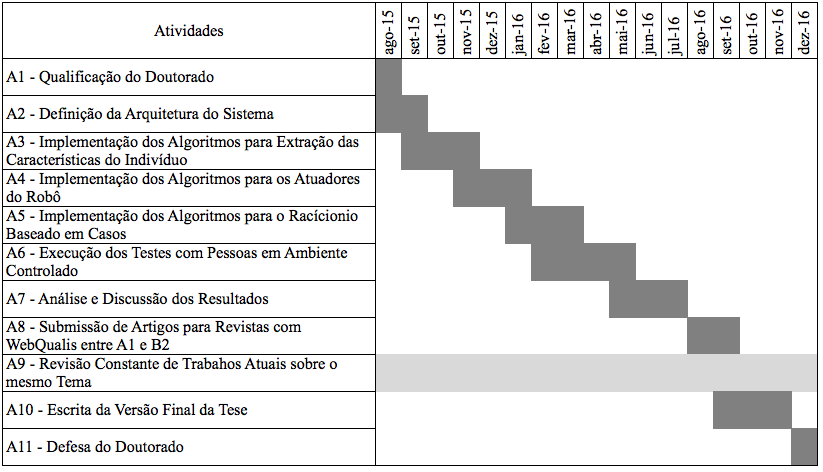
\includegraphics[width=\textwidth]{cronograma.png}
	\caption{Cronograma para Conclusão da Tese.}
	\label{fig:cronograma}
\end{figure}

A lista a seguir apresenta com mais detalhes as tarefas apresentadas no cronograma da figura~\ref{fig:cronograma}.

\begin{enumerate}
	\item \textbf{A1}: Apresentação do Exame de Qualificação para o Doutorado;
	\item \textbf{A2}: Definição da Arquitetura que irá auxiliar o desenvolvimento e execução do Sistema que poderá ser consumido por diferentes tipos de robô ao mesmo tempo;
	\item \textbf{A3}: Desenvolvimento dos algoritmos que serão utilizados para fazer com que o robô possa extrair as informações comportamentais das pessoas, de acordo com o apresentado na seção~\ref{sec:extracaocaracteristicas};
	\item \textbf{A4}: Desenvolvimento dos algoritmos que irão controlar os atuadores do robô, como por exemplo, cabeça, manipulador e motores;
	\item \textbf{A5}: Desenvolvimento dos algoritmos que compõem o mecanismo para Raciocínio Baseado em Casos, responsável pelo aprendizado de interação do robô;
	\item \textbf{A6}: Execução dos testes de interação de acordo com o descrito no capitulo~\ref{cap:testes};
	\item \textbf{A7}: Análise dos resultados utilizando métodos estatísticos e também as observações obtidas durante o acompanhamento dos testes de interação;
	\item \textbf{A8}: Submissão de pelo menos 2 artigos sobre a tese para revistas relevantes para a área de pesquisa, classificadas de acordo com o WebQualis da CAPES entre os níveis de A1 à B2;
	\item \textbf{A9}: Revisão bibliográfica contínua para certificar da originalidade e atualidade do trabalho de tal forma, que sua contribuição possa ajudar o avanço da área de pesquisa em robótica social e assistiva;
	\item \textbf{A10}: Consolidação do trabalho no texto do documento da tese para entrega à banca avaliadora;
	\item \textbf{A11}: Apresentação da Defesa para o título de Doutor.
\end{enumerate}


\bibliography{biblio}
\end{document}